%-------------------------------------------------------------------------------
%                      Template Naskah Skripsi
%               	Berdasarkan format JTETI FT UGM
% 						(c) @gunturdputra 2014
%-------------------------------------------------------------------------------

%Template pembuatan naskah skripsi.
\documentclass{jtetiskripsi}

\renewcommand \thesection{\Alph{section}.}
\renewcommand \thesubsection{\arabic{subsection}.}

%Untuk prefiks pada daftar gambar dan tabel
\usepackage[titles]{tocloft}
\renewcommand\cftfigpresnum{Gambar\	}
\renewcommand\cfttabpresnum{Tabel\	}

%Untuk hyperlink dan table of content
\usepackage[hidelinks]{hyperref}
\newlength{\mylenf}
\settowidth{\mylenf}{\cftfigpresnum}
\setlength{\cftfignumwidth}{\dimexpr\mylenf+2em}
\setlength{\cfttabnumwidth}{\dimexpr\mylenf+2em}

%comment
%\usepackage{comment}

%Untuk Bold Face pada Keterangan Gambar
\usepackage[labelfont=bf]{caption}

%Untuk caption dan subcaption
\usepackage{caption}
\usepackage{subcaption}

%pdf
\usepackage{pdfpages}

%table
\usepackage{graphics}

\usepackage{wrapfig}

%bibliography
\usepackage{natbib}

%equation
\usepackage{amsmath}

%algoritma
\usepackage{algorithm}
\usepackage{algpseudocode}

%listing
\usepackage{listings}
\usepackage{longtable}
\usepackage{multirow}

\lstset{
    language=Python,
    backgroundcolor=\color{white},   
    commentstyle=\color{black},
    keywordstyle=\color{black},
    numberstyle=\tiny\color{black},
    stringstyle=\color{black},
    basicstyle=\ttfamily\scriptsize,
    breakatwhitespace=false,         
    breaklines=true,                 
    captionpos=b,                    
    keepspaces=true,                 
    numbers=left,                    
    numbersep=7pt,                  
    showspaces=false,                
    showstringspaces=false,
    showtabs=false,                  
    tabsize=2,
    frame=single
}

%-----------------------------------------------------------------
%Disini awal masukan untuk data proposal skripsi
%-----------------------------------------------------------------
\titleind{Aplikasi Pengkajian Luka Berbasis Android Terintegrasi Dengan Sistem Informasi Klinik Keperawatan Luka}

\fullname{Muhammad Ardani}

\idnum{1313618014}

%\approvaldate{12 Februari 2019}
%\approvaldate{12 Februari 2019}

\degree{Sarjana Ilmu Komputer}

\yearsubmit{2025}

\program{Ilmu Komputer}

\dept{Ilmu Komputer}

\firstsupervisor{Muhammad Eka Suryana, M. Kom.}
\firstnip{198512232012121002}

\secondsupervisor{Drs. Mulyono, M.Kom.}
\secondnip{196605171994031003}

%-----------------------------------------------------------------
%Disini akhir masukan untuk data proposal skripsi
%-----------------------------------------------------------------

\tolerance=1
\emergencystretch=\maxdimen
\hyphenpenalty=10000
\hbadness=10000

\begin{document}

\cover
%-----------------------------------------------------------------

%-----------------------------------------------------------------
%Disini akhir masukan untuk muka skripsi
%-----------------------------------------------------------------
\chapter*{\centering{\large{LEMBAR PENGESAHAN}}}

\begin{figure}[H]
	\centering
	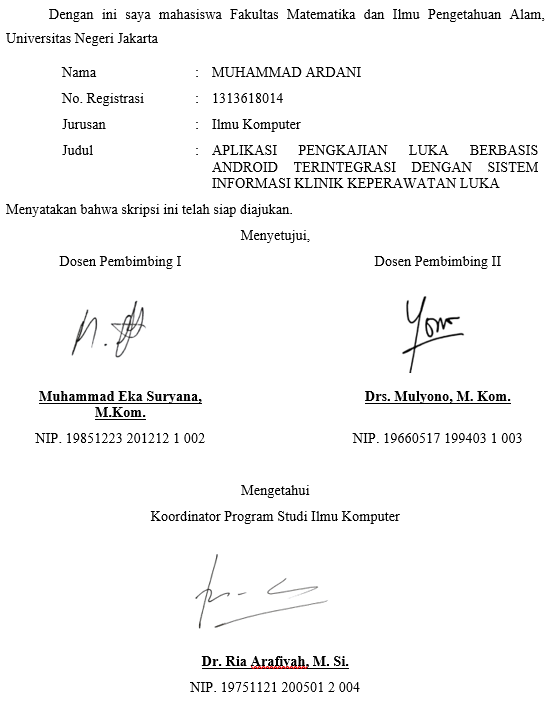
\includegraphics[keepaspectratio,width=0.95\textwidth, height=0.95\textheight]{gambar/lembar-pengesahan}
\end{figure}
\addcontentsline{toc}{chapter}{LEMBAR PENGESAHAN}
\chapter*{\centering{\large{LEMBAR PERNYATAAN}}}

Saya menyatakan dengan sesungguhnya bahwa skripsi dengan judul “Aplikasi Pengkajian Luka Berbasis Android Terintegrasi Dengan Sistem Informasi Klinik Keperawatan Luka” yang disusun sebagai syarat untuk memperoleh gelar Sarjana Komputer dari Program Studi Ilmu Komputer Universitas Negeri Jakarta adalah karya ilmiah saya dengan arahan dari dosen pembimbing.
Sumber informasi yang diperoleh dari penulis lain yang telah dipublikasikan dan disebutkan dalam teks skripsi ini, telah dicantumkan dalam Daftar Pustaka sesuai dengan norma, kaidah dan etika penulisan ilmiah.
Jika dikemudian hari ditemukan sebagian besar skripsi ini bukan hasil karya saya sendiri dalam bagian bagian tertentu, saya bersedia menerima sanksi pencabutan gelar akademik yang saya sanding dan sanksi-sanksi lainnya sesuai dengan peraturan perundang-undangan yang berlaku.


\vspace{4cm}

\begin{tabular}{p{8,4cm}r}
	&Jakarta, 07 Februari 2025\\
	&\\
	&\\
	&\\
	&Muhammad Ardani\\
	&1313618014              
\end{tabular}
\addcontentsline{toc}{chapter}{LEMBAR PERNYATAAN}
\chapter*{\centering{\large{HALAMAN PERSEMBAHAN}}}
\null\vfill
\begin{flushright}
\textit{Untuk Keluargaku dan Diriku Sendiri.}
\end{flushright}
\addcontentsline{toc}{chapter}{HALAMAN PERSEMBAHAN}
\chapter*{\centering{\large{ABSTRAK}}}

\begin{spacing}{1}
\textbf{MUHAMMAD ARDANI}. Aplikasi Pengkajian Luka Berbasis Android Terintegrasi Dengan Sistem Informasi Klinik Keperawatan Luka. Skripsi. Program Studi Ilmu Komputer Fakultas Matematika dan Ilmu Pengetahuan Alam, Universitas Negeri Jakarta. 2025. Di bawah bimbingan Muhammad Eka Suryana, M.Kom dan Drs. Mulyono, M.Kom.
\newline
\newline
Penyebab luka kronis dan faktor yang mempengaruhi penyembuhan luka cukup kompleks dan beragam. Dalam proses diagnosis, pengobatan dan manajemen luka kronis, dokter dan perawat perlu memiliki pemahaman menyeluruh serta kelengkapan rekam medis, manajemen yang efektif dan pemantauan kondisi fisik umum pasien secara tepat waktu, laporan pemeriksaan laboratorium, penilaian dan pengobatan luka fraksional. Secara umum, proses pengkajian luka masih dilakukan secara tradisional dengan metode pencatatan atau pengarsipan berbasis kertas. Saat ini, data-data tersebut masih dicatat secara manual, yang berisiko menimbulkan kesalahan dalam perhitungan. Selain itu, penelitian sebelumnya memiliki kekurangan penilaian data pengkajian luka kronis secara akurat. Sehingga diperlukannya penelitian ini dengan tujuan untuk membuat aplikasi pengkajian luka kronis dengan modul \textit{Bates-Jensen Assessment Wound Tools}(BWAT) berbasis \textit{Android}. Data kajian yang digunakan dalam penelitian ini terfokus pada proses pencatatan pasien berobat penanganan luka kronis. Proses pengembangan sistem ini menggunakan metode \textit{Scrum} dan seluruh aplikasi yang dibuat menggunakan bahasa pemrograman \textit{Kotlin} dan diintegrasi dengan penelitian-penelitian sebelumnya. Hasil akhir dari penelitian ini berupa aplikasi pengkajian luka yang membantu perawat dalam melakukan pencatatan proses penyembuhan luka pasien dan pasien dapat melihat progres penyembuhan dirinya sendiri.
\newline
\newline
\noindent \textbf{Kata kunci}: \textit{android, aplikasi, luka kronis, BWAT, scrum, pencatatan, integrasi}
\end{spacing}
\addcontentsline{toc}{chapter}{ABSTRAK}
\chapter*{\centering{\large{ABSTRACT}}}

\begin{spacing}{1}
\textbf{MUHAMMAD ARDANI}. Android-Based Wound Assessment Application Integrated with the Wound Care Clinic Information System. Thesis. Computer Science Study Program, Faculty of Mathematics and Natural Sciences, Universitas Negeri Jakarta. 2025. Supervised by Muhammad Eka Suryana, M.Kom, and Drs. Mulyono, M.Kom.
\newline
\newline
\textit{The causes of chronic wounds and the factors influencing wound healing are quite complex and diverse. In the process of diagnosing, treating, and managing chronic wounds, doctors and nurses need to have a comprehensive understanding, complete medical records, effective management, and timely monitoring of the patient's general physical condition, laboratory examination reports, wound assessment, and fractional wound treatment. In general, wound assessment is still carried out traditionally using paper-based recording or archiving methods. Currently, this data is still recorded manually, which poses a risk of calculation errors. Moreover, previous research lacked an accurate assessment of chronic wound evaluation data. Therefore, this study aims to develop a chronic wound assessment application with the Bates-Jensen Assessment Wound Tools (BWAT) module based on Android. The assessment data used in this study focuses on recording patients undergoing chronic wound treatment. The system development process follows the Scrum methodology, and the entire application is built using the Kotlin programming language while integrating findings from previous research. The final result of this study is a wound assessment application that assists nurses in documenting the wound healing process and enables patients to track their own healing progress.}
\newline
\newline
\noindent \textbf{\textit{Key}}: \textit{android, application, chronic wounds, BWAT, Scrum, documentation, integration}
\end{spacing}
\addcontentsline{toc}{chapter}{ABSTRACT}
\chapter*{\centering{\large{KATA PENGANTAR}}}

Puji syukur penulis panjatkan ke hadirat Allah SWT, karena dengan rahmat dan karunia-Nya, penulis dapat menyelesaikan skripsi yang berjudul \textbf{"Aplikasi Pengkajian Luka Berbasis Android Terintegrasi Dengan Sistem Informasi Klinik Keperawatan Luka"}.

Keberhasilan dalam menyusun skripsi ini tidak lepas dari bantuan berbagai pihak yang mana dengan tulus dan ikhlas memberikan masukan guna sempurnanya skripsi ini. Oleh karena itu dalam kesempatan ini, dengan kerendahan hati penulis mengucapkan banyak terima kasih kepada:

\begin{enumerate}

	\item{Yth. Para petinggi di lingkungan FMIPA Universitas Negeri Jakarta.}
	\item{Yth. Ibu Dr. Ria Arafiyah, M. Si selaku Koordinator Program Studi Ilmu Komputer.}
	\item{Yth. Bapak Muhammad Eka Suryana, M.Kom selaku Dosen Pembimbing I yang telah membimbing, mengarahkan, serta memberikan saran dan koreksi terhadap skripsi ini.}
	\item{Yth. Bapak Drs. Mulyono, M.Kom selaku Dosen Pembimbing II yang telah membimbing, mengarahkan, serta memberikan saran dan koreksi terhadap skripsi ini.}
	\item{Ibu Ns. Ratna Aryani, M.Kep yang senantiasa berpartisipasi dalam pembuatan aplikasi dalam skripsi saya.}
	\item{Orang tua penulis yang selama ini telah mendukung dan membantu menyelesaikan pengerjaan skripsi ini.}
	\item{Teman-teman Program Studi Ilmu Komputer 2018 yang telah mendukung dan membantu pengerjaan skripsi ini.}
	\item{Teman-teman dari Skripsi Victory yang turut mendukung penulis dalam pengerjaan skripsi ini.}
	\item{Teman-teman dari grup mabar Valorant yang senantiasa hadir untuk mendukung penulis dalam proses pengerjaan skripsi ini.}
	\item{Teman-teman dari grup Anti Scanning yang selalu menemani penulis dalam pengerjaan skripsi ini.}
	
	
\end{enumerate}

Penulis menyadari bahwa penyusunan skripsi ini masih jauh dari sempurna karena keterbatasan ilmu dan pengalaman yang dimiliki. Oleh karenanya, kritik dan saran yang bersifat membangun akan penulis terima dengan senang hati. Akhir kata, penulis berharap tugas akhir ini bermanfaat bagi semua pihak khususnya penulis sendiri. Semoga Allah SWT senantiasa membalas kebaikan semua pihak yang telah membantu penulis dalam menyelesaikan skripsi ini.

\vspace{4cm}

\begin{tabular}{p{7.5cm}c}
	&Jakarta, 13 Juni 2023\\
	&\\
	&\\
	&\\
	&Muhammad Ardani
\end{tabular}
\addcontentsline{toc}{chapter}{KATA PENGANTAR}
\tableofcontents 
\addcontentsline{toc}{chapter}{DAFTAR ISI}
\listoffigures
\addcontentsline{toc}{chapter}{DAFTAR GAMBAR}
\listoftables
\addcontentsline{toc}{chapter}{DAFTAR TABEL}

\begin{counterpage}
\end{counterpage}
%Disini awal masukan untuk Bab
%-----------------------------------------------------------------
%!TEX root = ./template-skripsi.tex
%-------------------------------------------------------------------------------
% 								BAB I
% 							LATAR BELAKANG
%-------------------------------------------------------------------------------

\chapter{PENDAHULUAN}

\section{Latar Belakang Masalah}

Lebih dari 13 juta orang di seluruh dunia menderita luka kronis setiap tahun. Jika luka kronis tidak sembuh dalam waktu lama, maka akan memperburuk kualitas hidup pasien dan keluarganya, yang mengakibatkan penyebaran infeksi atau bahkan komplikasi yang mengancam jiwa. Diagnosis, pengobatan, dan manajemen luka kronis yang efektif sangat penting dalam praktik klinis. Namun, penyebab luka kronis dan faktor yang mempengaruhi penyembuhan luka cukup kompleks dan beragam. Dalam proses diagnosis, pengobatan dan manajemen luka kronis, dokter dan perawat perlu memiliki pemahaman menyeluruh serta kelengkapan rekam medis, manajemen yang efektif dan pemantauan kondisi fisik umum pasien secara tepat waktu, laporan pemeriksaan laboratorium, penilaian dan pengobatan luka fraksional. \citep{wang2018new}. Berikut data luka kronis diabetes mellitus secara global berdasarkan DALYs.

\begin{table}[H]
	\caption{Diabetes Mellitus DALYs (\textit{disability-adjusted life year}) secara global \citep{worldhealthorganization}}
	\label{diabetes_mellitus}\begin{center}
	\begin{tabular}{@{} |p{3cm}|p{2cm}|p{7cm}| @{}}
		\hline
		\textbf{Tahun} & \textbf{\textit{Rank}} & \textbf{\textit{Diabetes Mellitus}} \\
		\hline
		2000 & 14 & 38,5 juta \\
		\hline
		2010 & 11 & 52,7 juta \\
		\hline
		2019 & 9 & 70,4 juta \\
		\hline
	\end{tabular}
	\end{center}
\end{table}

Dapat kita lihat dari data di atas, DALYs dari diabetes mellitus meningkat lebih dari 80\% antara tahun 2000 dan 2019. Hal ini menyebabkan peningkatan jumlah pasien luka kronis di seluruh dunia. Tidak diragukan lagi kehidupan orang-orang setelah terjangkit diabetes mellitus sangat terpengaruh. Banyak yang tidak dapat bekerja, menjadi bergantung pada orang lain dan tidak dapat mengejar kehidupan sosial yang aktif. Di negara berkembang, situasinya bahkan lebih buruk karena seluruh keluarga mungkin tidak memiliki penghasilan jika anggota aktif menderita luka kronis atau telah menjalani amputasi. \citep{setacci2020focusing}.

Pada penelitian yang berjudul “\textit{A New Smart Mobile System for Chronic Wound Care Management}”, sistem ini memberikan solusi praktis untuk mengatasi tantangan utama dalam proses perawatan luka kronis, yang meliputi pengukuran luka yang tepat secara otomatis dan komposisi jaringan dasar luka, pemantauan penyembuhan luka berbentuk graph, penilaian luka standar dan komprehensif, dan manajemen dokumentasi kasus luka terintegrasi dalam konteks sistem informasi klinis rumah sakit umum yang ada. Tetapi model yang dikembangkan dalam deteksi tepi luka masih belum presisi. \citep{wang2018new}.

Anuja Titus dan beberapa temannya berhasil mengembangkan algoritma baru berbasis mean shift berupa pewarnaan luka secara otomatis. Bagian kaki dapat diuraikan berdasarkan warna kulit, dan batas luka ditemukan menggunakan metode deteksi wilayah terhubung sederhana. Dalam batas luka, status penyembuhan selanjutnya dinilai berdasarkan model evaluasi warna merah-kuning-hitam. Selain itu, status penyembuhan dinilai secara kuantitatif, berdasarkan analisis tren catatan waktu untuk pasien tertentu. Tetapi algoritma ini memerlukan pengaturan parameter terlebih dahulu sehingga sensitifitas algoritma berubah terhadap data citra yang berbeda. Algoritma ini juga tidak bisa menyelesaikan kasus dimana lebih dari satu luka dalam satu gambar dan sensitifitas terhadap parameter berpengaruh secara signifikan terhadap hasil. \citep{titus2017smartphone}.

Dalam penelitian \textit{medical imaging} sebelumnya oleh Aprilia Khairunnisa yang berjudul \textit{“Pengaruh Penggunaan Color Model Lab Dalam Kalibrasi Warna Luka Menggunakan Metode Segmentasi K-Means dan Mean Shift”}, penentuan nilai \textit{k} dan \textit{centroid} awal pada metode \textit{k-means} serta penentuan nilai \textit{w} dan \textit{sigma} pada metode \textit{mean shift} sangat berpengaruh pada hasil dari segmentasi kedua metode ini dimana nilai tersebut yang akan menentukan banyaknya jumlah \textit{cluster} yang dihasilkan. Salah satu kekurangan dari penelitian ini, yaitu penelitian yang dilakukan masih kurang komprehensif, di mana hasil dari penelitian ini belum dapat memperlihatkan pengaruh dari penggunaan model warna LAB pada proses segmentasi. \citep{khairunnisa2021pengaruh}. Pada payung penelitian yang sama juga sedang dilakukan penelitian oleh Muhamad Rizki untuk mendeteksi tepi luka menggunakan metode \textit{Active Contour} dan \textit{Gradient vector flow}. Tujuannya untuk mendapat hasil terbaik yang dapat mendeteksi objek luka pada \textit{medical imaging} luka kronis. \citep{rizki2022deteksi}.

Pada buku yang berjudul \textit{“Rancang Bangun Aplikasi Mobile Android Sebagai Alat Deteksi Warna Dasar Luka Dalam Membantu Proses Pengkajian Luka Kronis Dengan Nekrosis”}, salah satu teknik pengkajian luka berdasarkan warna luka biasa dikenal dengan \textit{The RYB} (\textit{Red-Yellow-Black}) \textit{wound classification system}. Pada umumnya, metode tersebut digunakan dengan mengandalkan subyektifitas dari perawat luka. Hasil penelitian dalam buku ini ialah perawat mampu mengetahui perbedaan warna luka secara otomatis yang membantu proses pengkajian luka kronis dengan nekrosis. \citep{aryani2018}. Ratna Aryani bersama teman lainnya juga membuktikan bahwa debridement luka merupakan langkah penting dalam perawatan luka yang dilakukan oleh perawat, terutama untuk menghilangkan jaringan nekrotik dan merangsang munculnya jaringan granulasi. Luka tidak akan bisa sembuh selama luka hitam (jaringan nekrotik) belum diangkat. \citep{aryani2017autolytic}. Ia juga melakukan penelitian yang menghasilkan perban basah dapat mempercepat proses penyembuhan luka. Perawat harus mempertimbangkan untuk menggunakan balutan lembab daripada perawatan standar untuk meningkatkan proses penyembuhan. Namun, perawat harus menjaga luka dari kelembaban yang berlebihan karena akan menyebabkan kerusakan pada kulit di sekitar luka atau di dalam luka itu sendiri. \citep{aryani2016accelerating}.

Banyak perawat kurang pengetahuan tentang manajemen luka dan penilaian luka, dan telah disarankan bahwa WAT (\textit{Wound Assessment Tool}) dapat memberikan dukungan bagi perawat di bidang ini. \citep{Greatrex-White2015wound}. Salah satu alat yang membantu perawat dalam proses mengkaji luka penyembuhan pasien adalah BWAT (\textit{Bates-Jensen Wound Assessment Tool}). Pada buku yang berjudul \textit{“Wound Care A Collaborative Practice Manual for Health Professionals”}, \textit{Bates-Jensen Wound Assessment Tool} (BWAT) dievaluasi sebagai bagian dari penilaian standar dan program pengobatan dalam studi multicenter prospektif hasil penyembuhan luka. Studi ini memberikan data tentang penggunaan skor BWAT untuk mengidentifikasi perawatan dan mengukur penyembuhan. Selain digunakan untuk mengidentifikasi perawatan luka tertentu, BWAT telah digunakan untuk menggambarkan karakteristik tekanan ulkus berulang pada orang dengan cedera tulang belakang karena ulkus ini belum dijelaskan dengan baik. Karena BWAT mengevaluasi beberapa karakteristik luka, ini sangat cocok untuk menggambarkan karakteristik luka yang spesifik pada populasi atau luka khusus. BWAT dimasukkan ke dalam beberapa \textit{electronic medical records}(EMR) organisasi perawatan kesehatan dan EMR cocok dalam hal entri data dan akses data untuk laporan. \citep{sussman2012}. Dalam penelitian sebelumnya yang sedang berjalan oleh Salsa Rahmadati juga merancang aplikasi pengkajian luka kronis berbasis \textit{Android} yang terfokus pada modul pengolahan citra. Penelitian tersebut dilakukan untuk mengumpulkan data \textit{ground truth} sehingga meningkatkan ketepatan akurasi pada penelitian selanjutnya. \citep{rahmadati2023aplikasi}.

Berdasarkan tulisan di atas, penulis tertarik untuk melanjutkan penelitian \citep{rahmadati2023aplikasi} dalam pembuatan aplikasi skoring luka, dimana pada penelitian sebelumnya hanya terbatas pada skoring pengolahan data gambar. Penelitian ini diharapkan dapat membantu perawat dalam melakukan scoring luka kronis untuk mengidentifikasi tingkat penyembuhan luka pasien melalui bantuan aplikasi keperawatan luka (scoring luka). Penelitian ini sekaligus akan melanjutkan rangkaian penelitian sebelumnya terkait \textit{medical imaging} dan menjadi dasar untuk penelitian selanjutnya.

\section{Rumusan Masalah}
Rumusan masalah pada penelitian ini adalah “Bagaimana perancangan aplikasi pengkajian luka berbasis android dengan menggunakan \textit{Bates-Jensen Assessment Tool}?”

\section{Pembatasan Masalah}
Pembatasan masalah pada penelitian ini adalah pengkajian luka kronis menggunakan \textit{Bates-Jensen Wound Assessment Tool} (BWAT).

\section{Tujuan Penelitian}
Adapun tujuan dari penelitian ini adalah membuat aplikasi pengkajian luka berbasis android  dengan menggunakan \textit{Bates-Jensen Assessment Tool}.

\section{Manfaat Penelitian}
Penelitian ini diharapkan dapat mengoptimisasi pengkajian luka pada \textit{medical imaging} dari segi waktu dan ruang serta efisiensi. Penelitian ini juga diharapkan memberikan manfaat lainnya, antara lain:
\begin{enumerate}
	\item Bagi penulis
		
	Memperluas pengetahuan tentang \textit{medical imaging}, menambah pengalaman dalam \textit{programming}, memperoleh gelar sarjana di bidang Ilmu Komputer, serta menjadi media untuk penulis dalam mengaplikasikan ilmu yang didapatkan dari kampus.
		
	\item Bagi Program Studi Ilmu Komputer
	 	
	Penelitian ini dapat menjadi pembuka untuk penelitian di masa depan, dan dapat memberikan panduan bagi mahasiswa program studi Ilmu Komputer tentang perancangan aplikasi pengkajian luka berbasis \textit{Bates-Jensen}.
	
	\item Bagi Universitas Negeri Jakarta
	 	
	Menjadi evaluasi akademik program studi Ilmu Komputer dalam penyusunan skripsi sehingga dapat meningkatkan kualitas pendidikan dan lulusan program studi Ilmu Komputer di Universitas Negeri Jakarta.
	 			
\end{enumerate}


% Baris ini digunakan untuk membantu dalam melakukan sitasi
% Karena diapit dengan comment, maka baris ini akan diabaikan
% oleh compiler LaTeX.
\begin{comment}
\bibliography{daftar-pustaka}
\end{comment}

 %!TEX root = ./template-skripsi.tex
%-------------------------------------------------------------------------------
%                            BAB II
%               KAJIAN TEORI
%-------------------------------------------------------------------------------

\chapter{KAJIAN PUSTAKA} 

\section{Pengertian \emph{Bates-Jensen Wound Assessment Tool}}

\emph{Bates-Jensen Assessment Tool} atau BWAT adalah alat ukur yang digunakan untuk menilai dan memantau penyembuhan luka tekan dan luka kronis lainnya. Pada tahun 1990, \textit{Bates-Jensen} mengembangkan PSST, yang direvisi pada tahun 2001 sebagai BWAT. PSST asli dikembangkan sebagai alat penilaian luka untuk penggunaan klinis dan penelitian. Selama bertahun-tahun, penggunaan BWAT telah berkembang untuk mengukur dan memprediksi penyembuhan luka dan digunakan dalam berbagai macam luka di luar ulkus dekubitus. BWAT telah memberikan dasar untuk banyak alat penilaian luka lainnya dan merupakan instrumen yang paling banyak digunakan. Hanya perubahan kecil yang dilakukan pada PSST untuk membuat alat generasi kedua, BWAT.

\section{Kegunaan \emph{Bates-Jensen Wound Assessment Tool}}

BWAT direkomendasikan untuk digunakan dalam menilai dan memantau penyembuhan luka tekan dan luka kronis lainnya. Ini menggunakan skala numerik untuk menilai karakteristik luka dari yang terbaik hingga yang terburuk (lihat Lampiran 5D). Dua item tidak dinilai: lokasi dan bentuk. 13 sisanya adalah item yang diberi skor. Ini adalah: ukuran, kedalaman, tepi, \textit{undermining} atau kantong, jenis jaringan nekrotik, jumlah jaringan nekrotik, jenis eksudat, jumlah eksudat, warna kulit di sekitarnya, edema jaringan perifer, indurasi jaringan perifer, jaringan granulasi, dan epitelisasi. Setiap item yang diberi skor muncul dengan deskriptor karakteristik yang dinilai pada skala (1 menunjukkan yang terbaik untuk karakteristik itu dan 5 menunjukkan yang terburuk). Setelah selesai dinilai untuk setiap item pada BWAT, 13 skor item dapat dijumlahkan untuk mendapatkan skor total untuk luka. Skor total kemudian dapat diplot pada rangkaian luka di bagian bawah alat untuk “melihat sekilas” penyembuhan atau degenerasi luka. Skor total berkisar dari 9 (penutupan luka) hingga 65 (degenerasi jaringan yang dalam). Alat ini memiliki lembar petunjuk penggunaan satu halaman, selain deskripsi item (Lampiran B). Ada juga panduan bergambar untuk melatih profesional kesehatan dalam menggunakan BWAT. Panduan Bergambar BWAT mencakup 102 foto dari berbagai jenis luka, bukan hanya luka tekan, yang menggambarkan setiap deskriptor untuk setiap item BWAT. Validasi konten fotografi dicapai dalam proses konsensus tiga tahap yang bekerja dengan perawat yang mengkhususkan diri dalam perawatan luka. Gambar 2.1 memberikan contoh halaman dari panduan bergambar.
\begin{figure}[H]
	\centering
	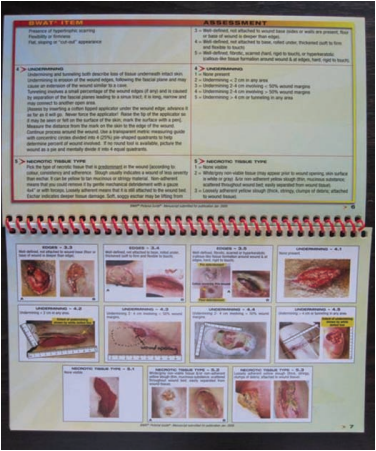
\includegraphics[keepaspectratio, width=8cm]{gambar/panduan_bergambar}
	\caption{Halaman dari panduan bergambar penilaian luka \textit{Bates-Jensen} \citep{sussman2012}}
	\label{gambar:bates_jensen_assessment_tool}
\end{figure}
Luka harus dinilai dengan BWAT pada awalnya untuk penilaian dasar dan secara berkala (yaitu, setidaknya setiap minggu) untuk mengevaluasi efektivitas intervensi.

\section{Penggunaan Skor BWAT untuk Mengidentifikasi Status Keparahan dan Panduan Perawatan}

Tingkat keparahan luka, serta status kesehatan pasien secara keseluruhan, dapat menentukan pendekatan manajemen yang tepat untuk penyembuhan. Status keparahan adalah ukuran derajat kerusakan jaringan atau beban luka pada pasien. Tujuan perawatan luka adalah untuk mengurangi status keparahan secara keseluruhan dan membuat penurunan ini tepat waktu. Perawat dapat menggunakan BWAT untuk membantu perawat mengidentifikasi tingkat keparahan luka, dan dengan demikian memandu perencanaan perawatan pasien.
Seperti yang ditunjukkan pada Gambar 2.2, skor BWAT dapat dibagi menjadi empat status keparahan yang disarankan: skor total 13-20 menunjukkan keparahan minimal; 21–30 menunjukkan keparahan ringan; 31-40 adalah tingkat keparahan sedang; dan 41-65 adalah tingkat keparahan yang ekstrim. Contoh algoritme perawatan untuk satu luka di masing-masing kondisi keparahan ini disajikan di bawah ini. Algoritma pengobatan ini berasal dari pedoman praktek klinis.
\begin{figure}[H]
	\centering
	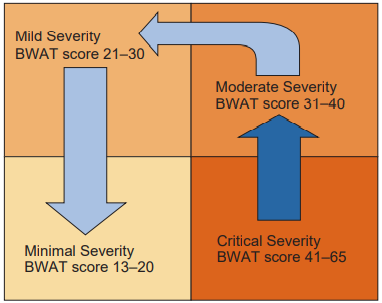
\includegraphics[keepaspectratio, width=8cm]{gambar/skor_tingkat_keparahan}
	\caption{Status keparahan berdasarkan skor BWAT. Tujuan terapi adalah (1) untuk mengurangi tingkat keparahan luka secara keseluruhan dan, dengan demikian, skor BWAT dan (2) untuk membuat penurunan secara tepat waktu. Ada perhatian yang sama mengenai tingkat keparahan luka dan durasi waktu yang dihabiskan luka dalam kondisi parah apa pun. \citep{sussman2012}}
	\label{gambar:skor_tingkat_keparahan_bwat}
\end{figure}
\begin{enumerate}
	\item Skor Tingkat Keparahan Minimal BWAT 13–20
	
	Luka dengan skor total BWAT 13-20 umumnya merupakan luka dengan ketebalan parsial yang dangkal. Gambar 5.23 menyajikan algoritme generik untuk perawatan luka dalam keadaan parah ini. Tujuan utama luka dalam keadaan parah ini adalah untuk mencegah kerusakan lebih lanjut dan menyediakan lingkungan luka yang lembab untuk penyembuhan.
	\item Skor Tingkat Keparahan Ringan BWAT 21–30
	
	Luka dengan tingkat keparahan ringan meliputi luka sebagian dan seluruh ketebalan. Gambar 5.24 menyajikan algoritme perawatan umum untuk luka dengan ketebalan parsial dengan skor keparahan ringan. Tujuan perawatan luka parsial dengan tingkat keparahan ringan adalah untuk menyerap eksudat luka yang berlebihan, mempertahankan dasar luka yang bersih, dan menjaga lingkungan yang lembab. Luka full-thickness dengan skor keparahan ringan menawarkan lebih banyak pilihan untuk pengobatan karena luka dapat muncul sebagai luka bersih, full-thickness atau sebagai luka yang diisi dengan puing-puing nekrotik.
	\item Skor Tingkat Keparahan Sedang BWAT 31–40
	
	Gambar 5.25 adalah rencana perawatan untuk luka full-thickness dengan jaringan nekrotik. Tujuan perawatan luka full-thickness dengan tingkat keparahan sedang adalah untuk mendapatkan/mempertahankan dasar luka yang bersih, menyediakan lingkungan yang lembab, menyerap eksudat berlebih, mencegah penutupan dini, dan mengurangi ruang mati luka. Luka dengan skor keparahan sedang (dan ringan) memiliki presentasi klinis yang paling beragam, sehingga pilihan mengenai pengobatan sangat banyak.
Gambar 5.26 sampai 5.28 menunjukkan algoritma pengobatan umum. Algoritma ini dapat digunakan untuk menentukan perawatan yang tepat untuk berbagai luka kronis dengan skor keparahan BWAT sedang hingga ekstrim. Luka dengan tingkat keparahan sedang sebagian besar merupakan luka full-thickness seperti ulkus dekubitus stadium III atau IV. Gambar 5.26 menyajikan kasus luka full-thickness dengan puing-puing nekrotik dan eksudat dalam jumlah besar. Perawatan difokuskan pada debridement dan penyerapan eksudat. Gambar 5.27 menyajikan kasus luka bersih full-thickness dengan undermining atau dead space, dan fokus pengobatan adalah menghilangkan dead space dan pencegahan penutupan luka prematur. Tujuan perawatan luka pada keadaan keparahan ini adalah untuk mendapatkan/mempertahankan dasar luka yang bersih, menyerap eksudat berlebih, menghilangkan ruang mati untuk mencegah penutupan luka prematur, dan menyediakan lingkungan luka yang lembab.
	\item Skor Tingkat Keparahan Kritis BWAT 41–65
	
	Luka dengan skor total BWAT antara 41 dan 65 umumnya merupakan luka full-thickness yang dalam dengan manifestasi klinis yang lebih kritis, termasuk undermining dan nekrosis. Gambar 5.28 menyajikan algoritma untuk perawatan luka dengan eskar nekrotik. Tujuan perawatan luka pada keadaan keparahan ini adalah untuk mengidentifikasi dan mengobati infeksi, mendapatkan dasar luka yang bersih, menyerap eksudat berlebih, menghilangkan ruang mati untuk mencegah penutupan luka prematur, dan menyediakan lingkungan luka yang lembab.
Pertimbangan dalam Menggunakan Skor BWAT untuk Memandu Perawatan
Penggunaan skor BWAT untuk menentukan keadaan keparahan dan membimbing pengobatan menawarkan satu pendekatan untuk mengelola luka. Pendekatan ini mungkin berguna dalam merancang pedoman pengobatan generik yang luas; namun, pasien tetap harus menggunakan penilaian klinis perawat untuk mengindividualisasikan rencana perawatan. Selain itu, rencana perawatan yang disajikan berdasarkan skor keparahan BWAT hanya berfokus pada perawatan luka topikal. Perhatian pada nutrisi, penggunaan permukaan penopang yang memadai, penentuan kebutuhan perawatan luka yang lebih lanjut, dan pertimbangan status seluruh pasien juga merupakan bagian dari rencana perawatan.
\end{enumerate}
\begin{figure}[H]
	\centering
	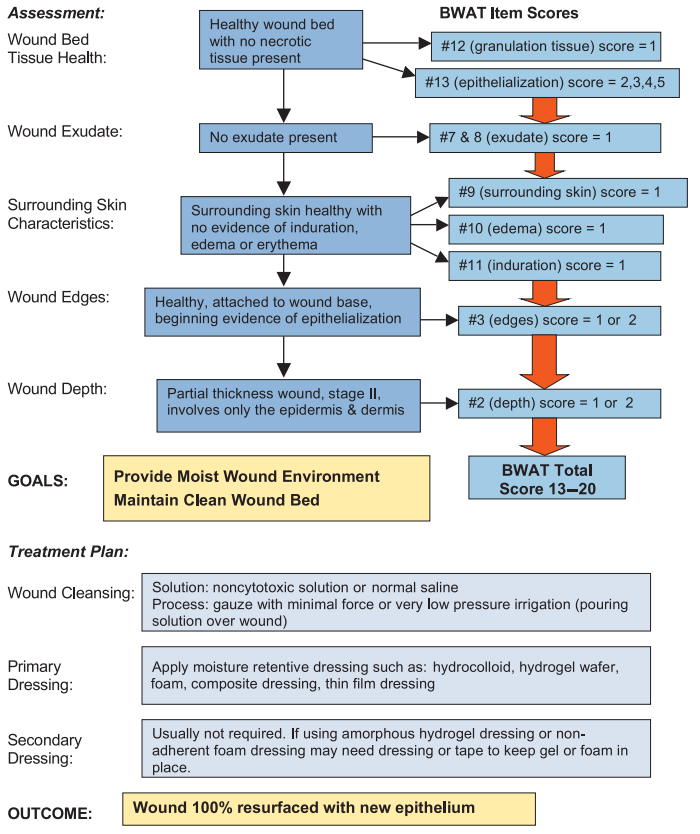
\includegraphics[keepaspectratio, width=14cm]{gambar/gambar_23}
	\caption{Algoritma perawatan skor keparahan BWAT minimal untuk luka ringan, kering, dengan ketebalan sebagian. (Diadaptasi dari ConvaTec, dengan izin.) \citep{sussman2012}}
	\label{gambar:gambar_23}
\end{figure}

\begin{figure}[H]
	\centering
	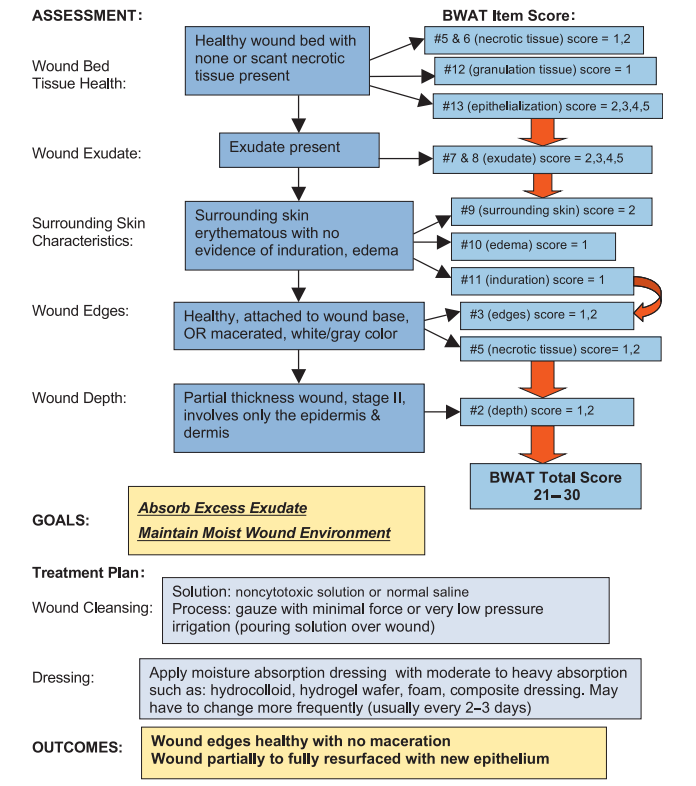
\includegraphics[keepaspectratio, width=14cm]{gambar/gambar_24}
	\caption{Parsial-ketebalan luka dengan algoritma pengobatan skor keparahan BWAT ringan. (Diadaptasi dari ConvaTec, dengan izin.) \citep{sussman2012}}
	\label{gambar:gambar_24}
\end{figure}

\begin{figure}[H]
	\centering
	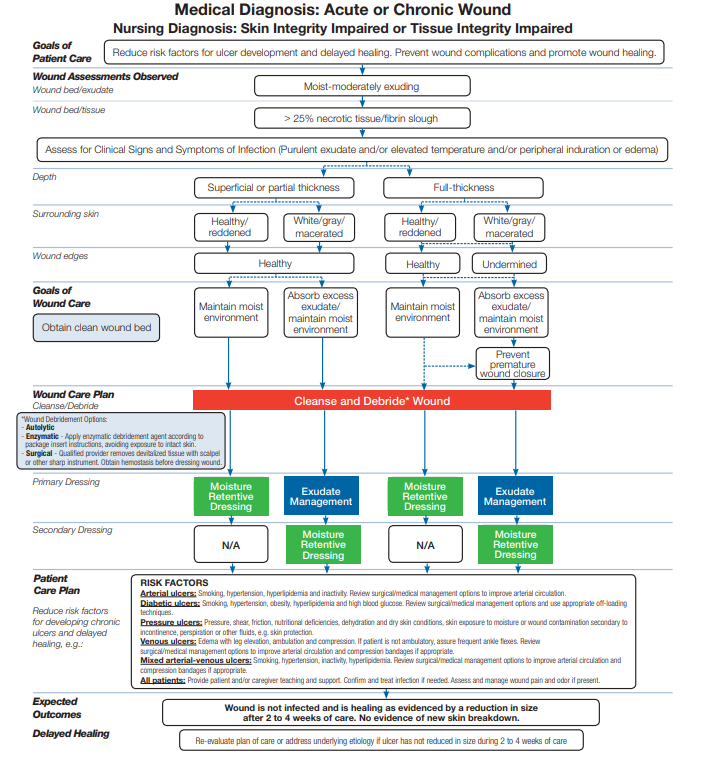
\includegraphics[keepaspectratio, width=14cm]{gambar/gambar_25}
	\caption{Ulkus tekan stadium III atau stadium IV dengan ketebalan penuh dengan algoritme pengobatan skor keparahan BWAT sedang. (Diadaptasi dari ConvaTec, dengan izin.) \citep{sussman2012}}
	\label{gambar:gambar_25}
\end{figure}

\begin{figure}[H]
	\centering
	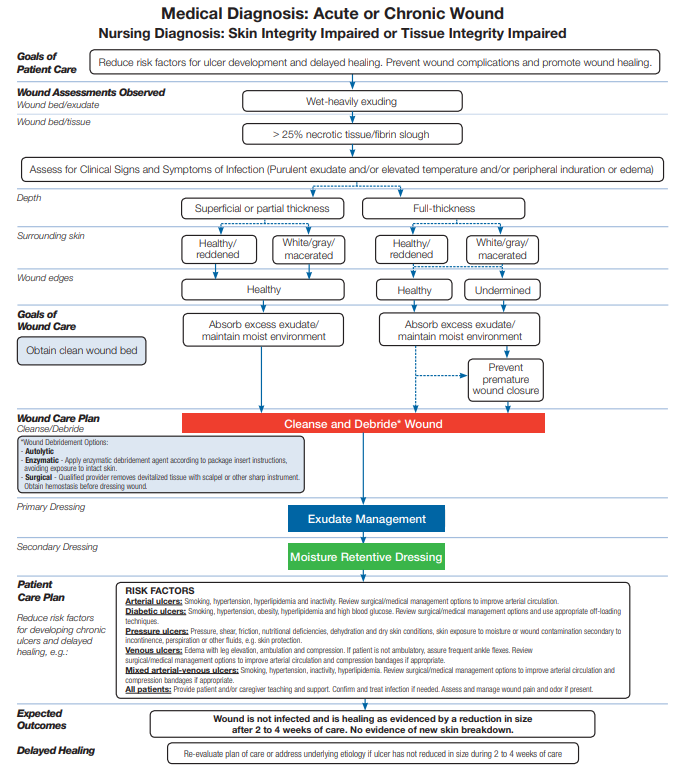
\includegraphics[keepaspectratio, width=14cm]{gambar/gambar_26}
	\caption{Luka dengan ketebalan penuh umum dengan algoritme perawatan skor keparahan BWAT kritis. (Dicetak ulang dari ConvaTec, dengan izin.) \citep{sussman2012}}
	\label{gambar:gambar_26}
\end{figure}

\begin{figure}[H]
	\centering
	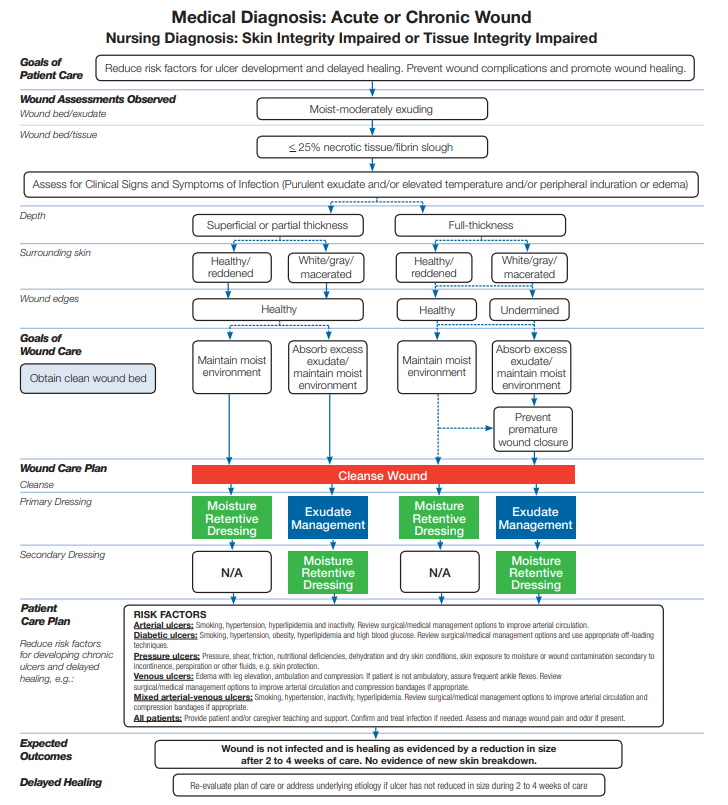
\includegraphics[keepaspectratio, width=14cm]{gambar/gambar_27}
	\caption{Luka dengan ketebalan penuh umum dengan \textit{undermining} atau \textit{pocketing} dengan algoritme perawatan skor keparahan BWAT sedang. (Dicetak ulang dari ConvaTec, dengan izin.) \citep{sussman2012}}
	\label{gambar:gambar_27}
\end{figure}

\begin{figure}[H]
	\centering
	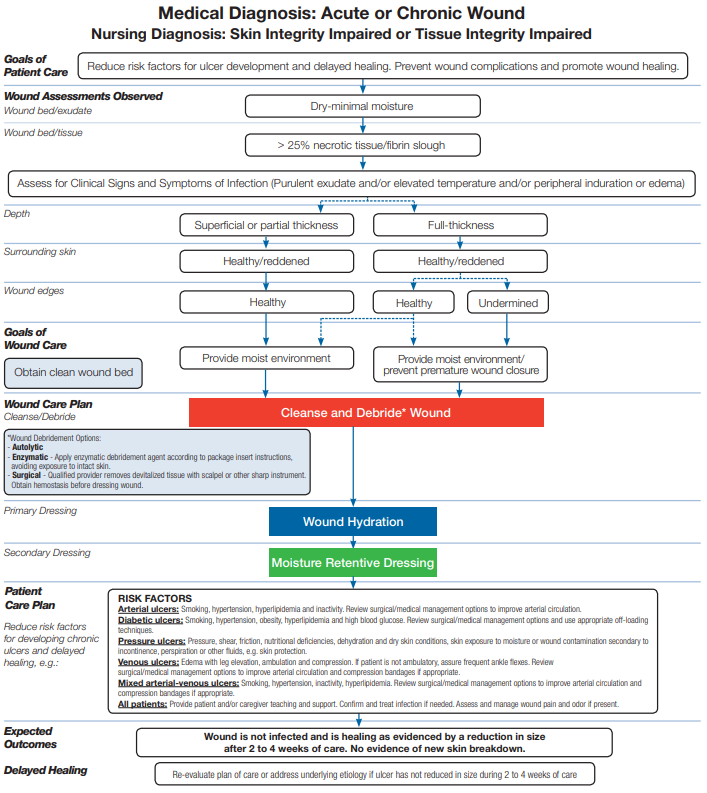
\includegraphics[keepaspectratio, width=14cm]{gambar/gambar_28}
	\caption{Skor keparahan BWAT kritis dengan algoritme perawatan eschar kering. (Dicetak ulang dari ConvaTec, dengan izin.) \citep{sussman2012}}
	\label{gambar:gambar_28}
\end{figure}

\section{\emph{Activity vs Fragment}}

\emph{Activity} adalah satu hal yang terfokus dapat dilakukan pengguna. Hampir semua \textit{activity} berinteraksi dengan pengguna, jadi \textit{class Activity} menangani pembuatan desain untuk menempatkan \textit{User Interface}(UI) dengan \textit{setContentView(View)}.
\textit{Fragment} mewakili bagian UI aplikasi yang dapat digunakan kembali. \textit{Fragment} mendefinisikan dan mengelola tata letaknya sendiri, memiliki siklus hidupnya sendiri, dan dapat menangani kejadian \textit{input}nya sendiri. \textit{Fragment} tidak dapat hidup sendiri, harus di\textit{hosting} oleh \textit{activity} atau \textit{fragment} lain.
Perbedaan utama yang muncul dari definisi di atas adalah bahwa \textit{fragment} bergantung pada \textit{activity} yang ada sehingga hanya mewakili sebagian UI. Sebaliknya, \textit{activity} dapat dianggap seperti wadah dimana semua komponen UI lainnya (termasuk \textit{fragment}) akan ditempatkan. Tanpa \textit{activity}, tidak akan ada \textit{interface} pengguna. Cara untuk membuat \textit{fragment} ialah:
\begin{enumerate}
\item \textit{Setup environment}

Fragment memerlukan dependency pada library AndroidX Fragment. Diperlukan menambahkan repositori Google Maven ke file settings.gradle proyek untuk menyertakan dependency
\begin{figure}[H]
	\centering
	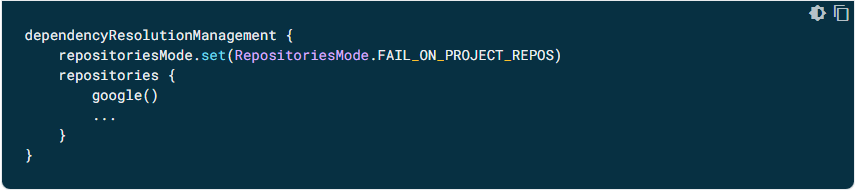
\includegraphics[keepaspectratio, width=12cm]{gambar/fragment_setup_environment1}
	\caption{Contoh menambahkan repositori \textit{Google Maven} pada \textit{dependency} \citep{developerandroid}}
	\label{gambar:gambar_29}
\end{figure}
Untuk menyertakan \textit{AndroidX Fragment} ke proyek, tambahkan \textit{dependency} berikut dalam file \textit{build.gradle}:
\begin{figure}[H]
	\centering
	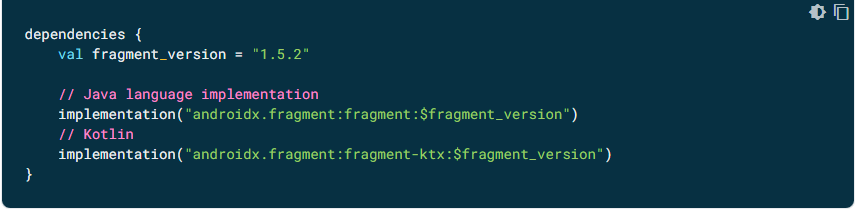
\includegraphics[keepaspectratio, width=12cm]{gambar/fragment_setup_environment2}
	\caption{Contoh menambahkan \textit{AndroidX Fragment} \citep{developerandroid}}
	\label{gambar:gambar_30}
\end{figure}
\item Buat kelas \emph{fragment}

Untuk membuat \textit{fragment}, perluas kelas \textit{AndroidX Fragment}, dan ganti metodenya untuk menyisipkan logika aplikasi, mirip dengan cara membuat kelas \textit{Activity}. Untuk membuat \textit{fragment} minimal yang menentukan \textit{layout}nya sendiri, berikan \textit{resource layout fragment} ke konstruktor dasar, contohnya sebagai berikut:
\begin{figure}[H]
	\centering
	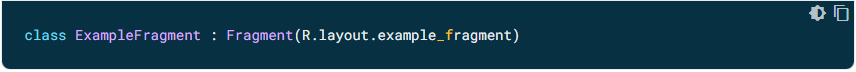
\includegraphics[keepaspectratio, width=12cm]{gambar/fragment_class}
	\caption{Contoh berikan \textit{resource layout fragment} ke konstruktor dasar \citep{developerandroid}}
	\label{gambar:gambar_31}
\end{figure}
\textit{Library fragment} juga menyediakan kelas dasar \textit{fragment} yang lebih khusus:
	\begin{enumerate}
	\item \emph{DialogFragment}
	
	Menampilkan dialog mengambang. Menggunakan kelas ini untuk membuat dialog adalah alternatif yang baik untuk menggunakan metode pembantu dialog di kelas Activity, karena fragment secara otomatis menangani pembuatan dan pembersihan dialog.
	\item \emph{PreferenceFragmentCompat}
	
	Menampilkan hierarki objek \textit{Preference} sebagai daftar. Kita dapat menggunakan \textit{PreferenceFragmentCompat} untuk membuat layar pengaturan untuk aplikasi.
	\end{enumerate}
\item Tambahkan \textit{fragment} ke \textit{activity}

Umumnya, \textit{fragment} harus disematkan dalam \textit{AndroidX FragmentActivity} untuk menyumbangkan UI ke \textit{layout activity} tersebut. \textit{FragmentActivity} adalah kelas dasar untuk \textit{AppCompatActivity}, jadi jika sudah membuat subkelas \textit{AppCompatActivity} maka tidak perlu mengubah kelas dasar \textit{activity}.
Kita dapat menambahkan \textit{fragment} ke hierarki \textit{view activity} baik dengan mendefinisikan \textit{fragment} di file \textit{layout activity} atau dengan mendefinisikan wadah \textit{fragment} di file \textit{layout activity}, lalu menambahkan \textit{fragment} secara terprogram dari dalam \textit{activity}. Dalam kedua kasus tersebut, kita perlu menambahkan \textit{FragmentContainerView} yang menentukan lokasi tempat \textit{fragment} harus ditempatkan dalam hierarki \textit{view activity}. Sangat disarankan untuk selalu menggunakan \textit{FragmentContainerView} sebagai wadah untuk gragment, karena \textit{FragmentContainerView} menyediakan perbaikan khusus untuk \textit{fragment} yang tidak disediakan oleh grup \textit{view} lain seperti \textit{FrameLayout}.
	\begin{enumerate}
	\item Menambahkan \textit{fragment} melalui \textit{XML}
	
	Untuk menambahkan fragment secara deklaratif ke XML layout activity, gunakan elemen FragmentContainerView seperti berikut:
\begin{figure}[H]
	\centering
	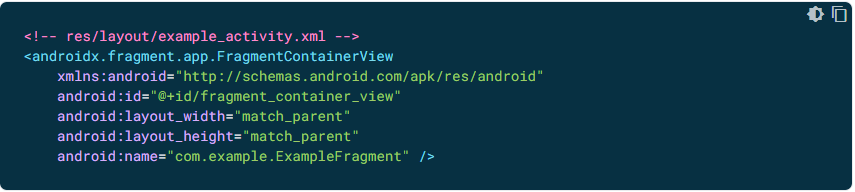
\includegraphics[keepaspectratio, width=12cm]{gambar/fragment_add}
	\caption{Contoh \textit{FragmentContainerView} pada \textit{XML} \citep{developerandroid}}
	\label{gambar:gambar_32}
\end{figure}
	Atribut \textit{android:name} menentukan nama kelas \textit{Fragment} yang akan dibuat \textit{instance}-nya. Saat \textit{layout activity} di-\textit{inflate}, \textit{fragment} yang ditentukan akan dibuat \textit{instance}-nya, \textit{onInflate}() dipanggil pada \textit{fragment} yang baru dibuat \textit{instance}-nya, dan \textit{FragmentTransaction} dibuat untuk menambahkan \textit{fragment} ke \textit{FragmentManager}.
	\item Menambahkan \textit{fragment} secara terprogram
	
	Untuk menambahkan \textit{fragment} secara terprogram ke \textit{layout activity}, \textit{layout} harus menyertakan \textit{FragmentContainerView} yang berfungsi sebahai wadah \textit{fragment}, seperti yang ditunjukkan dalam contoh berikut:
\begin{figure}[H]
	\centering
	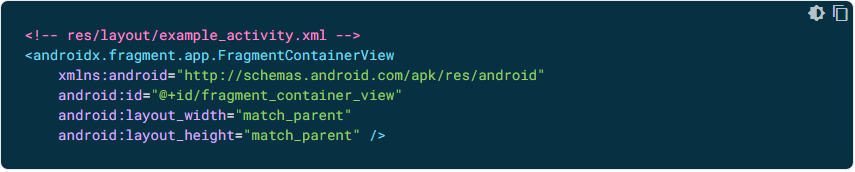
\includegraphics[keepaspectratio, width=12cm]{gambar/fragment_add1}
	\caption{Contoh menambahkan \textit{fragment} secara terprogram. \citep{developerandroid}}
	\label{gambar:gambar_33}
\end{figure}
	Tidak seperti pendekatan \textit{XML}, atribut \textit{android:name} tidak digunakan pada \textit{FragmentContainerView} di sini, jadi tidak ada \textit{fragment} tertentu yang dibuat secara otomatis. Sebagai gantinya, \textit{FragmentTransaction} digunakan untuk membuat \textit{instance fragment} dan menambahkannya ke \textit{layout activity}
	\end{enumerate}
Saat \textit{activity} berjalan, kita dapat melakukan transaksi \textit{fragment} seperti menambahkan, menghapus, atau mengganti \textit{fragment}. Di \textit{FragmentActivity}, kita bisa mendapatkan \textit{instance FragmentManager}, yang dapat digunakan untuk membuat \textit{FragmentTransaction}. Kemudian, kita bisa membuat \textit{instance fragment} dalam metode \textit{onCreate}() \textit{activity} menggunakan \textit{FragmentTransaction.add}(), meneruskan \textit{ID ViewGroup} dari \textit{container} di \textit{layout} dan kelas \textit{fragment} yang ingin ditambahkan, lalu kemudian melakukan transaksi, seperti yang ditunjukkan dalam contoh berikut:
\begin{figure}[H]
	\centering
	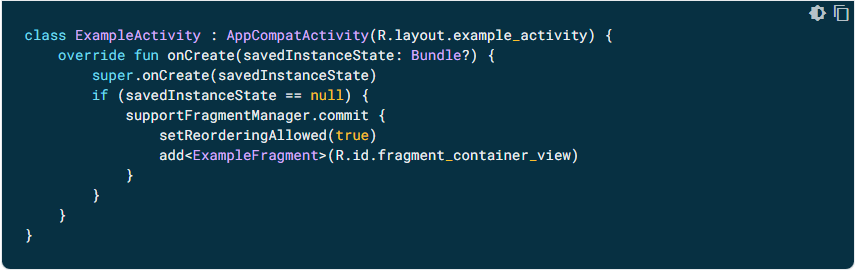
\includegraphics[keepaspectratio, width=12cm]{gambar/fragment_add2}
	\caption{Contoh membuat \textit{FragmentTransaction}. \citep{developerandroid}}
	\label{gambar:gambar_34}
\end{figure}
Pada contoh sebelumnya, perhatikan bahwa transaksi \textit{fragment} hanya dibuat ketika \textit{storedInstanceState} adalah \textit{null}. Ini untuk memastikan bahwa \textit{fragment} hanya ditambahkan sekali, saat \textit{activity} pertama kali dibuat. Saat terjadi perubahan konfigurasi dan \textit{activity} dibuat ualng, \textit{saveInstanceState} tidak lagi \textit{null}, dan \textit{fragment} tidak perlu ditambahkan untuk kedua kalinya, karena \textit{fragment} secara otomatis dipulihkan dari \textit{saveInstanceState}.
Jika \textit{fragment} memerlukan beberapa data awal, argumen dapat diteruskan ke \textit{fragment} dengan menyediakan \textit{bundle} dalam panggilan ke \textit{FragmentTransaction.add}(), seperti yang ditunjukkan di bawah ini:
\begin{figure}[H]
	\centering
	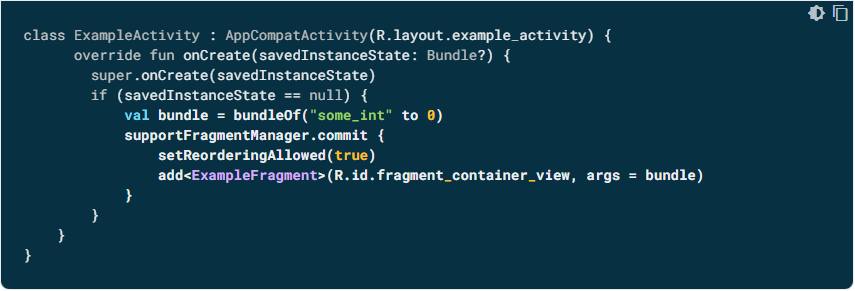
\includegraphics[keepaspectratio, width=12cm]{gambar/fragment_add3}
	\caption{Contoh menambahkan beberapa data awal. \citep{developerandroid}}
	\label{gambar:gambar_35}
\end{figure}
\textit{Bundle} argumen kemudian dapat diambil dari dalam \textit{fragment} dengan memanggil \textit{requireArgument}(), dan metode pengambil \textit{bundle} yang sesuai dapat digunakan untuk mengambil setiap argumen.
\begin{figure}[H]
	\centering
	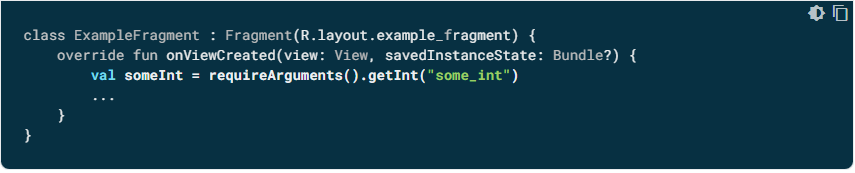
\includegraphics[keepaspectratio, width=12cm]{gambar/fragment_add4}
	\caption{Contoh memanggil \textit{requireArgmunet}(). \citep{developerandroid}}
	\label{gambar:gambar_36}
\end{figure}
\end{enumerate}

\section{\emph{Navigation} dan \emph{menu}}

Navigation mengacu pada interaksi yang memungkinkan pengguna bernavigasi melintasi, masuk, dan mundur dari berbagai bagian konten dalam aplikasi. Komponen navigation dalam Android membantu menerapkan navigasi mulai dari klik tombol sederhana hingga pola yang lebih kompleks, seperti bilah aplikasi dan panel samping navigasi. Komponen navigation juga memastikan pengalaman pengguna yang konsisten dan dapat diprediksi dengan mengikuti serangkaian prinsip yang telah ditetapkan.
Komponen navigation terdiri dari tiga bagian penting:
\begin{enumerate}
\item{\textit{Navigation graph}: sumber daya \textit{XML} yang berisi semua informasi terkait navigasi di satu lokasi terpusat. Ini mencakup semua area konten individual dalam aplikasi, yang disebut \textit{destinations}, serta kemungkinan jalur yang dapat diambil \textit{user} melalui aplikasi.}
\item{\textit{NavHost}: wadah kosong yang menampilkan tujuan dari \textit{navigation graph}. Komponen \textit{navigation} berisi implementasi \textit{default NavHost}, \textit{NavHostFragment}, yang menampilkan tujuan \textit{fragment}.}
\item{\textit{NavController}: objek yang mengelola navigasi aplikasi dalam \textit{NavHost}. \textit{NavController} mengatur pertukaran konten tujuan di \textit{NavHost} saat \textit{user} bergerak di seluruh aplikasi.}
\end{enumerate}

Saat menavigasi melalui aplikasi, kita memberi tahu \textit{NavController} bahwa kita ingin menavigasi di sepanjang jalur tertentu dalam \textit{Navigation graph} atau langsung ke tujuan tertentu. \textit{NavController} kemudian menunjukkan tujuan yang sesuai di \textit{NavHost}. Komponen \textit{navigation} memberikan sejumlah manfaat lain sebagai berikut:

\begin{enumerate}
\item Menangani transaksi fragment.
\item Menangani action up dan action back dengan benar secara default.
\item Menyediakan sumber daya standar untuk animasi dan transisi.
\item Menerapkan dan menangani deep linking.
\item Termasuk pola navigasi UI, seperti panel samping navigasi dan navigasi bawah, dengan sedikit pekerjaan tambahan.
\item Safe Args – plugin Gradle yang menyediakan keamanan jensi saat menavigasi dan meneruskan data antar tujuan.
\item Dukungan ViewModel – kita dapat memasukkan ViewModel ke navigation graph untuk berbagi data terkait UI di antara destination graph.
\item Selain itu juga dapat menggunakan editor navigasi android studio untuk melihat dan mengedit navigation graph.
\end{enumerate}

Cara untuk menggunakan \textit{navigation} adalah sebagai berikut:
\begin{enumerate}
\item \textit{Setup environment}

Untuk menyertakan dukungan \textit{Navigation} dalam proyek, tambahkan dependensi berikut ke file \textit{build.gradle} aplikasi:
\begin{figure}[H]
	\centering
	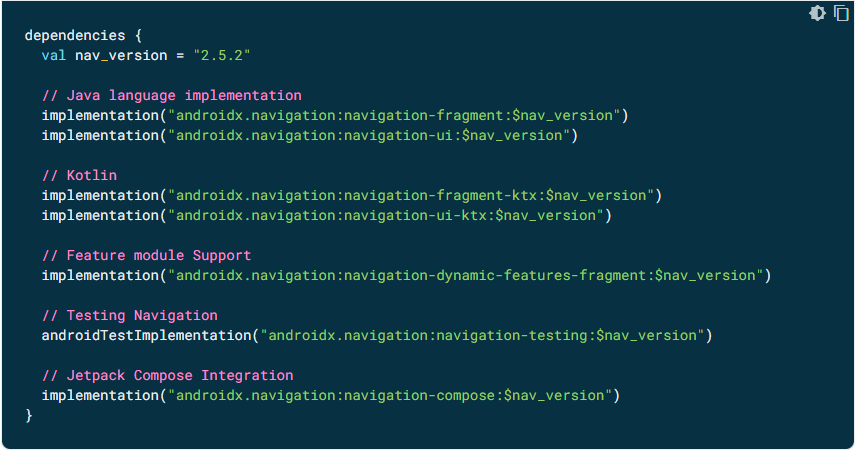
\includegraphics[keepaspectratio, width=12cm]{gambar/navigation_setup}
	\caption{Contoh dependensi untuk \textit{navigation} \citep{developerandroid}}
	\label{gambar:gambar_37}
\end{figure}

\item Buat \emph{navigation graph}

Navigasi terjadi di antara tujuan aplikasi, dimana saja di aplikasi yang dapat dinavigasi oleh pengguna. Tujuan ini terhubung melalui tindakan. \textit{Navigation graph} adalah \textit{file resource} yang berisi semua tujuan dan tindakan. \textit{Graph} mewakili semua jalur \textit{navigation} aplikasi.

Gambar 1 menunjukkan representasi visual \textit{graph navigation} untuk aplikasi sampel yang berisi enam tujuan yang dihubungkan oleh lima tindakan. Setiap tujuan diwakili oleh gambar mini pratinjau, dan tindakan menghubungkan diwakili oleh panah yang menunjukkan bagaimana pengguna dapat menavigasi dari satu tujuan ke tujuan lainnya.
\begin{figure}[H]
	\centering
	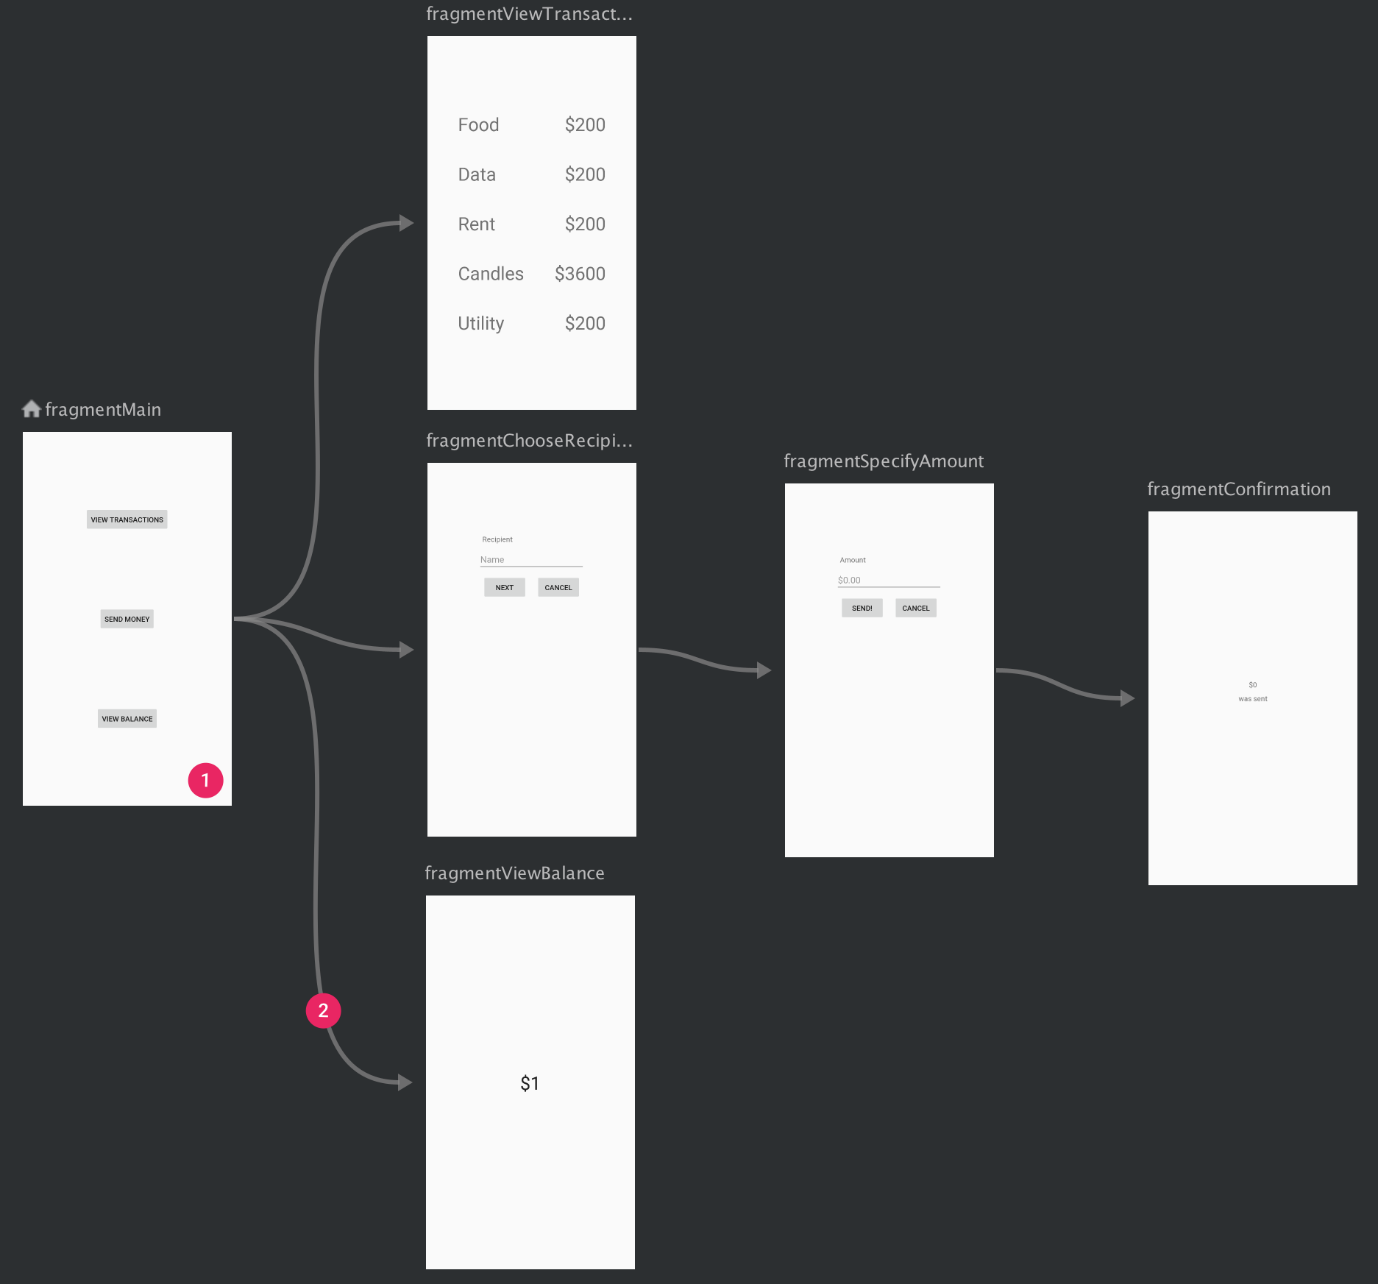
\includegraphics[keepaspectratio, width=12cm]{gambar/navigation_graph1}
	\caption{Grafik navigasi yang menampilkan pratinjau dari enam tujuan berbeda yang terhubung melalui lima tindakan \citep{developerandroid}}
	\label{gambar:gambar_38}
\end{figure}

	\begin{enumerate}
	\item \textit{Destinations} adalah area konten yang berbeda di aplikasi.
	\item \textit{Actions} adalah koneksi logis antara tujuan yang mewakili jalur yang dapat diambil pengguna.
	\end{enumerate}
	
Untuk menambahkan \textit{graph navigation} ke proyek adalah sebagai berikut:
	\begin{enumerate}
	\item Di jendela \textit{project}, klik kanan pada direktori \textit{res} dan pilih \textit{New} > \textit{Android Resource File}. Dialog \textit{file resource} baru muncul.
	\item Ketik nama di \textit{field} nama \textit{file}, seperti \textit{$"nav_graph"$}.
	\item Pilih navigasi dari daftar \textit{drop-down} jenis \textit{resource}, lalu klik \textit{Ok}.
	\end{enumerate}
	
Ketika menambahkan \textit{graph navigation} pertama, \textit{Android Studio} membuat direktori \textit{resource navigation} di dalam direktori \textit{res}. Direktori ini berisi \textit{file resource graph navigation} (\textit{$nav_graph.xml$}, misalnya).

\item \emph{Navigation editor}

Setelah menambahkan \textit{graph}, \textit{Android Studio} membuka \textit{frap} di \textit{Navigation Editor}. Di sini dapat mengedit \textit{navigation graph} secara visual atau langsung mengedit \textit{XML} yang mendasarinya.
\begin{figure}[H]
	\centering
	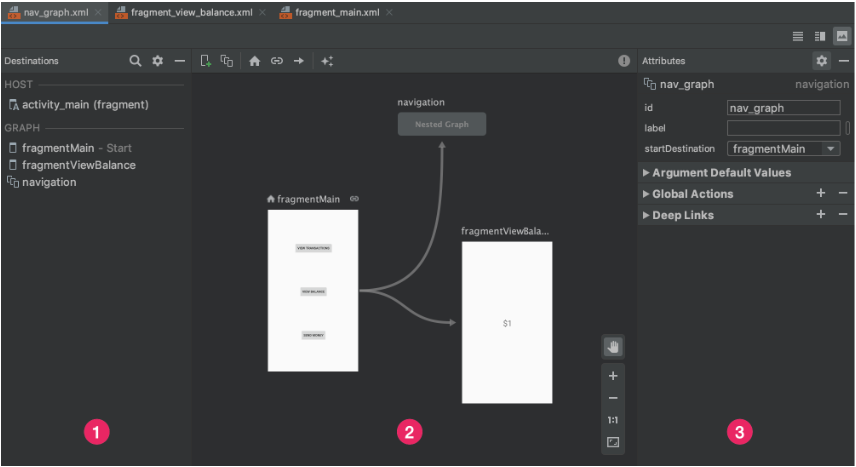
\includegraphics[keepaspectratio, width=12cm]{gambar/navigation_graph2}
	\caption{\textit{Navigation Editor} \citep{developerandroid}}
	\label{gambar:gambar_39}
\end{figure}

	\begin{enumerate}
	\item \textit{Destinations panel}: mencantumkan \textit{host} navigasi dan semua tujuan yang saat ini ada di \textit{Graph Editor}.
	\item 	\textit{Graph Editor}: berisi representasi visual dari \textit{navigation graph}. Dapat beralih antara tampilan desain dan representasi \textit{XML} yang mendasarinya dalam tampilan teks.
	\item \textit{Attributes}: menampilkan atribut untuk item yang saat ini dipilih dalam \textit{navigation graph}.
	\end{enumerate}
	
Klik tab \textit{Text} untuk melihat \textit{XML} yang sesuai, yang akan terlihat mirip dengan gambar berikut:
\begin{figure}[H]
	\centering
	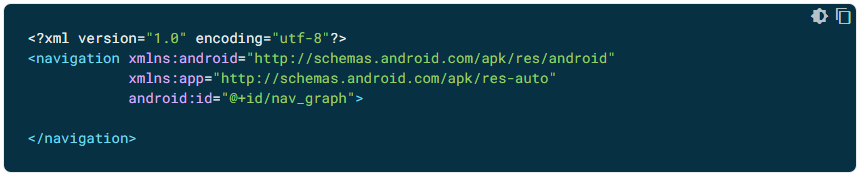
\includegraphics[keepaspectratio, width=12cm]{gambar/navigation_graph3}
	\caption{Contoh \textit{XML navigation graph} \citep{developerandroid}}
	\label{gambar:gambar_40}
\end{figure}

Elemen <\textit{navigation}> adalah elemen \textit{root} dari \textit{navigation graph}. Saat menambahkan tujuan dan menghubungkan tindakan ke \textit{graph}, dapat melihat elemen <\textit{destination}> dan <\textit{action}> yang sesuai di sini sebagai elemen turunan. Jika memiliki \textit{nest graph}, \textit{graph} tersebut muncul sebagai elemen anak <\textit{navigation}>.

\item \emph{Menu}

\textit{Menu} adalah komponen \textit{user interface} yang umum di banyak jenis aplikasi. Untuk memberikan pengalaman pengguna yang familiar dan konsisten harus menggunakan \textit{menu API} untuk menyajikan \textit{user action} dan opsi lain dalam \textit{activity}.

Mulai \textit{android} 3.0, perangkat yang diberdayakan android tidak lagi diharuskan menyediakan tombol \textit{menu} khusus. Dengan perubahan ini, aplikasi android harus bermigrasi dari ketergantungan pada panel menu 6 item tradisional dan sebagai gantinya menyediakan bilah aplikasi untuk menyajikan tindakan pengguna yang umum.

Meskipun desan dan pengalaman pengguna untuk beberapa \textit{item menu} telah berubah, semantik untuk menentukan serangkaian tindakan dan opsi masih didasarkan pada \textit{menu API}. Cara membuat tiga tipe dasar \textit{menu}: \textit{Options menu and app bar}, \textit{Context menu and contextual action mode}, \textit{Popup menu}.

Untuk semua jenis \textit{menu}, Android menyediakan format \textit{XML} standar untuk mendefinisikan \textit{item menu}. Alih-alih membuat \textit{menu} dalam kode \textit{aktivitas}, kita harus mendefinisikan \textit{menu} dan semua itemnya dalam sumber data \textit{menu XML}. Anda kemudian dapat mengembang sumber daya menu (memuatnya sebagai objek Menu) di \textit{activity} atau \textit{fragment}.

Menggunakan menu resource adalah praktik yang baik karena beberapa alasan:
	\begin{enumerate}
	\item Lebih mudah untuk memvisualisasikan struktur \textit{menu} dalam \textit{XML}.
	\item Ini memisahkan konten untuk \textit{menu} dari \textit{applications behavioral code}.
	\item Ini memungkinkan membuat konfigurasi \textit{menu} alternatif untuk berbagai versi platform, ukuran layar, dan konfigurasi lainnya dengan memanfaatkan \textit{framework} aplikasi.
	\end{enumerate}

Untuk menentukan menu, buat file XML di dalam direktori res/menu/ dan buat menu dengan elemen berikut:
	\begin{enumerate}
	\item 1.	<\textit{menu}> = Mendefinisikan menu, yang merupakan wadah untuk \textit{item menu}. Elemen <\textit{menu}> harus menjadi simpul akar untuk \textit{file} dan dapat menampung satu atau lebih elemen <\textit{item}> dan <\textit{group}>.
	\item <\textit{item}> = Membuat \textit{menu item}, yang mewakili satu \textit{item} dalam \textit{menu}. Elemen ini mungkin berisi elemen sarang <\textit{menu}> yang membuat \textit{submenu}.
	\item <\textit{group}> = Wadah opsional yang tidak terlihat untuk elemen <\textit{item}>. Ini memungkinkan untuk mengkategorikan \textit{item menu} sehingga mereka berbagi properti seperti status aktif dan visibilitas.
	\end{enumerate}

Berikut contoh menu bernama $game_menu.xml$:
\begin{figure}[H]
	\centering
	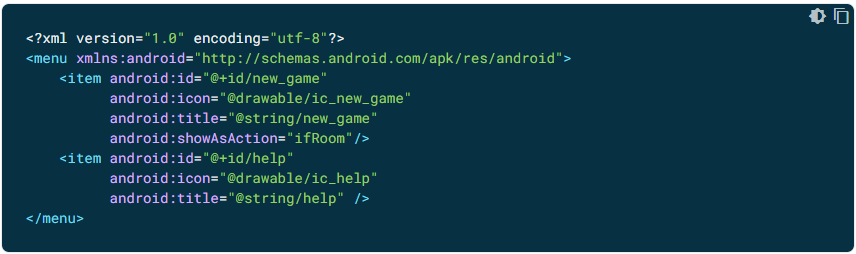
\includegraphics[keepaspectratio, width=12cm]{gambar/menu}
	\caption{Contoh \textit{menu} \citep{developerandroid}}
	\label{gambar:gambar_41}
\end{figure}

Elemen <\textit{item}> mendukung beberapa atribut yang dapat digunakan untuk menentukan tampilan dan perilaku item. \textit{Item} dalam \textit{menu} di atas mencakup atribut berikut:
	\begin{enumerate}
	\item \textit{android:id} = \textit{ID resource} yang unik untuk \textit{item}, yang memungkinkan aplikasi mengenali \textit{item} saat pengguna memilihnya.
	\item \textit{android:icon} = Referensi ke \textit{resource} gambar untuk digunakan sebagai ikon \textit{item}.
	\item \textit{android:title} = referensi ke \textit{string} untuk digunakan sebagai judul \textit{item}.
	\item \textit{android:showAsAction} = Menentukan kapan dan bagaimana \textit{item} ini akan muncul sebagai \textit{item} tindakan di bilah aplikasi.
	\end{enumerate}
Ini adalah atribut terpenting yang harus digunakan, tetapi masih banyak lagi yang tersedia.
\end{enumerate}

\section{Layouting}

Layout mendefinisikan struktur untuk user interface di aplikasi, seperti dalam suatu aktivitas. Semua elemen dalam layout dibangun menggunakan hierarki objek View dan ViewGroup. View biasanya menggambar sesuatu yang dapat dilihat dan berinteraksi dengan pengguna. Sedangkan ViewGroup adalah wadah tak terlihat yang mendefinisikan struktur layout untuk View dan objek ViewGroup lainnya.
\begin{figure}[H]
	\centering
	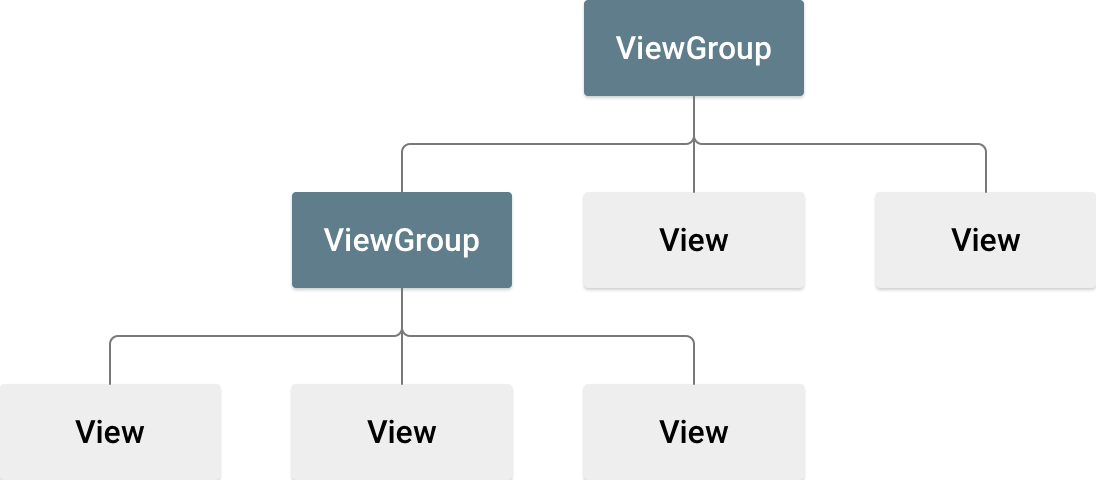
\includegraphics[keepaspectratio, width=12cm]{gambar/layout_hirarki}
	\caption{Ilustrasi hierarki tampilan, yang menentukan tata letak UI \citep{developerandroid}}
	\label{gambar:gambar_42}
\end{figure}

Objek \textit{View} biasanya disebut "\textit{widget}" dan bisa menjadi salah satu dari banyak \textit{subclass}, seperti \textit{Button} atau \textit{TextView}. Objek \textit{ViewGroup} biasanya disebut "\textit{layout}" dapat menjadi salah satu dari banyak jenis yang menyediakan struktur \textit{layout} yang berbeda, seperti \textit{LinearLayout} atau \textit{ConstraintLayout}. Deklarasi \textit{layout} dapat dengan dua cara:
\begin{enumerate}
\item Deklarasikan elemen UI dalam \textit{XML}. 

Android menyediakan kosakata \textit{XML} langsung yang sesuai dengan kelas dan subkelas \textit{View}, seperti untuk \textit{widget} dan \textit{layout}. Kita juga dapat menggunakan \textit{layout} editor android studio untuk membangun \textit{layout XML} menggunakan \textit{interface} \textit{“drag-and-drop”}.
\item Buat \textit{instance} elemen \textit{layout} saat \textit{runtime}. 

Aplikasi kita dapat membuat objek \textit{View} dan \textit{ViewGroup} (dan memanipulasi propertinya) secara terprogram.
\end{enumerate}

Mendeklarasikan UI dalam \textit{XML} memungkinkan kita untuk memisahkan presentasi aplikasi dari kode yang mengontrol perilakunya. Menggunakan file \textit{XML} juga memudahkan untuk menyediakan \textit{layout} yang berbeda untuk ukuran dan orientasi layar yang berbeda.
Kerangka kerja android memberi kita fleksibilitas untuk menggunakan salah satu atau kedua metode ini untuk membangun UI aplikasi. Misalnya bisa mendeklarasikan \textit{layout default} aplikasi dalam \textit{XML}, lalu memodifikasi \textit{layout} saat waktu proses.

Dengan menggunakan kosakata \textit{XML} Android, kita dapat dengan cepat mendesain tata letak UI dan elemen layar yang dikandungnya dengan cara yang sama seperti membuat halaman web dalam \textit{HTML} dengan serangkaian elemen bersarang.

Setiap \textit{file layout} harus berisi tepat satu elemen \textit{root} yang harus berupa objek \textit{View} atau \textit{ViewGroup}. Setelah menentukan elemen \textit{root}, dapat menambahkan objek atau \textit{widget layout} tambahan sebagai elemen turunan untuk membangun hierarki \textit{View} yang mendefinisikan \textit{layout} secara bertahap. Contohnya ini \textit{layout XML} yang menggunakan \textit{LinearLayout} vertikal untuk menampung \textit{TextView} dan \textit{Button}:
\begin{figure}[H]
	\centering
	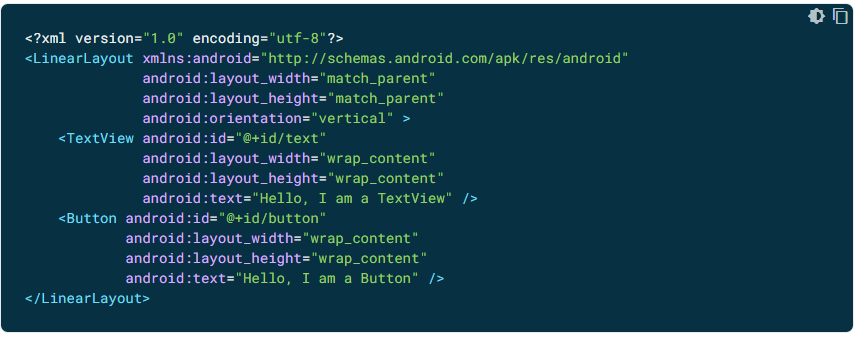
\includegraphics[keepaspectratio, width=12cm]{gambar/layout_linearlayout}
	\caption{Contoh \textit{layout XML} yang menggunakan \textit{LinearLayout} \citep{developerandroid}}
	\label{gambar:gambar_43}
\end{figure}

Setelah dideklarasikan \textit{layout} dalam \textit{XML}, simpan file dengan ekstensi \textit{.xml} di direktori \textit{res/layout/} proyek Android kita sehingga akan dikompilasi dengan benar.

Saat mengompilasi aplikasi, setiap \textit{file layout XML} dikompilasi ke dalam \textit{resource View}. Diharuskan memuat \textit{resource layout} dari kode aplikasi, dalam implementasi \textit{callback Activity.onCreate}(). Lakukan dengan memanggil \textit{setContentView}(), meneruskannya referensi ke \textit{resource layout} dalam bentuk: R\textit{$.layout.layout_file_name$}. Misalnya, jika \textit{layout XML} disimpan sebagai \textit{$main_layout.xml$}, maka akan memuatnya untuk \textit{activity} seperti berikut:
\begin{figure}[H]
	\centering
	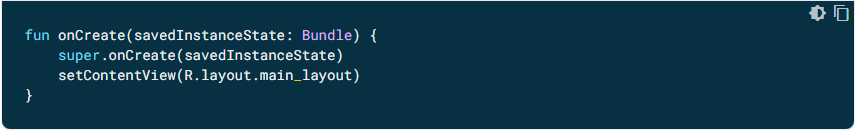
\includegraphics[keepaspectratio, width=12cm]{gambar/layout_setcontentview}
	\caption{Contoh menggunakan \textit{setContentView}() \citep{developerandroid}}
	\label{gambar:gambar_44}
\end{figure}
Metode \textit{callback onCreate}() dalam \textit{activity} dipanggil oleh \textit{framework} Android saat \textit{activity} diluncurkan.
Setiap objek \textit{View} dan \textit{ViewGroup} mendukung berbagai atribut \textit{XML} mereka sendiri. Beberapa atribut khusus untuk objek \textit{View} (misalnya, \textit{TextView} mendukung atribut \textit{textSize}), tetapi atribut ini juga diwarisi oleh objek \textit{View} apa pun yang dapat memperluas kelas ini. Beberapa umum untuk semua objek \textit{View}, karena mereka diwarisi dari kelas \textit{View root} (seperti atribut \textit{id}). Dan, atribut lainnya dianggap sebagai "\textit{parameter layout}", yang merupakan atribut yang menjelaskan orientasi \textit{layout} tertentu dari objek \textit{View}, seperti yang didefinisikan oleh objek induk \textit{ViewGroup} objek tersebut.
Objek \textit{View} apa pun mungkin memiliki \textit{ID integer} yang terkait dengannya, untuk mengidentifikasi \textit{View} secara unik di dalam hierarki. Saat aplikasi dikompilasi, \textit{ID} ini direferensikan sebagai bilangan bulat, tetapi \textit{ID} biasanya ditetapkan dalam \textit{file XML layout} sebagai \textit{string}, dalam atribut \textit{id}. Ini adalah atribut \textit{XML} yang umum untuk semua objek \textit{View} (didefinisikan oleh kelas \textit{View}) dan akan sering digunakan. Sintaks untuk \textit{ID} di dalam \textit{tag XML} adalah:
\begin{figure}[H]
	\centering
	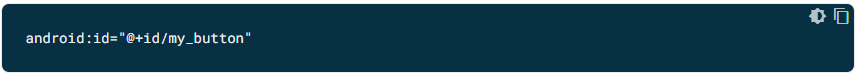
\includegraphics[keepaspectratio, width=12cm]{gambar/layout_tagidbutton}
	\caption{Contoh sintaks untuk \textit{tag ID} \citep{developerandroid}}
	\label{gambar:gambar_45}
\end{figure}
Simbol \textit{(@)} di awal \textit{string} menunjukkan bahwa parser \textit{XML} harus mengurai dan memperluas sisa \textit{string ID} dan mengidentifikasinya sebagai \textit{resource ID}. Tanda tambah (+) berarti bahwa ini adalah nama \textit{resource} baru yang harus dibuat dan ditambahkan ke \textit{resource} kita (dalam \textit{file R.java}). Ada sejumlah \textit{resource ID} lain yang ditawarkan oleh \textit{framework} Android. Saat mereferensikan \textit{ID resource} Android, kita tidak memerlukan simbol tambah, tetapi harus menambahkan \textit{namespace package} Android, seperti:
\begin{figure}[H]
	\centering
	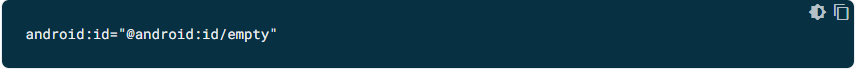
\includegraphics[keepaspectratio, width=12cm]{gambar/layout_tagidbutton2}
	\caption{Contoh menggunakan \textit{namespace package} Android \citep{developerandroid}}
	\label{gambar:gambar_46}
\end{figure}
Dengan \textit{namespace package} Android di tempat, kita sekarang mereferensikan \textit{ID} dari kelas \textit{resource android.R}, bukan dari kelas \textit{resource} lokal.
Untuk membuat View dan mereferensikannya dari aplikasi, pola umumnya adalah:
\begin{enumerate}
\item Tentukan \textit{View}/ \textit{widget} dalam \textit{file layout} dan tetapkan \textit{ID} unik
\begin{figure}[H]
	\centering
	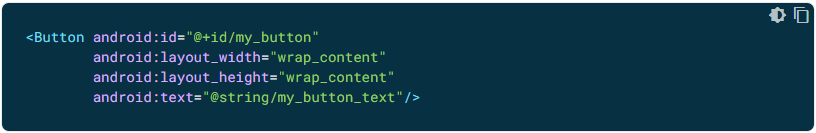
\includegraphics[keepaspectratio, width=12cm]{gambar/layout_view1}
	\caption{Menetapkan \textit{ID} unik \citep{developerandroid}}
	\label{gambar:gambar_47}
\end{figure}
\item Kemudian buat \textit{instance} objek \textit{view} dan ambil dari \textit{layout} (biasanya dalam metode \textit{onCreate}())
\begin{figure}[H]
	\centering
	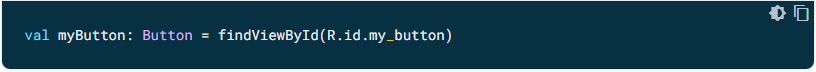
\includegraphics[keepaspectratio, width=12cm]{gambar/layout_view2}
	\caption{Membuat \textit{instance} objek \textit{view} \citep{developerandroid}}
	\label{gambar:gambar_48}
\end{figure}
\end{enumerate}
Mendefinisikan \textit{ID} untuk objek \textit{view} penting saat membuat \textit{RelativeLayout}. Dalam \textit{RelativeLayout}, \textit{view} dapat menentukan \textit{layout}nya relatif terhadap tampilan \textit{view} lainya, yang direferensikan oleh \textit{ID} unik. \textit{ID} tidak harus unik diseluruh \textit{tree}, tetapi harus unik di dalam bagian pohon yang dicari (yang mungkin sering berupa seluruh \textit{tree}, jadi sebaiknya benar-benar unik jika memungkinkan).

\section{\emph{Retrofit}}

\begin{enumerate}
\item Pengenalan

Cara menggunakan \textit{retrofit} dalam Android dengan contoh API \textit{GithubService}:

	\begin{enumerate}
	\item \textit{Retrofit} mengubah API HTTP menjadi \textit{interface} Java.
	\begin{figure}[H]
		\centering
		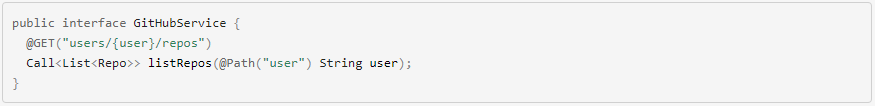
\includegraphics[keepaspectratio, width=12cm]{gambar/retrofit1}
		\caption{Contoh \textit{retrofit} mengubah API menjadi \textit{interface} \citep{retrofit2023}}
		\label{gambar:gambar_49}
	\end{figure}
	
	\item Kelas \textit{Retrofit} menghasilkan implementasi \textit{interface GitHubService}.
	\begin{figure}[H]
		\centering
		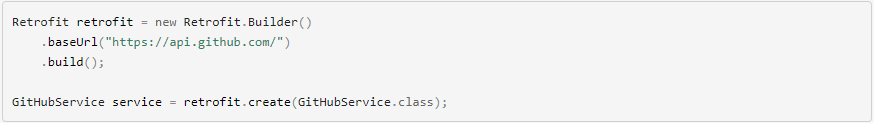
\includegraphics[keepaspectratio, width=12cm]{gambar/retrofit2}
		\caption{Kelas \textit{retrofit} \citep{retrofit2023}}
		\label{gambar:gambar_50}
	\end{figure}
	
	\item Setiap \textit{Call} dari \textit{GitHubService} yang dibuat dapat membuat \textit{request} HTTP sinkron atau asinkron ke server web jarak jauh.
	\begin{figure}[H]
		\centering
		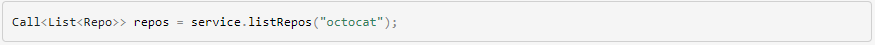
\includegraphics[keepaspectratio, width=12cm]{gambar/retrofit3}
		\caption{\textit{Call} \citep{retrofit2023}}
		\label{gambar:gambar_51}
	\end{figure}
	\end{enumerate}

Menggunakan anotasi untuk menjelaskan request HTTP:
	\begin{enumerate}
		\item Penggantian parameter URL dan dukungan parameter kueri
		\item Konversi objek ke request body (misalnya JSON, protocol buffers)
		\item Multi-bagian request body dan unggahan file
	\end{enumerate}
	
\item Deklarasi API

Anotasi pada metode interface dan parameternya menunjukkan bagaimana request akan ditangani.
	\begin{enumerate}
	\item \emph{Request method}
	
	Setiap metode harus memiliki anotasi HTTP yang menyediakan metode request dan URL relatif. Ada delapan anotasi bawaan: HTTP, GET, POST, PUT, PATCH, DELETE, OPTIONS, dan HEAD. URL relatif resource ditentukan dalam anotasi.
	\begin{figure}[H]
		\centering
		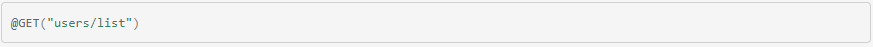
\includegraphics[keepaspectratio, width=12cm]{gambar/retrofit4}
		\caption{Contoh request GET \citep{retrofit2023}}
		\label{gambar:gambar_52}
	\end{figure}
	
	Dapat juga menentukan parameter kueri di URL
	\begin{figure}[H]
		\centering
		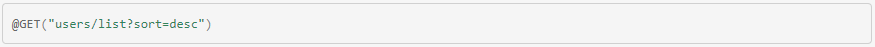
\includegraphics[keepaspectratio, width=12cm]{gambar/retrofit5}
		\caption{Contoh request GET dengan menentukan parameter kueri di URL \citep{retrofit2023}}
		\label{gambar:gambar_53}
	\end{figure}
	
	\item Manipulasi URL
	
	Request URL dapat diperbarui secara dinamis menggunakan blok dan parameter pengganti pada metode. Blok pengganti adalah string alfanumerik yang dikelilingi oleh { dan }. Parameter yang sesuai harus dianotasi dengan @Path menggunakan string yang sama.
	\begin{figure}[H]
		\centering
		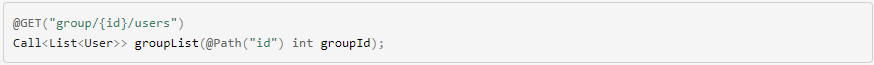
\includegraphics[keepaspectratio, width=12cm]{gambar/retrofit6}
		\caption{Contoh request URL secara dinamis \citep{retrofit2023}}
		\label{gambar:gambar_54}
	\end{figure}
	
	Parameter kueri juga dapat ditambahkan.
	\begin{figure}[H]
		\centering
		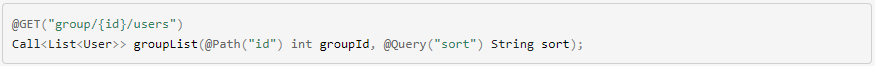
\includegraphics[keepaspectratio, width=12cm]{gambar/retrofit7}
		\caption{Contoh parameter kueri ditambahkan \citep{retrofit2023}}
		\label{gambar:gambar_55}
	\end{figure}
	
	Untuk kombinasi parameter kueri yang kompleks, Map dapat digunakan.
	\begin{figure}[H]
		\centering
		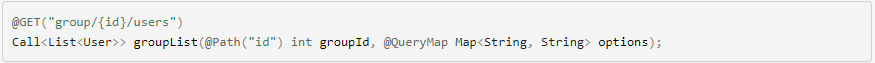
\includegraphics[keepaspectratio, width=12cm]{gambar/retrofit8}
		\caption{Contoh menggunakan Map \citep{retrofit2023}}
		\label{gambar:gambar_56}
	\end{figure}
	
	\item \emph{Request Body}
	
	Sebuah objek dapat ditentukan untuk digunakan sebagai body request HTTP dengan anotasi @Body.
	\begin{figure}[H]
		\centering
		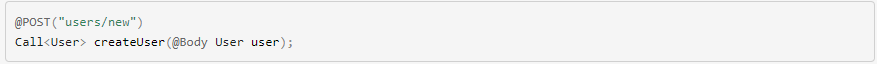
\includegraphics[keepaspectratio, width=12cm]{gambar/retrofit9}
		\caption{Contoh anotasi Body \citep{retrofit2023}}
		\label{gambar:gambar_57}
	\end{figure}
	
	Objek juga akan dikonversi menggunakan konverter yang ditentukan pada instance Retrofit. Jika tidak ada konverter yang ditambahkan, hanya RequestBody yang dapat digunakan.
	
	\item Formulir dikode dan multipart
	
	Metode juga dapat dideklarasikan untuk mengirim data yang disandikan bentuk dan multibagian. Data yang disandikan formulir dikirim ketika @FormUrlEncoded ada di metode. Setiap pasangan nilai kunci dianotasi dengan @Field yang berisi nama dan objek yang memberikan nilai.
	\begin{figure}[H]
		\centering
		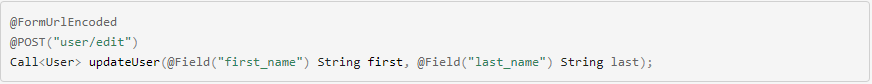
\includegraphics[keepaspectratio, width=12cm]{gambar/retrofit10}
		\caption{Contoh dikode \citep{retrofit2023}}
		\label{gambar:gambar_58}
	\end{figure}
	
	Request multipart digunakan ketika @Multipart hadir pada metode. Bagian dideklarasikan menggunakan anotasi @Part.
	\begin{figure}[H]
		\centering
		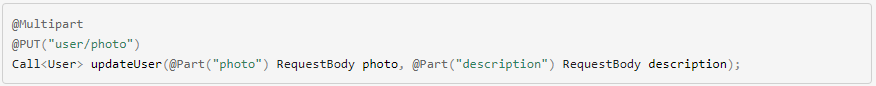
\includegraphics[keepaspectratio, width=12cm]{gambar/retrofit11}
		\caption{Contoh multipart \citep{retrofit2023}}
		\label{gambar:gambar_59}
	\end{figure}
	
	Bagian multipart menggunaakn salah satu konverter Retrofit atau mereka dapat mengimplementasikan RequestBody untuk menangani serialisasi mereka sendiri.
	
	\item Manipulasi \emph{header}
	
	Kita dapat mengatur tajuk statis untuk suatu metode menggunakan anotasi @Headers.
	\begin{figure}[H]
		\centering
		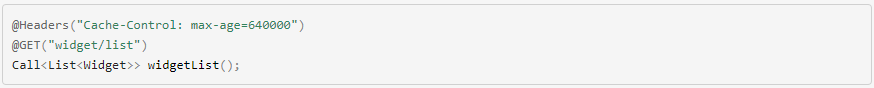
\includegraphics[keepaspectratio, width=12cm]{gambar/retrofit12}
		\caption{Contoh anotasi header \citep{retrofit2023}}
		\label{gambar:gambar_60}
	\end{figure}
	
	\begin{figure}[H]
		\centering
		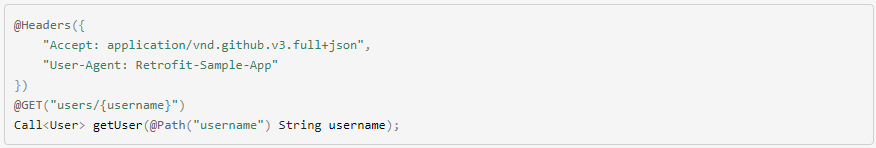
\includegraphics[keepaspectratio, width=12cm]{gambar/retrofit13}
		\caption{Contoh anotasi header \citep{retrofit2023}}
		\label{gambar:gambar_61}
	\end{figure}
	
	Perhatikan bahwa header tidak saling menimpa. Semua header dengan nama yang sama akan disertakan dalam request.
	Requset header dapat diperbarui secara dinamis menggunakan anotasi @Header. Parameter yang sesuai harus diberikan ke @Header. Jika nilainya null, header akan dihilangkan. Jika tidak, toString akan dipanggil pada nilai, dan hasilnya digunakan.
	\begin{figure}[H]
		\centering
		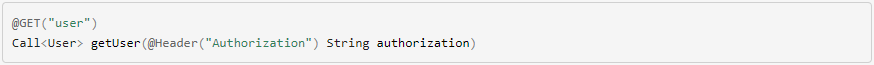
\includegraphics[keepaspectratio, width=12cm]{gambar/retrofit14}
		\caption{Contoh header dinamis \citep{retrofit2023}}
		\label{gambar:gambar_62}
	\end{figure}
	
	Mirip dengan parameter kueri, untuk kombinasi tajuk yang kompleks, Map dapat digunakan.
	\begin{figure}[H]
		\centering
		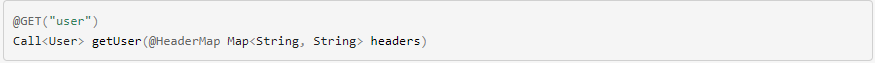
\includegraphics[keepaspectratio, width=12cm]{gambar/retrofit15}
		\caption{Contoh header kompleks menggunakan Map \citep{retrofit2023}}
		\label{gambar:gambar_63}
	\end{figure}
	
	Header yang perlu ditambahkan ke setiap request dapat ditentukan menggunakan interseptor OkHttp.
	\end{enumerate}
	
\item Konfigurasi retrofit

Retrofit adalah kelas yang digunakan untuk mengubah interface API menjadi objek yang dapat dipanggil. Secara default, Retrofit akan memberi standar yang normal untuk platform tetapi memungkinkan untuk penyesuaian.

	\begin{enumerate}
	\item Converters
	
	Secara default, Retrofit hanya dapat melakukan deserialize body HTTP ke dalam tipe ResponseBody OkHttp dan hanya dapat meneripa tipe RequestBody untuk @Body. Konverter dapat ditambahkan untuk mendukung jenis lain. Enam modul bersaudara mengadaptasi pustaka serialisasi populer untuk kenyamanan pengguna.
		\begin{enumerate}
		\item Gson: com.squareup.retrofit2:converter-gson
		\item Jackson: com.squareup.retrofit2:converter-jackson
		\item Moshi: com.squareup.retrofit2:converter-moshi
		\item Protobuf: com.squareup.retrofit2:converter-protobuf
		\item Wire: com.squareup.retrofit2:converter-wire
		\item Simple XML: com.squareup.retrofit2:converter-simplexml
		\item JAXB: com.squareup.retrofit2:converter-jaxb
		\item Scalars (primitives, boxed, dan String): com.squareup.retrofit2:converter-scalars
		\end{enumerate}
		
	Berikut adalah contoh penggunaan kelas GsonConverterFactory untuk menghasilkan implementasi interface GitHubService yang menggunakan Gson untuk deserialisasinya.
	\begin{figure}[H]
		\centering
		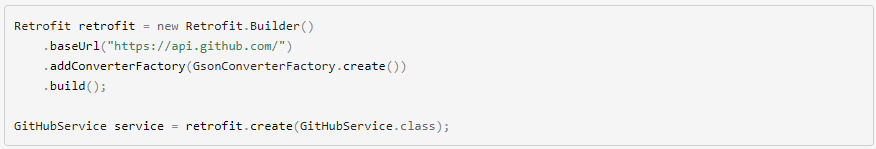
\includegraphics[keepaspectratio, width=12cm]{gambar/retrofit16}
		\caption{Contoh kelas GsonConverterFactory \citep{developerandroid}}
		\label{gambar:gambar_64}
	\end{figure}
	
	\item Custom Converters
	
	Jika perlu berkomunikasi dengan API yang menggunakan format konten yang tidak didukung Retrofit secara langsung (misalnya YAML, txt, format kustom) atau ingin menggunakan pustakan lain untuk mengimplementasikan format yang sudah ada, pengguna dapat dengan mudah membuat konverter pengguna sendiri. Buat kelas yang memperluas kelas Converter.Factory dan berikan instance saat membuat adaptor pengguna.
	\end{enumerate}

\item Download retrofit

Kode sumber Retrofit, sampelnya, dan situs web resmi tersedia di GitHub. Lalu pada Gradle tambahkan:
\begin{figure}[H]
	\centering
	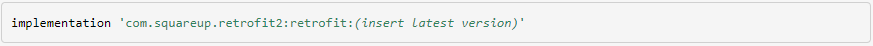
\includegraphics[keepaspectratio, width=12cm]{gambar/retrofit17}
	\caption{Contoh mendownload retrofit pada Gradle \citep{developerandroid}}
	\label{gambar:gambar_65}
\end{figure}

Retrofit membutuhkan minimal Java 8+ atau Android API 21+.
\end{enumerate}

\section{Manajemen Keperawatan}
\begin{enumerate}
\item \textit{Medical Record}

Sebelum dilakukannya proses penyembuhan oleh perawat, pasien diharuskan untuk mengisi data-data terkait diri mereka. Data-data tersebut diperlukan dalam meningkatkan keberhasilan penyembuhan sang pasien. Salah satu data yang diperlukan dalam proses penyembuhan yaitu rekap kunjungan pasien.

\item Rekap kunjungan pasien

Hal ini untuk mencatat tanggal kunjungan, jumlah kunjungan, perawat yang mengobati, dan hasil dari pemeriksaan serta keterangan yang diperlukan untuk membantu proses penyembuhan di hari kunjungan berikutnya.

\item Surat pernyataan persetujuan tindakan

Selanjutnya yaitu surat pernyataan persetujuan dari pasien. Pihak rumah sakit atau klinik meminta agar pasien menandatangani surat pernyataan persetujuan tindakan ini untuk dapat leluasa dalam melakukan perawatan. Pasien diberikan informasi mengenai kondisi pasien tersebut dan diharap mengerti serta memahami konsekuensi dari tindakan yang akan dilakukan sesuai dengan penjelasan yang telah diberikan oleh tenaga kesehatan yang melakukan perawatan.

\item Status pasien

Status pasien ini berisi data-data pribadi pasien tersebut. Status pasien terdiri dari nomor registrasi, nama lengkap pasien, agama/keyakinan pasien, tempat, tanggal lahir dan usia pasien, jenis kelamin pasien, alamat dan nomor telepon rumah pasien, nomor \textit{handphone} dan alamat email pasien, diagnosa keperawatan saat ini, \textit{therapist} utama, tim \textit{therapist}, dan alergi yang dialami oleh pasien.

\item Pengkajian umum luka

Pada pengkajian umum luka ini meliputi riwayat kejadian luka, riwayat perawatan sebelumnya dan faktor-faktor penyulit proses penyembuhan luka pada pasien.

\item Pengkajian lokal luka

Perawat melakukan pemeriksaan pada pasien yang nantinya akan menjadi penunjang keberhasilan penyembuhan luka pasien. Pemeriksaan yang dilakukan oleh perawat ialah tipe luka, tipe penyembuhan, gambar luka, pemeriksaan tanda-tanda vital dan penunjang, serta pemeriksaan fisik dan penunjang lainnya.
Dilanjutkan dengan skoring luka yang dilakukan oleh perawat menggunakan assessment tools yang sudah disiapkan. Dalam gambar ini saya mengambil contoh skoring luka berdasarkan klinik moist care pusat penyembuhan luka.

\item Catatan perkembangan

Diakhir pemeriksaan pengkajian luka, perawat atau therapist memberi kesimpulan tujuan keperawatan yang nantinya dijadikan evaluasi dan rencana tindakan atau intervensi selanjutnya pada pasien.

\item Standar kompetensi perawat dalam perawatan luka

\textit{Enterostomal Therapy Nurse} atau ETN merupakan spesialisasi keperawatan dalam bidang \textit{enterostomal therapy}, \textit{“expert”} dalam melakukan asuhan keperawatan \textit{stoma}, perawatan luka dan \textit{inkontinensia}. Atau yang dikenal dengan nama lainnya adalah \textit{Wound Stoma and Continence Nurse Specialist} atau WOCNS. Pertama kalinya \textit{“Enterostomal Therapist”} dikenalkan oleh Dr. Rupert Turnbull, dari \textit{Cleveland clinic}, USA pada tahun 1958. Beliau bersama dengan salah satu pasien ileostominya, Mrs. Norma Gill, mengadakan program pelatihan untuk para profesional pertama kali tentang bagaimana membantu pasien stoma dalam menjalani kehidupannya yang baru.

Sejak pelatihan pertama di \textit{Cleveland clinic}, USA, tanggung jawab keilmuan \textit{Enterostomal Therapist} semakin berkembang, kemudian berdirilah sekolah perawatan \textit{Enterostomal Therapist} dibawah \textit{World Council of Enterostomal Therapist}(WCET) atau yang dikenal dengan ETNEP(\textit{Enterostomal Therapy Nurse Education Programme}).
Di akhir tahun 1970, \textit{Enterostomal Therapist} mengembangkan diri pada bidang spesialisasi managemen perawatan luka kronik. Awalnya adalah karena keberhasilan dalam merawat komplikasi kulit disekitar stoma. Saat ini, hampir sebagian team \textit{Enterostomal Therapist} melakukan perawatan luka kronik yang meliputi \textit{pressure ulcer}, \textit{dehisensi} luka operasi, \textit{fistula}, \textit{malignant wound}, \textit{vascular ulcer} dan luka diabetikum.

ETN dalam wadah WCET (\textit{World Council of Enterostomal Therapists}) sebagai lembaga non profit internasional telah mengembangkan sayapnya diseluruh penjuru eropa, america dan asia pasific. Keberadaan organisasi ini telah diakui secara international sebagai profesi keperawatan yang profesional. Pengembangan profesi dilakukan dengan mengadakan kongres 2 tahunan dan ETNEP. Di lima tahun terakhir ini, WCET telah membuka diri dengan konsep \textit{twinning} program edukasi untuk lebih memperluas bidang keilmuan \textit{enterostomal therapy nurse} terutama di asia, untuk mempermudah adanya kesulitan dalam bahasa.

Peran ETN adalah untuk memberikan perawatan secara langsung dan konseling pada ostomate selama berada di RS dan di rumah. Memfasilitasi rehabilitasi bagi ostomate untuk berhubungan dengan dokter, ahli gizi atau \textit{sosial worker}. Merancang program edukasi bagi ostomate dan keluarganya dalam bentuk grup/ kelompok. Berpartisipasi dalam pendidikan keperawatan dalam hal pembelajaran tentang perawatan ostomi, \textit{wound} dan \textit{inkontinensia} Melakukan uji coba produk dan melakukan penelitian yang berhubungan dengan pemakaiannya untuk meningkatkan kualitas pelayanan. Melakukan pencatatan data, statistik dan yang berhubungan dengan pelayanan \textit{Enterostomal Therapy}.

Di Indonesia, organisasi yang resmi menyelenggarakan pendidikan ETNEP dari WCET adalah InWOCNA (\textit{Indonesia Wound Ostomy Continence Nurse Association}). Dengan mengikuti ETNEP, perawat dapat sertifikat keahlian resmi dari InWOCNA dan sudah diakui oleh PPNI (Persatuan Perawat Nasional Indonesia) bahwa perawat tersebut telah mengikuti pelatihan sesuai dengan kurikulum InWOCNA. \citep{inwocna}

\end{enumerate}
\begin{figure}[H]
	\centering
	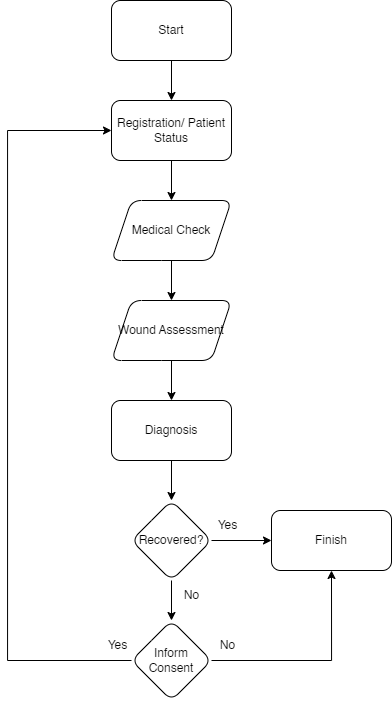
\includegraphics[keepaspectratio, width=8cm]{gambar/flowchart_manajemen_perawatan_luka}
	\caption{Flowchart manajemen keperawatan}
	\label{gambar:gambar_73}
\end{figure}

\section{\emph{Scrum}}

Dalam mengerjakan penelitian ini saya menggunakan scrum untuk dijadikan kerangka kerja agar dapat menghasilkan solusi yang adaptif untuk masalah yang kompleks. Mengenai metode scrum ini sudah dijelaskan dengan sangat lengkap di penelitian sebelumnya oleh Salsa Rahmadati yang berjudul “Perancangan Aplikasi Pengkajian Luka Kronis Berbasis Android Modul Pengolahan Citra”.
%!TEX root = ./template-skripsi.tex
%-------------------------------------------------------------------------------
%                            BAB III
%               			PEMBAHASAN
%-------------------------------------------------------------------------------

\chapter{METODOLOGI PENELITIAN}

\section{Deskripsi Sistem}

Penelitian yang akan dibuat oleh penulis adalah memperbaharui dan melanjutkan penelitian sistem aplikasi yang telah dibuat sebelumnya oleh (Rahmadati, 2023) yang berjudul “PERANCANGAN APLIKASI PENGKAJIAN LUKA KRONIS BERBASIS ANDROID MODUL PENGOLAHAN CITRA” dalam pembuatan aplikasi skoring luka. Aplikasi ini berfungsi sebagai alat untuk membantu perawat dalam mengidentifikasi tingkat penyembuhan luka pasien. Selain hal tersebut, aplikasi ini juga akan diintegrasi dengan sistem pewarnaan luka otomatis (Aprillia, 2021) dan sistem anotasi luka otomatis (Rizki, 2022) serta menambahkan fitur manajemen keperawatan. Penelitian ini juga akan terhubung dengan (Insan, 2023) pada database yang sedang dikembangkan.

Penelitian ini dimulai dengan menganalisis kebutuhan, kemudian lanjut ke proses pengembangan, dan diakhiri dengan pengujian serta evaluasi. Tahapan penelitian yang penulis lakukan dalam penelitian aplikasi ini dapat dilihat pada gambar 3.1.


\begin{figure}[H]
	\centering
	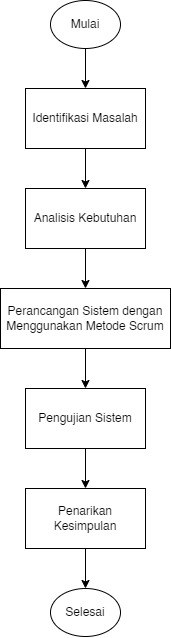
\includegraphics[keepaspectratio, width=4cm]{gambar/tahapan_penelitian}
	\caption{Tahapan Penelitian}
	\label{gambar:tahapan_penelitian}
\end{figure}

\section{Analisa Kebutuhan}

Berdasarkan wawancara dengan bu Ratna pada lampiran A, prioritas fitur pada aplikasi ini terfokus pada kajian luka yang belum ada pada aplikasi sebelumnya (Rahmadati, 2022) yang terdapat pada \textit{Bates-Jensen Wound Assessment Tools} dan fitur manajemen keperawatan serta penambahan user pada pasien. Berikut adalah \textit{usecase} yang telah didefinisikan berdasarkan wawancara.

\begin{figure}[H]
	\centering
	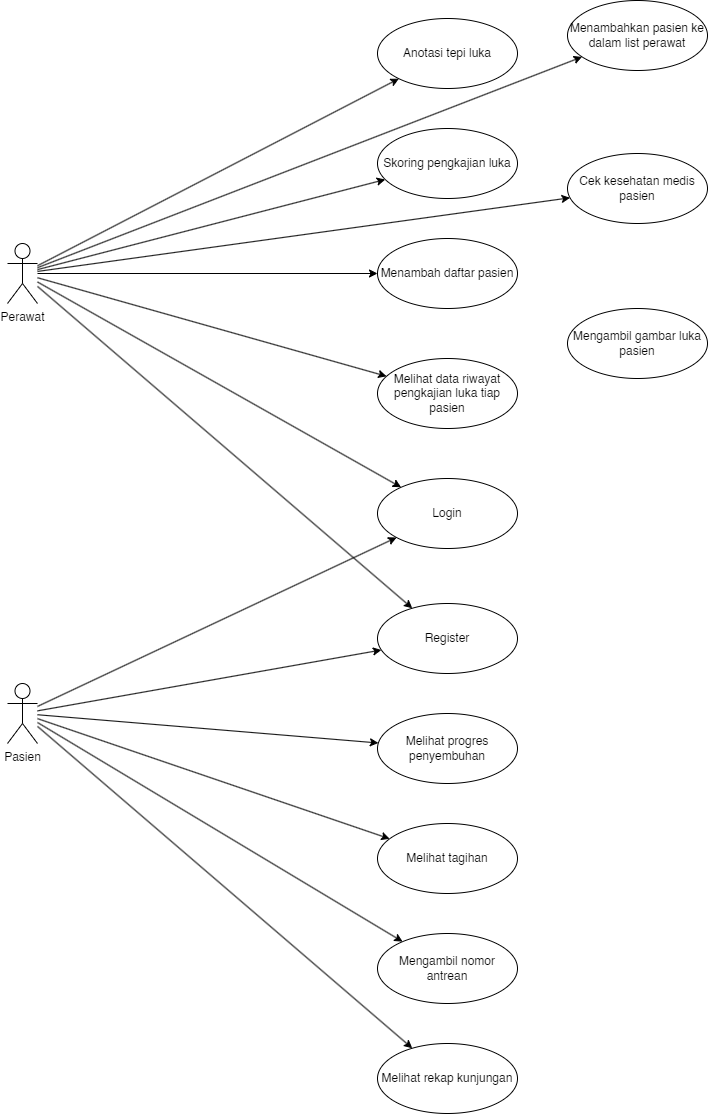
\includegraphics[keepaspectratio, width=8cm]{gambar/usecase}
	\caption{Use Case}
	\label{gambar:use_case}
\end{figure}

Perangkat yang dibutuhkan oleh penulis adalah sebagai berikut:
\begin{enumerate}
\item Laptop dengan spesifikasi minimum dapat menjalankan program aplikasi android studio.
\item Smartphone android untuk uji coba aplikasi ketika selesai.
\item Android Studio sebagai IDE untuk pembuatan aplikasi berbasis Android.
\item Kotlin sebagai bahasa pemrograman penyusun aplikasi.
\item Flask sebagai web framework.
\item MongoDB sebagai basis data.
\item Figma untuk desain tampilan aplikasi.
\end{enumerate}

\section{Perancangan Sistem}

Metode perancangan sistem pada penelitian ini sesuai dengan komponen yang ada di dalam metode \textit{Scrum}. Komponen-komponen tersebut terdiri dari \textit{product backlog, sprint backlog, sprint, daily scrum,} dan pengujian sistem. Tahapan ini dilakukan setelah dilakukannya tahapan analisis kebutuhan.

\begin{figure}[H]
	\centering
	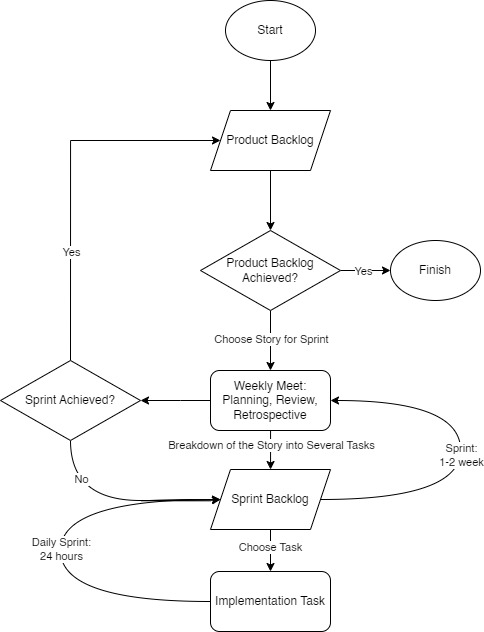
\includegraphics[keepaspectratio, width=10cm]{gambar/metode_scrum}
	\caption{Tahapan Pengembangan Metode Scrum}
	\label{gambar:scrum}
\end{figure}

\begin{enumerate}
\item \textit{Product Backlog}

Product Backlog berisi fitur-fitur yang dibuat berdasarkan kebutuhan pengguna dan sudah didiskusikan dengan Scrum Master. Tabel 3.1 merupakan rincian product backlog dari aplikasi yang akan dibuat.

\begin{table}[H]
	\caption{\textit{Product Backlog}}
	\label{product_backlog}
	\begin{tabular}{@{} |p{0.5cm}|p{7cm}|p{1.5cm}|p{2cm}|p{2cm}| @{}}
		\hline
		\textbf{No} & \textbf{\textit{User Story}} & \textbf{\textit{Role}} & \textbf{\textit{Priority}} & \textbf{\textit{Sprint}} \\
		\hline
		1 & \textit{Skoring Bates-Jensen} & Perawat & High & \multirow{5}{2cm}{1} \\
		\cline{1-4}
		2 & Konversi seluruh activity menjadi fragment & & High &  \\
		\cline{1-4}
		3 & Login user & Perawat, Pasien & High &  \\
		\hline
		4 & Evaluasi kondisi kesehatan pasien sebelum perawatan & Perawat & High & 2 \\
		\hline
		5 & Catatan perkembangan/ diagnosis untuk langkah penyembuhan selanjutnya & Perawat & High & 3 \\
		\hline
		6 & Rekap kunjungan pasien & Perawat & High & 4 \\
		\hline
		7 & Implementasi web service program warna luka & Perawat & Low & \multirow{4}{2cm}{5} \\
		\cline{1-4}
		8 & Implementasi web service anotasi luka & Perawat & Low &  \\
		\cline{1-4}
		9 & Mengembangkan progres penyembuhan luka pasien penelitian sebelumnya & Perawat & Low &  \\
		\hline
		10 & \textit{Wound History} & Perawat & High & 6 \\
		\hline
		11 & Registrasi akun pasien & Pasien & Low & \multirow{4}{2cm}{7} \\
		\cline{1-4}
		12 & Mengambil nomor antrean & Pasien & Low &  \\
		\cline{1-4}
		13 & Melihat rekap kunjungan & Pasien & Low &  \\
		\cline{1-4}
		14 & Melihat histori kajian & Pasien & High &  \\
		\hline
		15 & Inventaris & Perawat & Low & 8 \\
		\hline
		16 & Menambah pasien ke dalam akun perawat & Perawat & Low & 9 \\
		\hline
	\end{tabular}
\end{table}
Berdasarkan tabel di atas, Product Backlog pada penelitian ini terdiri dari 5 komponen yaitu: User Story, Role, Sprint, Status. User Story berisi fitur-fitur besar yang akan dibuat pada aplikasi ini. Komponen role pada tabel ini menandakan siapa yang menggunakan fitur tersebut. Priority menentukan tingkat prioritas dari sebuah User Story. Sprint menandakan informasi urutan fitur yang akan dibuat. Dan status menjelaskan apakah fitur tersebut sudah selesai atau belum.

\item Sprint Backlog

Sprint Backlog adalah daftar task yang perlu dikerjakan ataupun yang sudah dikerjakan pada sprint. Di dalam sprint backlog, berbagai task kecil dibuat. Dengan sprint backlog, seluruh anggota tim dapat melihat perkembangan dari setiap pekerjaan.

\item Sprint

Setelah dilakukan perencanaan pada Sprint Backlog, maka pengerjaan sprint sudah dapat dimulai dan harus mengikuti jadwal pengerjaan yang telah disepakati bersama tim. Dalam penelitian ini, interval sprint yang digunakan adalah satu sampai dua minggu. Berikut merupakan laporan hasil Sprint-1.
	
	
\item Sprint Review dan Sprint Retrospective
	
Sprint review dan sprint retrospective dilakukan pada setiap wal pekan yaitu di hari Selasa melalui daring menggunakan platform discord dan tatap muka secara langsung di UNJ. Pada awal pekan ini akan dilakukan evaluasi mengenai perkembangan proses pembuatan aplikasi maupun hambayan yang terjadi selama pengerjaan di setiap sprint.
	
\item Deploy
	
Pada tahap ini peneliti akan melakukan uji aplikasi pengkajuan luka kronis menggunakan dua jenis pengujian yaitu unit testing dan user acceptance test (UAT). Pengujian unit testing dilaksanakan oleh tim internal developer untuk memastikan fungsi-fungsi pada aplikasi yang telah dikembangkan dapat berjalan dengan baik. Sedangkan UAT dilaksanakan oleh pengguna yang mengetahui apakah aplikasi sudah sesuai kebutuhan dan layak untuk diuji secara masif.
\end{enumerate}

\section{Pengujian}

Pada tahap ini peneliti akan melakukan uji aplikasi pengkajuan luka kronis menggunakan dua jenis pengujian yaitu unit testing dan user acceptance test (UAT). Pengujian unit testing dilaksanakan oleh tim internal developer untuk memastikan fungsi-fungsi pada aplikasi yang telah dikembangkan dapat berjalan dengan baik. Sedangkan UAT dilaksanakan oleh pengguna yang mengetahui apakah aplikasi sudah sesuai kebutuhan dan layak untuk diuji secara masif.

\begin{enumerate}
\item Unit Testing

Skenario pada unit testing dibuat berdasarkan product backlog. Adapun skenario dari unit testing yang akan dilaksanakan terdapat pada tabel 3.3.
	
	\begin{longtable}[c]{@{} |p{4cm}|p{9.3cm}| @{}}
 	\caption{Skenario \textit{Unit Testing} \label{unit_testing}}\\

 	\hline
 	\multicolumn{2}{| c |}{\textbf{Skenario \textit{Unit Testing}}}\\
 	\hline
 	\centering{\textbf{Uji Fitur}} & \centering{\textbf{Skenario Pengujian}}  
 	\endfirsthead

 	\hline
 	\multicolumn{2}{| c |}{\textbf{Skenario \textit{Unit Testing}}}\\
 	\hline
 	\centering{\textbf{Uji Fitur}} & \centering{\textbf{Skenario Pengujian}}
 	\endhead

 	\hline
 	\endfoot

 	\hline
 	\endlastfoot

 	\hline
 	
 	Halaman Awal & Saat aplikasi dibuka akan muncul tampilan awal dengan pilihan "Login" dan "Register"\\
	\hline
	& Jika tombol "Login" ditekan, guest akan masuk ke halaman Login\\
	\hline
	& Jika tombol "Register" ditekan, guest akan masuk ke halaman Register\\
	\hline
	Register & Ketika mengisi form registrasi dengan lengkap kemudian submit, maka akan kembali ke halaman Login\\
	\hline
	& Ketika mengisi form registrasi tidak lengkap kemudian submit, maka akan menampilkan pesan kesalahan untuk melengkapi data yang kosong\\
	\hline
	Login & Ketika mengisi form login dengan data yang tidak sesuai kemudian klik submit, maka akan menampilkan pesan kesalahan username atau password\\
	\hline
	& Ketika mengisi form login dengan data yang sesuai dengan role perawat, maka akan masuk ke halaman beranda perawat\\
	\hline
	& Ketika mengisi form login dengan data yang sesuai dengan role pasien, maka akan masuk ke halaman beranda pasien\\
	\hline
	Beranda Perawat & Saat ikon profil pada kanan atas di-klik maka akan muncul halaman profil perawat\\
	\hline
	& Saat tombol daftar pasien di-klik maka akan muncul halaman daftar pasien\\
	\hline
	& Saat tombol pewarnaan luka ditekan, maka akan muncul halaman pewarnaan luka otomatis\\
	\hline
	& Saat tombol medical record ditekan, maka akan muncul halaman medical record pasien\\
	\hline
	Tambah hasil kajian & Saat pertama kali klik tombol tambah kajian baru muncul halaman pemeriksaan kesehatan pasien sebelum perawatan\\
	\hline
	& Ketika mengisi form pemeriksaan kesehatan dengan tidak lengkap maka akan menampilkan pesan kesalahan bahwa data yang diisi kurang sesuai atau belum lengkap\\
	\hline
	& Ketika mengisi form pemeriksaan kesehatan dengan lengkap maka akan masuk ke halaman ambil foto luka\\
	\hline
	& Ketika pengguna menekan tombol kamera, maka akan masuk ke halaman pengambilan foto luka\\
	\hline
	& Ketika pengguna selesai mengambil foto luka, maka akan diarahkan ke halaman anotasi tepi luka otomatis.\\
	\hline
	& Ketika anotasi tepi luka otomatis selesai bekerja, maka pengguna dapat menekan tombol "SAVE" untuk lanjut ke halaman kajian luka atau tekan tombol "EDIT" untuk menganotasi luka secara manual.\\
	\hline
	& Ketika mengisi form kajian luka secara tidak lengkap kemudian klik "NEXT", maka akan muncul pesan kesalahan bahwa data yang diisi belum lengkap\\
	\hline
	& Ketika mengisi form kajian luka secara lengkap kemudian klik "NEXT", maka akan diarahkan ke halaman tujuan perawatan.\\
	\hline
	& Ketika mengisi form tujuan perawatan secara tidak lengkap kemudian klik submit, maka akan muncul pesan kesalahan bahwa data yang diisi belum lengkap\\
	\hline
	& Ketika mengisi form tujuan perawatan secara lengkap kemudian klik submit, maka akan diarahkan ke halaman detail pasien yang baru saja diinput\\
	\hline
	Detail pasien & Saat masuk pertama kali ke halaman detail pasien, maka akan muncul informasi umum pasien dan progres tingkat kesembuhan luka pasien berdasarkan skoring kajian luka sebelumnya\\
	\hline
	& Saat tab Histori Kajian diklik maka akan muncul histori kajian pasien dan progres tingkat kesembuhan luka pasien berdasarkan skoring kajian luka sebelumnya\\
	\hline
	Beranda Pasien & Saat ikon profil pada kanan atas di-klik maka akan muncul halaman profil pasien\\
	\hline
	& Saat tombol riwayat kajian luka ditekan, maka akan muncul halaman riwayat kajian luka pasien\\
	\hline
	& Saat tombol rekap kunjungan ditekan, maka akan muncul halaman rekap kunjungan pasien\\
	\hline
	& Saat tombol medical record ditekan, maka akan muncul halaman medical record pasien\\
	\hline
	Profil Pasien & Saat ikon profil pada kanan atas di-klik maka akan muncul halaman profil pasien\\
	\hline
	& Saat tombol ambil antrean ditekan, maka akan diarahkan ke halaman antrean.\\
	\hline
	& Saat tombol riwayat kajian luka ditekan, maka akan muncul halaman riwayat kajian luka pasien.\\
	\hline
	& Saat tombol rekap kunjungan ditekan, maka akan muncul halaman rekap kunjungan pasien.\\
	\hline
	& Saat tombol medical record ditekan, maka akan muncul halaman medical record pasien.\\
	\hline
	Antrean & Saat masuk pertama kali ke halaman antrean, maka akan muncul nomor antrean saat ini, nama, nomor registrasi dan tombol ambil antrean.\\
	\hline
	& Saat tombol antrean ditekan, maka akan muncul nomor antrean yang diambil lalu tombol ambil antrean berubah menjadi selesai berobat.\\
	\hline
	& Saat tombol selesai berobat ditekan maka tombol tersebut akan menghilang lalu diarahkan kembali ke halaman beranda.\\
	\hline
	Riwayat kajian luka & Saat ikon profil pada kanan atas di-klik maka akan muncul halaman profil pasien\\
	\hline
	& Saat tombol riwayat kajian luka ditekan, maka akan muncul halaman riwayat kajian luka pasien\\
	\hline
	& Saat tombol rekap kunjungan ditekan, maka akan muncul halaman rekap kunjungan pasien\\
	\hline
	& Saat tombol medical record ditekan, maka akan muncul halaman medical record pasien\\
	\hline
	Rekap kunjungan & Saat ikon profil pada kanan atas di-klik maka akan muncul halaman profil pasien\\
	\hline
	& Saat tombol riwayat kajian luka ditekan, maka akan muncul halaman riwayat kajian luka pasien\\
	\hline
	& Saat tombol rekap kunjungan ditekan, maka akan muncul halaman rekap kunjungan pasien\\
	\hline
	& Saat tombol medical record ditekan, maka akan muncul halaman medical record pasien\\
	\hline
 	\end{longtable}
 	
\item User Acceptance Testing

Skenario dalam Uji Penerimaan Pengguna disusun berdasarkan fitur-fitur yang dapat diakses oleh pengguna dalam backlog produk. Detail skenario UAT yang akan dilaksanakan tercantum dalam tabel 3.4.

\begin{longtable}[c]{@{} |p{4cm}|p{7cm}|p{2.3cm}| @{}}
 	\caption{Skenario \textit{Unit Acceptance Testing} \label{unit_acceptance_testing}}\\

 	\hline
 	\centering{\textbf{Uji Fitur}} & \centering{\textbf{Skenario Pengujian}} & \centering{\textbf{Jenis Pengujian}}
 	\endfirsthead

 	\hline
 	\centering{\textbf{Uji Fitur}} & \centering{\textbf{Skenario Pengujian}} & \centering{\textbf{Jenis Pengujian}}
 	\endhead

 	\hline
 	\endfoot

 	\hline
 	\endlastfoot

 	\hline
 	
 	Registrasi & Menekan tombol buat akun lalu mengisi 
form registrasi kemudian submit & UAT\\
	\hline
	Login & Menekan tombol login lalu mengisi form login dengan NIP dan password kemudian submit & UAT\\
	\hline
	Daftar pasien & Klik tombol daftar pasien pada beranda kemudian menampilkan daftar pasien & UAT\\
	\hline
	Melihat detail pasien & Klik tombol daftar pasien pada beranda kemudian klik pasien yang ingin dilihat detailnya & UAT\\
	\hline
	Galeri luka & Klik tombol galeri luka kronis pada beranda & UAT\\
	\hline
	Arsir warna luka & Klik tombol arsir warna luka kronis pada beranda kemudian unggah gambar melalui galeri lalu mengarsir warna luka dan submit & UAT\\
	\hline
	Menambahkan kajian luka baru & Buka halaman detail pasien lalu klik tab histori kajian luka kemudian klik tombol tambah hasil kajian dilanjutkan dengan isi form kajian dan submit & UAT\\
	\hline
	Anotasi tepi luka & Buka halaman detail pasien lalu klik tab histori kajian luka kemudian klik icon tambah dilanjutkan dengan memfoto luka kronis lalu melakukan anotasi tepi luka dan submit & UAT\\
	\hline
	Anotasi diameter luka & Setelah melakukan anotasi tepi luka, masuk ke halaman anotasi diameter luka kemudian melakukan anotasi diameter luka dan submit & UAT\\
	\hline
	Melihat histori kajian luka & Buka halaman detail pasien lalu klik tab histori kajian luka & UAT\\
	\hline
	Melihat detail dari histori kajian luka & Buka halaman detail pasien lalu klik tab histori kajian luka kemudian klik card sesuai dengan tanggal kajian luka yang ingin dilihat & UAT\\
	\hline
	Galeri luka satu pasien & Buka halaman detail pasien lalu klik tab galeri luka pasien & UAT\\
	\hline
	Profil perawat & Dari halaman beranda, klik ikon profil pada kanan atas & UAT\\
	\hline
	Logout & Pada halaman profil perawat, klik tombol logout & UAT\\
	\hline
 	\end{longtable}
\end{enumerate}


%\subsection{\textit{Daily Scrum}}

%Pada akhir pekan di akhir setiap \textit{sprint}, akan diadakan \textit{voice call} untuk membahas perkembangan dan hambatan pada setiap \textit{sprint}.
%!TEX root = ./template-skripsi.tex
%-------------------------------------------------------------------------------
%                            	BAB IV
%               		KESIMPULAN DAN SARAN
%-------------------------------------------------------------------------------

\chapter{HASIL DAN PEMBAHASAN}

\section{Pembahasan}
Perancangan aplikasi pengkajian luka kronis ini menggunakan metode Scrum. Dalam metode ini, pengembangan sistem dilakukan secara bertahap melalui Sprint. Penelitian ini mencakup beberapa Sprint, di mana setiap Sprint berlangsung selama dua minggu. Pada awal setiap pekan, dilakukan perencanaan Sprint Backlog berdasarkan Product Backlog yang telah disepakati. Selain itu, setiap Sprint dalam proses pengembangan sistem didokumentasikan dalam laporan sebagai bagian dari evaluasi dan pemantauan perkembangan sebagai berikut:

\subsection{\textit{Sprint 1}} 
Pada \textit{Sprint-1} ini terdapat 3 \textit{Story} dan dipecah menjadi beberapa \textit{task} sebagai berikut.

\begin{table}[H]
	\caption{\textit{Sprint 1}}
	\label{sprint1_backlog}
	\begin{tabular}{@{} |p{0.5cm}|p{5cm}|p{5cm}|p{2cm}| @{}}
		\hline
		\textbf{No.} & \textbf{\textit{User Story}} & \textbf{\textit{Task}} & \textbf{\textit{Status}} \\
		\hline
		\multirow{3}{3cm}{1.} & \multirow{3}{5cm}{Skoring Bates-Jensen} & fork repo frontend dan backend dari salsa & selesai\\
		\cline{3-4}
		 & & Mockup untuk skoring & selesai\\
		\hline
		\multirow{13}{3cm}{2.} & \multirow{13}{5cm}{Konversi seluruh activity menjadi fragment} & Listing seluruh activity yang ada & selesai\\
		\cline{3-4}
		 & & Buat fragment yang relevan dari activity yang ingin di konversi & selesai\\
		\cline{3-4}
		 & & Membuat navigation graph dari fragment yang ada & selesai\\
		\cline{3-4}
		 & & Implementasi fragment logic dari fragment login yang sudah terintegrasi dengan web service & selesai\\
		\cline{3-4}
		 & & Mengubah retrofit pemanggilan menjadi courutine & selesai\\
		\cline{3-4}
		 & & Perubahan database & selesai\\
		\hline
		3. & Login user & Dashboard user setelah login & selesai\\
		\hline
	\end{tabular}
	\end{table}
	
\begin{enumerate}
	\item Skoring Bates-Jensen
	
	Hal yang pertama kali dilakukan ialah melihat sejauh mana penelitian sebelumnya berjalan. Dengan cara fork repo frontend dan backend dari penelitian sebelumnya penulis dapat mengetahui skoring Bates-Jensen mana saja yang masih belum dilaksanakan dan melengkapinya.
	\begin{figure}[H]
		\centering
		\includegraphics[keepaspectratio, width=10cm]{gambar/fork_repo}
		\caption{\textit{Fork repo frontend} dan \textit{backend} penelitian sebelumnya}
		\label{gambar:fork_repo}
	\end{figure}
	
	Setelah itu dibuatlah Mock-up UI untuk skoring lanjutan yang mana Design Styleguide mengikuti penelitian sebelumnya.
	\begin{figure}[H]
		\centering
		\includegraphics[keepaspectratio, width=4cm]{gambar/mockup_skoring}
		\caption{\textit{Mock-up skoring} pengkajian luka lanjutan}
		\label{gambar:mockup_skoring}
	\end{figure}
	
	\item Konversi seluruh \textit{activity} menjadi \textit{fragment}
	
	Hal selanjutnya yang dilakukan adalah mengkonversi seluruh activity yang terdapat pada penelitian sebelumnya lalu mengubahnya menjadi fragment. Diawali dengan mencatat seluruh activity yang ada pada penelitian sebelumnya.
	\begin{figure}[H]
		\centering
		\includegraphics[keepaspectratio, width=9cm]{gambar/class_diagram}
		\caption{Class Diagram Activity}
		\label{gambar:class_diagram_activity}
	\end{figure}
	
	Setelah itu buat fragment berdasarkan catatan activity yang sudah dilakukan.
	\begin{figure}[H]
		\centering
		\includegraphics[keepaspectratio, width=9cm]{gambar/class_diagram_fragment}
		\caption{Class Diagram Fragment}
		\label{gambar:class_diagram_fragment}
	\end{figure}
	
	Lalu untuk menghubungkan antara satu fragment dengan fragment lainnya dibuatlah navGraph agar tersambung secara otomatis.
	\begin{figure}[H]
		\centering
		\includegraphics[keepaspectratio, width=10cm]{gambar/nav_graph}
		\caption{\textit{Navigation Graph}}
		\label{gambar:nav_graph}
	\end{figure}
	
	Selanjutnya apabila fragment telah terhubung satu sama lain dilanjutkan dengan implementasi fragment logic dari fragment login yang sudah terintegrasi dengan web service.
	
	\textit{Code fragment logic pada fragment login}
	\begin{lstlisting}
override fun onCreateView(
	inflater: LayoutInflater, container: ViewGroup?,
	savedInstanceState: Bundle?,
    ): View? {
	val root = inflater.inflate(R.layout.fragment_login, container, false)
	val formLogin = root.findViewById(R.id.formLogin) as FrameLayout
	val login = root.findViewById(R.id.buttonLogin) as Button
	val editTextUsername = root.findViewById(R.id.editTextUserName) as EditText
	val editTextPassword = root.findViewById(R.id.editTextPassword) as EditText
	val textInputLayoutUsername = root.findViewById(R.id.textInputLayoutUserName) as TextInputLayout
	val textInputLayoutPassword = root.findViewById(R.id.textInputLayoutPassword) as TextInputLayout
	formLogin.setVisibility(View.VISIBLE)

	fun validate(username: String?, password: String?): Boolean {
		if (username == null || username.trim { it <= ' ' }.length == 0) {
			textInputLayoutUsername.setError("Username tidak boleh kosong")
			return false
		}
		if (password == null || password.trim { it <= ' ' }.length == 0) {
			textInputLayoutPassword.setError("Password tidak boleh kosong")
			return false
		}
		return true
        }

	fun doLogin(username: String, password: String) {
		val retro = ApiService().getInstance().create(WoundApi::class.java)
		val coroutineExceptionHandler = CoroutineExceptionHandler{_, throwable ->
			throwable.printStackTrace()
		}
		GlobalScope.launch(Dispatchers.IO + coroutineExceptionHandler) {
			val result = retro.getLogin(username, password)
			val testRetro = result.body()
				if (result.isSuccessful)
					Log.d("data: ", result.toString())
					Log.d("body: ", result.body()!!.name)
					Log.d("test: ", testRetro.toString())
					SaveSharedPreference.setLoggedIn(requireActivity().applicationContext, true)
					val preferences: SharedPreferences = requireActivity().getSharedPreferences("preferences", Context.MODE_PRIVATE)
					val editor = preferences.edit()
					editor.putString("name", username)
					editor.commit()
					if (result.body()!!.role == "perawat") {
						findNavController().navigate(R.id.homeFragment)
					}
					else if (result.body()!!.role == "pasien") {
						findNavController().navigate(R.id.homePasienFragment)
					}
					else if (result.body()!!.role == "klinik") {
						findNavController().navigate(R.id.homeKlinikFragment)
					}
			}
		}

	login.setOnClickListener{
		val username: String = editTextUsername.text.toString()
		val password: String = editTextPassword.text.toString()
		//Check user input is correct or not
		if (validate(username, password)) {
			doLogin(username, password)
		}
	}

	return root
}
	\end{lstlisting}
	
	Pada code diatas retrofit pemanggilan juga diubah menjadi courutine. Yang diubah juga selain itu adalah database. Karena sekarang akan menerapkan sistem multiuser, dapat dipastikan bahwa database yang digunakan pun ada perubahan dibagian user. Ditambahkan kolom role pada database agar dapat memudahkan identifikasi user mana perawat dan mana yang pasien.
	\begin{figure}[H]
		\centering
		\includegraphics[keepaspectratio, width=9cm]{gambar/erd_new}
		\caption{\textit{Entity Relationship Diagram}}
		\label{gambar:erd_new}
	\end{figure}
	
	\item Login User
	
	Setelah mengubah database dengan menambahkan role, maka dilanjutkan dengan membuat dashboard user setelah login. Karena pada penelitian sebelumnya hanya terdapat dashboard perawat setelah login.
	\begin{figure}[H]
		\centering
		\includegraphics[keepaspectratio, width=4cm]{gambar/dashboard_user}
		\caption{\textit{Dashboard User}}
		\label{gambar:dashboard_user}
	\end{figure}
	
	\end{enumerate}
	
\subsection{\textit{Sprint 2}}
\textit{Sprint-2} pada \textit{product backlog} berisi 1 \textit{story} yaitu membuat fitur untuk evaluasi kondisi kesehatan pasien sebelum perawatan. \textit{Story} ini dipecah menjadi beberapa bagian sebagai berikut.

\begin{table}[H]
	\caption{\textit{Sprint 2}}
	\label{sprint2_backlog}
	\begin{tabular}{@{} |p{0.5cm}|p{5cm}|p{5cm}|p{2cm}| @{}}
		\hline
		\textbf{No.} & \textbf{\textit{User Story}} & \textbf{\textit{Task}} & \textbf{\textit{Status}} \\
		\hline
		\multirow{3}{3cm}{1.} & \multirow{3}{5cm}{Evaluasi kondisi kesehatan pasien sebelum perawatan} & Buat mock-up pemeriksaan kesehatan sebelum perawatan & selesai\\
		\cline{3-4}
		 & & Pengembangan backend bagian pengecekan kesehatan & selesai\\
		\cline{3-4}
		 & & Pengembangan android bagian yang mengkoneksikan dengan pengecekan kondisi pasien & selesai\\
		\cline{3-4}
		 & & Pembuatan XML Android yang mendefinisikan & selesai\\
		\hline
	\end{tabular}
	\end{table}
	
	Tujuan dari \textit{sprint-2} ini adalah untuk membuat desain halaman evaluasi kesehatan, pengembangan \textit{backend} bagian pengecekan kesehatan, lalu pembuatan dan pengembangan \textit{XML Android} terkait bagian ini. Kendala yang dialami oleh penulis ialah mengintegrasikan \textit{code} baru ini kedalam yang sudah ada.
	
\begin{enumerate}
\item \textit{Mock-up} pemeriksaan kesehatan

Hal yang pertama dilakukan ketika menjalankan \textit{sprint} ini ialah membuat desain \textit{mock-up} untuk aplikasi yang akan digunakan. \textit{Field-field} yang terdapat pada \textit{mock-up} didapatkan dari form pengkajian luka klinik moist care pada lampiran C.
	\begin{figure}[H]
		\centering
		\includegraphics[keepaspectratio, width=4cm]{gambar/tampilan_pemeriksaan_kesehatan}
		\caption{\textit{Mock-up} Pemeriksaan Kesehatan}
		\label{gambar:tampilan_pemeriksaan_kesehatan}
	\end{figure}
	
	\item \textit{Class Diagram}
	
	Pada \textit{class diagram} ini menggambarkan kelas-kelas apa saja yang akan digunakan dalam sistem. Biasanya terdapat 3 kelas yaitu model, view, dan controller. Pada sprint-2 ini penulis membuat 3 kelas yaitu model yang berwarna hijau, view berwarna biru, dan controller berwarna kuning.
	\begin{figure}[H]
		\centering
		\includegraphics[keepaspectratio, width=8cm]{gambar/class_diagram_sprint_2}
		\caption{\textit{Class Diagram Sprint 2}}
		\label{gambar:class_diagram_sprint_2}
	\end{figure}
	
	
	\item \textit{Backend} bagian pengecekan kesehatan
	
	Sebelum \textit{mock-up UI} sebelumnya diterapkan, pengembangan terhadap backend terkait bagian ini dijalankan. Berikut adalah \textit{code} model dari periksaKesehatan.
	\begin{lstlisting}
def create_medical_checkup(request):
    check  = get_from_collection("patient_info",{"user_id":ObjectId(request.form["patient_id"])})
    check = json.loads(bson.json_util.dumps(list(check)))
    if len(check) == 0:
        raise Exception("Pasien tidak ditemukan")
    # data = {
    #     "patient_id" : ObjectId(request.form["patient_id"])
    # }
    check2  = get_from_collection("healthcare_staff_info",{"user_id":ObjectId(request.form["healthcare_staff_id"])})
    check2 = json.loads(bson.json_util.dumps(list(check2)))
    if len(check2) == 0:
        raise Exception("Perawat tidak ditemukan")
    data = {
        "patient_id" : ObjectId(request.form["patient_id"]),
        "healthcare_staff_id" : ObjectId(request.form["healthcare_staff_id"]), 
        "created_at" : time.strftime("%d/%m/%Y %H:%M:%S"),
        "updated_at" : time.strftime("%d/%m/%Y %H:%M:%S")
    }
    nullable = {"tipe_luka": "string",
               "tipe_penyembuhan": "string",
               "tekanan_darah": "string",
               "nadi": "string",
               "prehipertensi": "string",
               "suhu": "string",
               "gula_darah_sewaktu": "string",
               "abpi": "string",
               "riwayat_kajian_luka": "string"}
    for param in nullable.keys():
        if request.form.get(param)!='""' and request.form.get(param)!="" and request.form.get(param)!="''" and request.form.get(param)!=None:
            if nullable[param]=="string":
                data[param] = request.form[param]
            elif nullable[param]=="int":
                data[param] = int(request.form[param])
            elif nullable[param]=="date":
                data[param] = request.form[param]
            elif nullable[param]=="float":
                data[param] = float(request.form[param])
        else:
            data[param] = None
    data = insert_medical_checkup(data)
    return data.inserted_id
	\end{lstlisting}
	Dalam \textit{code} tersebut dapat diketahui bahwa pertama yang dilakukannya ialah mengecek apakah pasien dan perawat sudah terdaftar dalam server. Lalu dilanjutkan dengan mengisi field yang disediakan oleh \textit{mock-up} sebelumnya dan dimasukkan ke server. Data-data dari field yang disediakan bersifat \textit{nullable} dikarenakan pengecekan ini tidak wajib dilakukan kepada pasien yang sudah pernah berobat.
	
	\item Konfigurasi \textit{controller}
	
	Setelah dibuatnya model periksaKesehatan, dilanjutkan dengan pengembangan API Service untuk dikoneksikan dengan android.
	\textit{Controller periksaKesehatan}
	\begin{lstlisting}
@bp.route("v1/medical_checkup/",methods=["POST"])
def create_medical_checkup():
    try:
        return json.dumps({"medical_checkup_id" : str(db_pemeriksaan.create_medical_checkup(request)) })
    except Exception as ex:
        print(ex)
        return Response(response = json.dumps({"message" : f"{ex}"}), mimetype="application/json", status=500)
	\end{lstlisting}
	
	\item Pengembangan XML android dan konfigurasi
	
	Bagian terakhir dari \textit{sprint} ini ialah implementasi tampilan \textit{mock-up} yang telah dibuat ke dalam aplikasi dan diintegrasikan dengan backend yang juga telah dibuat sebelumnya.
	\begin{figure}[H]
		\centering
		\includegraphics[keepaspectratio, width=10cm]{gambar/fragment_periksa_kesehatan}
		\caption{Fragment Pemeriksaan Kesehatan}
		\label{gambar:fragment_periksa_kesehatan}
	\end{figure}
	
	\textit{Code Konfigurasi}
	\begin{lstlisting}
override fun onCreateView(
        inflater: LayoutInflater, container: ViewGroup?,
        savedInstanceState: Bundle?,
    ): View? {
        // Inflate the layout for this fragment
        val root = inflater.inflate(R.layout.fragment_periksa_kesehatan, container, false)
        val nextButton = root.findViewById(R.id.buttonSubmit) as Button
        val tipeLuka = root.findViewById(R.id.editTextTipeLuka) as EditText
        val tipePenyembuhan = root.findViewById(R.id.editTextTipePenyembuhan) as EditText
        val tekananDarah = root.findViewById(R.id.editTextTekananDarah) as EditText
        val nadi = root.findViewById(R.id.editTextNadi) as EditText
        val prehipertensi = root.findViewById(R.id.editTextPrehipertensi) as EditText
        val suhu = root.findViewById(R.id.editTextSuhu) as EditText
        val gulaDarahSewaktu = root.findViewById(R.id.editTextGDS) as EditText
        val abpi = root.findViewById(R.id.editTextABPI) as EditText
        val riwayatKejadianLuka = root.findViewById(R.id.editTextRiwayatKejadian) as EditText
        val backButton = root.findViewById(R.id.backButton) as ImageButton
        val patient_id = arguments?.getString("patient_id")
        val healthcare_staff_id = arguments?.getString("healthcare_staff_id")
        val namaPasien = arguments?.getString("namaPasien")
        val nomorRekamMedis = arguments?.getString("nomorRekamMedis")
        val usiaPasien = arguments?.getString("usiaPasien")
        val jenisKelamin = arguments?.getString("jenisKelamin")
        tipeLuka.setText(arguments?.getString("tipe_luka") ?: "")
        tipePenyembuhan.setText(arguments?.getString("tipe_penyembuhan") ?: "")
        tekananDarah.setText(arguments?.getString("tekanan_darah") ?: "")
        nadi.setText(arguments?.getString("tekanan_nadi") ?: "")
        prehipertensi.setText(arguments?.getString("tekanan_prehipertensi") ?: "")
        suhu.setText(arguments?.getString("suhu_tubuh") ?: "")
        gulaDarahSewaktu.setText(arguments?.getString("gula_darah_sewaktu") ?: "")
        abpi.setText(arguments?.getString("abp_i") ?: "")
        riwayatKejadianLuka.setText(arguments?.getString("riwayat_kejadian_luka") ?: "")
        nextButton.setOnClickListener{
            val tipe_luka: String = tipeLuka.text.toString()
            val tipe_penyembuhan: String = tipePenyembuhan.text.toString()
            val tekanan_darah: String = tekananDarah.text.toString()
            val tekanan_nadi: String = nadi.text.toString()
            val tekanan_prehipertensi: String = prehipertensi.text.toString()
            val suhu_tubuh: String = suhu.text.toString()
            val gula_darah_sewaktu: String = gulaDarahSewaktu.text.toString()
            val abp_i: String = abpi.text.toString()
            val riwayat_kejadian_luka: String = riwayatKejadianLuka.text.toString()
            println("tipe_luka:$tipe_luka")
            //Check user input is correct or not
            if (validate(tipe_luka, tipe_penyembuhan, tekanan_darah, tekanan_nadi, tekanan_prehipertensi, suhu_tubuh, gula_darah_sewaktu, abp_i, riwayat_kejadian_luka)) {
                //do periksa kesehatan
                val action = periksaKesehatanFragmentDirections.actionPeriksaKesehatanFragmentToTambahKajianFragment()
                findNavController().navigate(action)
            }
        }
        return root
    }
	\end{lstlisting}
	

\end{enumerate}

\subsection{\textit{Sprint 3}}
\textit{Sprint-3} kali ini sama seperti \textit{sprint} sebelumnya yaitu berisi 1 \textit{story} terkait fitur rekap kunjungan pasien. \textit{Story} ini memiliki beberapa \textit{task} sebagai berikut.
\begin{table}[H]
	\caption{\textit{Sprint 3}}
	\label{sprint3_backlog}
	\begin{tabular}{@{} |p{0.5cm}|p{5cm}|p{5cm}|p{2cm}| @{}}
		\hline
		\textbf{No.} & \textbf{\textit{User Story}} & \textbf{\textit{Task}} & \textbf{\textit{Status}} \\
		\hline
		\multirow{3}{3cm}{1.} & \multirow{3}{5cm}{Rekap kunjungan pasien} & Identifikasi kebutuhan pengguna terkait fitur rekap kunjungan pasien & selesai\\
		\cline{3-4}
		 & & Mendesain struktur database untuk menyimpan data kunjungan pasien & selesai\\
		\cline{3-4}
		 & & Mendesain tampilan rekap kunjungan pasien & selesai\\
		\cline{3-4}
		 & & Mengembangkan tampilan daftar kunjungan pasien di aplikasi & selesai\\
		 \cline{3-4}
		 & & Menghubungkan tampilan dengan API untuk mengambil data kunjungan & selesai\\
		\hline
	\end{tabular}
	\end{table}
Pada \textit{sprint} ini \textit{story} yang dipilih untuk diuraikan adalah membuat fitur rekap kunjungan pasien. Tujuan dari \textit{sprint} ini ialah untuk membuat fitur rekap kunjungan pasien, pengembangan struktur database, desain tampilan dan implementasi kedalam aplikasi. Kendala yang dialami oleh penulis pada \textit{sprint} ini adalah mengembakan struktur database yang ada saat ini.

\begin{enumerate}
\item Analisis data yang diperlukan untuk menampilkan rekap kunjungan

Identifikasi kebutuhan pengguna terkait fitur rekap kunjungan pasien. Diskusi dengan \textit{scrum master} mengenai format dan informasi yang ditampilkan dalam rekap kunjungan. Serta analisis data yang diperlukan berdasarkan pada lampiran C.
\item Struktur database untuk menyimpan data kunjungan pasien

Selanjutnya yaitu mengembangkan database pada fitur rekap kunjungan pasien. Masukkan data rekap kunjungan pasien pada erd yang sudah dirancang.
	\begin{figure}[H]
		\centering
		\includegraphics[keepaspectratio, width=8cm]{gambar/erd_sprint_3}
		\caption{\textit{ERD Sprint-3}}
		\label{gambar:erd_sprint_3}
	\end{figure}
\item Desain tampilan rekap kunjungan pasien

Setelah database dirancang dilanjutkan dengan membuat tampilan daftar kunjungan pasien di aplikasi. Isi dari konten berdasarkan diskusi dengan \textit{scrum master} dan data pada lampiran C.
	\begin{figure}[H]
		\centering
		\includegraphics[keepaspectratio, width=8cm]{gambar/tampilan_rekap_kunjungan}
		\caption{\textit{Mock-up} Rekap Kunjungan}
		\label{gambar:tampilan_rekap_kunjungan}
	\end{figure}

\item Pengembangan tampilan daftar kunjungan pasien pada aplikasi dan konfigurasi

\textit{Sprint} ini diakhiri dengan mengembangkan tampilan daftar kunjungan pasien pada aplikasi dan konfigurasinya. Tampilan rekap kunjungan pasien berdasarkan \textit{mock-up} sebelumnya dan konfigurasi berdasarkan rancangan database yang telah dibuat.
\textit{Code konfigurasi rekap kunjungan}
\begin{lstlisting}
class pasienRekapKunjunganFragment : Fragment() {
    private var _binding: FragmentPasienRekapKunjunganBinding? = null
    private val binding get() = _binding!!
    private lateinit var patient_id: String
    private lateinit var recyclerView: RecyclerView
    private lateinit var adapter: pasienRekapKunjunganAdapter
    private var kunjunganArrayList: ArrayList<PasienRekapKunjunganItem> = ArrayList()

    override fun onViewCreated(view: View, savedInstanceState: Bundle?) {
        super.onViewCreated(view, savedInstanceState)

        patient_id = arguments?.getString("patient_id")!!
        val namaPasien = arguments?.getString("nama")
        val NRMpasien = arguments?.getString("nrm")
        binding.backButton.setOnClickListener {
            val action = pasienRekapKunjunganFragmentDirections.actionPasienRekapKunjunganFragmentToHomePasienFragment()
            action.arguments.putString("patient_id", patient_id)
            action.arguments.putString("nama", namaPasien)
            action.arguments.putString("nrm", NRMpasien)
            findNavController().navigate(action)
        }
        cariPasien(patient_id)
        getPasienRekapKunjungan(patient_id)
        recyclerView = binding.recyclerView
        recyclerView.layoutManager = LinearLayoutManager(context)
        adapter = pasienRekapKunjunganAdapter(kunjunganArrayList, patient_id, namaPasien ?: "", NRMpasien ?: "")
        recyclerView.adapter = adapter
    }
}
\end{lstlisting}
\end{enumerate}

\subsection{\textit{Sprint 4}}
Pada \textit{sprint-4} ini terdapat 1 \textit{story} yaitu untuk mencatat perkembangan pasien dan diagnosis agar dapat menentukan langkah penyembuhan selanjutnya secara lebih efektif. \textit{Sprint} ini diuraikan menjadi beberapa bagian sebagai berikut.
	\begin{table}[H]
	\caption{\textit{Sprint 4}}
	\label{sprint4_backlog}
	\begin{tabular}{@{} |p{0.5cm}|p{5cm}|p{5cm}|p{2cm}| @{}}
		\hline
		\textbf{No.} & \textbf{\textit{User Story}} & \textbf{\textit{Task}} & \textbf{\textit{Status}} \\
		\hline
		\multirow{3}{3cm}{1.} & \multirow{3}{5cm}{Catatan perkembangan/ diagnosis untuk langkah penyembuhan selanjutnya} & \textit{Requirement Gathering dan Analysis} & selesai\\
		\cline{3-4}
		 & & \textit{Database dan API Development} & selesai\\
		\cline{3-4}
		 & & \textit{UI Design} & selesai\\
		\cline{3-4}
		 & & \textit{Frontend Development} & selesai\\
		\hline
	\end{tabular}
	\end{table}
Tujuan \textit{Sprint-4} ini adalah membuat fitur catatan perkembangan dan diagnosis untuk langkah penhembuhan selanjutnya. Pada \textit{sprint} ini identifikasi kebutuhan, mendesain struktur database dan implementasi, mendesain tampilan input catatan perkembangan dan diagnosis pasien, serta menghubungkan tampilan dengan API untuk menyimpan dan menampilkan data catatan perkembangan.

\begin{enumerate}
\item \textit{Requirement Gathering dan Analysis}

Identifikasi kebutuhan pengguna terkait fitur "Tujuan Perawatan". Diskusi dengan \textit{scrum master} mengenai informasi yang perlu dicatat (diagnosis, perkembangan, tindakan lanjutan). Analisis data yang diperlukan untuk mendukung fitur ini berdasar dari formulir pada lampiran C menjadi pijakan untuk langkah selanjutnya.

\item \textit{Database dan API Development}

Pada \textit{task} ini penulis mendesain struktur database untuk menyimpan catatan perkembangan dan diagnosis. Mengembangkan endpoint API untuk mencatat dan mengambil data tujuan perawatan. dan diakhiri implementasi validasi input untuk memastikan data yang dimasukkan akurat.
	\begin{figure}[H]
		\centering
		\includegraphics[keepaspectratio, width=9cm]{gambar/erd_sprint_4}
		\caption{\textit{ERD Sprint-4}}
		\label{gambar:erd_sprint_4}
	\end{figure}
\textit{Endpoint API}
\begin{lstlisting}
@bp.route("v1/tujuan_perawatan/", methods=["POST"])
def create_tujuan_perawatan():
    try:
        return json.dumps({"tujuan_perawatan_id" : str(db_tujuan_perawatan.create_tujuan_perawatan(request)) })
    except Exception as ex:
        print(ex)
        return Response(response = json.dumps({"message" : f"{ex}"}), mimetype="application/json", status=500)
    
@bp.route("v1/tujuan_perawatan/<id_tujuan_perawatan>", methods=["GET"])
def get_tujuan_perawatan_by_id(id_tujuan_perawatan):
    try:
        return db_tujuan_perawatan.get_tujuan_perawatan_by_id(id_tujuan_perawatan)
    except Exception as ex:
        print(ex)
        return Response(response = json.dumps({"message" : f"{ex}"}), mimetype="application/json", status=500)
\end{lstlisting}
\textit{Implementasi validasi input}
\begin{lstlisting}
def create_tujuan_perawatan(request):
    check  = get_from_collection("patient_info",{"user_id":ObjectId(request.form["patient_id"])})
    check = json.loads(bson.json_util.dumps(list(check)))
    if len(check) == 0:
        raise Exception("Pasien tidak ditemukan")
    check2  = get_from_collection("healthcare_staff_info",{"user_id":ObjectId(request.form["healthcare_staff_id"])})
    check2 = json.loads(bson.json_util.dumps(list(check2)))
    if len(check2) == 0:
        raise Exception("Perawat tidak ditemukan")
    data = {
        "patient_id" : ObjectId(request.form["patient_id"]),
        "healthcare_staff_id" : ObjectId(request.form["healthcare_staff_id"]),
        "created_at" : time.strftime("%d/%m/%Y %H:%M:%S"),
        "updated_at" : time.strftime("%d/%m/%Y %H:%M:%S")
    }
    nullable = {"tindakan_keperawatan": "list",
               "evaluasi": "string",
               "rencana_tindakan_lanjutan": "string",
               "notes": "string"}
    for param in nullable.keys():
        if request.form.get(param)!='""' and request.form.get(param)!="" and request.form.get(param)!="''" and request.form.get(param)!=None:
            if nullable[param]=="string":
                data[param] = request.form[param]
            elif nullable[param]=="int":
                data[param] = int(request.form[param])
            elif nullable[param]=="float":
                data[param] = request.form[param]
            elif nullable[param] == "list":
                try:
                    # Parsing JSON ke list
                    data[param] = json.loads(request.form[param])  # Parsing JSON ke list
                    # Verifikasi bahwa data adalah list dan semua elemen dalam list adalah string
                    if not isinstance(data[param], list):
                        raise Exception(f"Format {param} harus berupa array (list) JSON")
                    for item in data[param]:
                        if not isinstance(item, str):
                            raise Exception(f"Semua elemen dalam {param} harus berupa string")
                except json.JSONDecodeError:
                    raise Exception(f"Format {param} harus berupa array JSON yang valid")
        else:
            data[param] = None
    data = insert_tujuan_perawatan(data)
    return data.inserted_id
\end{lstlisting}

\item \textit{UI Design}

Mendesain tampilan input catatan perkembangan dan diagnosis pasien. Menentukan elemen UI seperti formulir input, daftar catatan sebelumnya, dan tombol navigasi. Serta review desain dengan \textit{scrum master}.
	\begin{figure}[H]
		\centering
		\includegraphics[keepaspectratio, width=3cm]{gambar/tampilan_tujuan_perawatan}
		\caption{\textit{UI Design} Tujuan Perawatan}
		\label{gambar:tampilan_tujuan_perawatan}
	\end{figure}
\item \textit{Frontend Development}

Mengembangkan tampilan formulir untuk memasukkan catatan perkembangan. Menampilkan daftar catatan sebelumnya agar tenaga medis dapat melihat riwayat perawatan pasien. Menghubungkan tampilan dengan API untuk menyimpan dan menampilkan data catatan perkembangan.
	\begin{figure}[H]
		\centering
		\includegraphics[keepaspectratio, width=10cm]{gambar/fragment_tujuan_perawatan}
		\caption{Fragment Tujuan Perawatan}
		\label{gambar:fragment_tujuan_perawatan}
	\end{figure}

\end{enumerate}

\subsection{\textit{Sprint 5}}
Pada \textit{Sprint} kali ini terdapat 3 \textit{story} yang berisi implementasi web service program warna luka, implementasi web service anotasi luka, dan mengembangkan progres penyembuhan luka pasien penelitian sebelumnya.
	\begin{table}[H]
	\caption{\textit{Sprint 5}}
	\label{sprint5_backlog}
	\begin{tabular}{@{} |p{0.5cm}|p{5cm}|p{5cm}|p{2cm}| @{}}
		\hline
		\textbf{No.} & \textbf{\textit{User Story}} & \textbf{\textit{Task}} & \textbf{\textit{Status}} \\
		\hline
		\multirow{3}{3cm}{1.} & \multirow{3}{5cm}{Implementasi web service program warna luka} & Meninjau kembali hasil penelitian sebelumnya mengenai web service warna luka & tidak selesai\\
		\cline{3-4}
		 & & Menganalisis kebutuhan data warna luka yang akan digunakan dalam sistem & tidak selesai\\
		\hline
		\multirow{3}{3cm}{2.} & \multirow{3}{5cm}{Implementasi web service program warna luka} & Kajian Sistem dan Identifikasi Kebutuhan & selesai\\
		\cline{3-4}
		 & & Menghubungkan API anotasi luka dengan sistem utama & selesai\\
		\cline{3-4}
		& & Menyesuaikan struktur database untuk menampung informasi anotasi yang lebih kompleks & selesai\\
		\cline{3-4}
		& & Konfigurasi tampilan anotasi penelitian sebelumnya & selesai\\
		\cline{3-4}
		& & Menampilkan riwayat anotasi berupa tampilan aplikasi & selesai\\
		\hline
		\multirow{3}{3cm}{3.} & \multirow{3}{5cm}{Mengembangkan progres penyembuhan luka pasien penelitian sebelumnya} & Menentukan parameter utama yang mencerminkan perkembangan penyembuhan luka & selesai\\
		\cline{3-4}
		 & & Merancang skema database yang dapat menyimpan riwayat progres luka pasien & selesai\\
		\cline{3-4}
		& & Mengembangkan API untuk input dan pengambilan data progres penyembuhan luka & selesai\\
		\hline
	\end{tabular}
	\end{table}
	
Tujuan dari \textit{sprint} kali ini ialah agar dapat mengidentifikasi kondisi luka dengan lebih akurat, dapat menandai area spesifik pada luka untuk dokumentasi dan analisis lebih lanjut, dan melihat perkembangan penyembuhan luka pasien secara berkala agar perawat dapat menilai efektivitas perawatan yang diberikan. Kendala yang dialami penulis pada \textit{sprint} ini ialah belum dapat menampilkan riwayat anotasi pada aplikasi dalam bentuk gambar.
\begin{enumerate}


\item Meninjau kembali hasil penelitian sebelumnya mengenai web service warna luka

Setelah ditinjau kembali hasil penelitian sebelumnya, masih terdapat banyak kekurangan yang membuat tidak memungkinkan mengintegrasi penelitian tersebut kedalam aplikasi. Oleh karena itu \textit{story} mengenai implementasi web service program warna luka ditunda hingga menemukan penelitian yang memungkinkan.
\item Kajian Sistem dan Identifikasi Kebutuhan

Meneliti mekanisme anotasi luka dalam penelitian sebelumnya. Kebutuhan sistem untuk menyimpan dan memproses anotasi luka ialah untuk. Memahami format data anotasi yang digunakan dalam penelitian sebelumnya yaitu berupa koordinat dari gambar. Menyesuaikan format penyimpanan anotasi agar kompatibel dengan sistem yang dikembangkan.
\item Menghubungkan API anotasi luka dengan sistem utama

Memastikan bahwa data anotasi dapat disimpan dan diambil kembali tanpa kendala. Menyesuaikan struktur database untuk menampung informasi anotasi yang lebih kompleks.
\textit{Implementasi}
\begin{lstlisting}
def create_annotation(path,request):
    data = {}
    nullable = {"manual_annotation": "vector_list", "minor_axis": "vector_list", "major_axis": "vector_list","circle_center":"vector","radius": "float"}
    for param in nullable.keys():
        if request.form.get(param)!='""' and request.form.get(param)!="" and request.form.get(param)!="''" and request.form.get(param)!=None:
            print(param,request.form.get(param))
            if nullable[param]== "float":
                data[param] = float(request.form[param])
            elif nullable[param] == "vector_list" or nullable[param] == "vector":
                data[param] = ast.literal_eval(request.form[param])
    check = ["circle_center","radius"]
    gate=True
    for param in check:
        if request.form.get(param)!='""' and request.form.get(param)!="" and request.form.get(param)!="''" and request.form.get(param)!=None:
            continue
        gate=False
    if gate:
        data["automatic_annotation"] = utils.automatic_annotation(path,data["circle_center"][0],data["circle_center"][1],data["radius"])
    return insert_to_collection("wound_annotation",data)
    
def automatic_annotation(path, cc, cr, rad):
    my_dpi = 96
    img = imread(path)
    im_gray = rgb2gray(img)
    im_gt = imread(path)
    sigma=3.5
    sample=400
    alpha = 0.015
    beta = 10
    gamma = 0.001 # time step
    max_num_iter=500
    theta = np.linspace(0, 2*np.pi, sample)
    r = cr + rad*np.sin(theta)
    c = cc + rad*np.cos(theta)
    snake_init = np.array([r, c]).T
    snake_xy = snake_init[:, ::-1]
    x = snake_xy[:, 0].astype(float)
    y = snake_xy[:, 1].astype(float)
    n = len(x)
    ext = gaussian(im_gray, sigma)
    ext = img_as_float(ext)
    ext = ext.astype(float, copy=False)
    ext = sobel(ext)
    a = beta
    b = -(4*beta + alpha)
    c = 6*beta + 2*alpha
    eye_n = np.eye(n, dtype=float)
    c_axis = c * eye_n
    b_axis = b * ( np.roll(eye_n, -1, axis=0) + np.roll(eye_n, -1, axis=1) )
    a_axis = a * ( np.roll(eye_n, -2, axis=0) + np.roll(eye_n, -2, axis=1) )
    A = c_axis + b_axis + a_axis
    inv = np.linalg.inv(A + gamma * eye_n)
    inv = inv.astype(float, copy=False)
    gy, gx = np.gradient(ext)
    intp1 = RectBivariateSpline(np.arange(gx.shape[1]),
                                np.arange(gx.shape[0]),
                                gx.T, kx=2, ky=2, s=0)
    intp2 = RectBivariateSpline(np.arange(gy.shape[1]),
                                np.arange(gy.shape[0]),
                                gy.T, kx=2, ky=2, s=0)
    max_px_move=1.0
    xt = np.copy(x)
    yt = np.copy(y)
    for i in range(max_num_iter):
            fx = intp1(xt, yt, dx=0, grid=False).astype(float, copy=False)
            fy = intp2(xt, yt, dy=0, grid=False).astype(float, copy=False)
            xn = np.dot(inv, gamma * xt + fx)
            yn = np.dot(inv, gamma * yt + fy)
            dx = max_px_move * np.tanh(xn - xt)
            dy = max_px_move * np.tanh(yn - yt)
            xt += dx
            yt += dy
    snake_final = np.array([xt, yt]).T
    return snake_final.tolist()
\end{lstlisting}

\item Konfigurasi tampilan anotasi penelitian sebelumnya
	
Pada penelitian Salsa sebelumnya terdapat program anotasi manual yang hasilnya menyimpan gambar anotasi manual tersebut pada aplikasi. Lalu penulis mengkonfigurasi program tersebut menjadi menyimpan titik koordinatnya dan integrasi dengan webservice anotasi luka yang sedang dibuat.
	\begin{figure}[H]
		\centering
		\includegraphics[keepaspectratio, width=3cm]{gambar/database_sprint_5}
		\caption{Database \textit{Sprint-5}}
		\label{gambar:database_sprint_5}
	\end{figure}
\item Menampilkan riwayat anotasi berupa tampilan aplikasi

Penulis mengalami kendala dalam menjalankan \textit{task} ini dikarenakan waktu yang kurang cukup. Selain itu, akurasi dari program yang dibuat belum akurat. Maka dari itu pada bagian ini butuh pengembangan lebih lanjut.
\item Menentukan parameter utama yang mencerminkan perkembangan penyembuhan luka

Parameter utama yang digunakan pada penelitian ini yaitu berdasarkan BWAT terdapat pada lampiran B. Seluruh isi konten berdasarkan hal tersebut dan telah didiskusikan dengan \textit{scrum master}.
\item Merancang skema database yang dapat menyimpan riwayat progres luka pasien

	\begin{figure}[H]
		\centering
		\includegraphics[keepaspectratio, width=8cm]{gambar/erd_sprint_5}
		\caption{ERD \textit{Sprint-5}}
		\label{gambar:erd_sprint_5}
	\end{figure}
\end{enumerate}

\subsection{\textit{Sprint 6}}
\textit{Sprint-6} ini terdapat 1 \textit{story} yaitu membuat fitur \textit{wound history}. \textit{Story} tersebut diurai menjadi beberapa bagian sebagai berikut.
	\begin{table}[H]
	\caption{\textit{Sprint 6}}
	\label{sprint6_backlog}
	\begin{tabular}{@{} |p{0.5cm}|p{5cm}|p{5cm}|p{2cm}| @{}}
		\hline
		\textbf{No.} & \textbf{\textit{User Story}} & \textbf{\textit{Task}} & \textbf{\textit{Status}} \\
		\hline
		\multirow{3}{3cm}{1.} & \multirow{3}{5cm}{\textit{Wound History}} & Analisis dan Perancangan Wound History & selesai\\
		\cline{3-4}
		 & & Implementasi Backend untuk Wound History & selesai\\
		\cline{3-4}
		& & Implementasi Frontend untuk Wound History & selesai\\
		\hline
	\end{tabular}
	\end{table}
Pada \textit{sprint} ini membuat fitur \textit{wound history}. Tujuannya agar dapat memantau perkembangan penyembuhan dan menentukan tindakan perawatan yang tepat.
\begin{enumerate}
\item Analisis dan Perancangan Wound History

Menganalisis data yang diperlukan dalam riwayat luka. Mendesain struktur database untuk menyimpan data riwayat luka. Membuat alur riwayat luka pasien.
	\begin{figure}[H]
		\centering
		\includegraphics[keepaspectratio, width=10cm]{gambar/erd_full}
		\caption{\textit{Entity Relation Diagram} Sistem Keseluruhan}
		\label{gambar:erd_sprint_6}
	\end{figure}
	\begin{figure}[H]
		\centering
		\includegraphics[keepaspectratio, width=8cm]{gambar/flowchart_wound_history}
		\caption{\textit{Flowchart Wound History}}
		\label{gambar:flowchart_wound_history}
	\end{figure}
\item Implementasi Backend untuk Wound History

Membuat API untuk mengambil dan menyimpan data riwayat luka. Lalu menghubungkan API dengan database sistem.
\textit{Implementasi Backend}
\begin{lstlisting}
@bp.route("v1/wound_history/", methods=["POST"])
def create_wound_history():
    try:
        return json.dumps({"message" : str(db_histori_kajian.create_wound_history(request)) })
    except Exception as ex:
        print(ex)
        return Response(response = json.dumps({"message" : f"{ex}"}), mimetype="application/json", status=500)
    
@bp.route("v1/wound_history/patient/<patient_id>", methods=["GET"])
def get_all_wound_history_by_patient_id(patient_id):
    try:
        return db_histori_kajian.get_all_wound_history_by_patient_id(patient_id)
    except Exception as ex:
        print(ex)
        return Response(response = json.dumps({"message" : f"{ex}"}), mimetype="application/json", status=500)
\end{lstlisting}
\item Implementasi Frontend untuk Wound History

Mengembangkan tampilan riwayat luka pasien pada aplikasi, menampilkan daftar riwayat luka, serta mengintegrasikan frontend dengan API yang telah dibuat.
\begin{lstlisting}
    @GET("v1/wound_history/patient/{patient_id}")
    suspend fun getAllWoundHistory(
        @Path("patient_id") patient_id: String
    ): Response<Collection<WoundHistoryItem>>

    @GET("v1/wound_history/{wound_history_id}")
    suspend fun getDetailWoundHistory(
        @Path("wound_history_id") wound_history_id: String
    ): Response<DetailWoundHistory>
\end{lstlisting}
\end{enumerate}

\subsection{\textit{Sprint 7}}
Pada \textit{Sprint-7} ini terdapat 4 \textit{story} yang berfokus pada fitur pengembangan pasien sebagai berikut.
	\begin{table}[H]
	\caption{\textit{Sprint 7}}
	\label{sprint7_backlog}
	\begin{tabular}{@{} |p{0.5cm}|p{5cm}|p{5cm}|p{2cm}| @{}}
		\hline
		\textbf{No.} & \textbf{\textit{User Story}} & \textbf{\textit{Task}} & \textbf{\textit{Status}} \\
		\hline
		\multirow{3}{3cm}{1.} & \multirow{3}{5cm}{Registrasi akun pasien} & Analisis kebutuhan dan perancangan fitur registrasi. & selesai\\
		\cline{3-4}
		 & & Implementasi backend API untuk menangani registrasi & selesai\\
		\cline{3-4}
		& & Implementasi frontend untuk formulir registrasi dengan validasi input & selesai\\
		\hline
		\multirow{3}{3cm}{1.} & \multirow{3}{5cm}{Mengambil nomor antrean} & Desain UI untuk tampilan pemilihan layanan dan nomor antrean. & selesai\\
		\cline{3-4}
		 & & Integrasi web service backend API untuk pemrosesan antrean pasien & tidak selesai\\
		\cline{3-4}
		 & & Pengembangan frontend untuk mengambil dan menampilkan nomor antrean & tidak selesai\\
		\hline
		\multirow{3}{3cm}{1.} & \multirow{3}{5cm}{Pasien melihat rekap kunjungan} & Merancang tampilan daftar kunjungan & selesai\\
		\cline{3-4}
		 & & Implementasi backend API untuk mengambil data riwayat kunjungan pasien & selesai\\
		\cline{3-4}
		 & & Pengembangan frontend untuk menampilkan riwayat kunjungan dalam format yang mudah dibaca & selesai\\
		\hline
		\multirow{3}{3cm}{1.} & \multirow{3}{5cm}{Pasien melihat riwayat kajian luka} & Desain tampilan daftar riwayat kajian luka untuk pasien. & selesai\\
		\cline{3-4}
		 & & Pengembangan frontend untuk menampilkan riwayat kajian luka & selesai\\
		\hline
	\end{tabular}
	\end{table}
\textit{Sprint} ini berfokus pada pengalaman pasien dalam mengakses layanan digital klinik, dari registrasi, antrean, hingga melihat riwayat perawatan mereka. Kendala yang dialami oleh penulis adalah tidak bisanya integrasi dengan web service antrean klinik dikarenakan pada penelitian sebelumnya tidak selesai.
\begin{enumerate}
\item Analisis kebutuhan dan perancangan fitur registrasi

Membuat rancangan model fitur register pasien. Dilanjutkan dengan membuat tampilan yang telah dikembangkan berdasarkan rancangan model.
	\begin{figure}[H]
		\centering
		\includegraphics[keepaspectratio, width=3cm]{gambar/rancangan_fitur_registrasi}
		\caption{\textit{Flowchart Wound History}}
		\label{gambar:rancangan_fitur_registrasi}
	\end{figure}
	\begin{figure}[H]
		\centering
		\includegraphics[keepaspectratio, width=4cm]{gambar/tampilan_registrasi}
		\caption{Desain tampilan registrasi pasien}
		\label{gambar:tampilan_registrasi}
	\end{figure}
\item Implementasi backend API untuk menangani registrasi

Implementasi yang dilakukan seperti halnya dengan register user baru dengan tambahan \textit{roles} untuk membedakan pasien dan perawat.

\begin{lstlisting}
@bp.route("v1/patient", methods=["POST"])
def create_patient():
    try:
        return json.dumps({"message" : db_user_new.create_patient(request) })
    except Exception as ex:
        print(ex)
        return Response(response = json.dumps({"message" : f"{ex}"}), mimetype="application/json", status=500)

def create_patient(request):
    data = {
        "email": request.form["email"],
        "password": request.form["password"],
        "updated_at": time.strftime("%d/%m/%Y %H:%M:%S"),
        "created_at": time.strftime("%d/%m/%Y %H:%M:%S"),
    }
    if request.form.get("registration_id")!='""' and request.form.get("registration_id")!="" and request.form.get("registration_id")!="''" and request.form.get("registration_id")!=None:
        pass
    else:
        raise Exception("id registrasi tidak ada")
    check = get_from_collection("user",{"email":request.form["email"]})
    check = json.loads(bson.json_util.dumps(list(check)))
    if len(check) !=0:
        raise Exception("email yang dimasukkan telah digunakan")
    nullable = {"name":"string","phone_number": "string","address":"string","gender":"string","religion":"string","date_of_birth":"date"}
    for param in nullable.keys():
        if request.form.get(param)!='""' and request.form.get(param)!="" and request.form.get(param)!="''" and request.form.get(param)!=None:
            if nullable[param]=="string":
                data[param] = request.form[param]
            elif nullable[param]=="int":
                data[param] = int(request.form[param])
            elif nullable[param]=="date":
                data[param] = request.form[param]
        else:
            data[param] = None
    user_id = insert_to_collection("user",data).inserted_id
    data = {
        "user_id": user_id,
        "role_patient" : True,
        "role_healthcare_staff": False,
        "role_clinic_admin": False,
        "role_server_admin": False,
    }
    insert_to_collection("user_roles", data)
    data = {
        "user_id": user_id,
        "registration_id": request.form["registration_id"],
        "healthcare_staff_id": [],
        }
    insert_to_collection("patient_info", data)
    return "Berhasil menambahkan pasien baru"
\end{lstlisting}
\item Implementasi frontend untuk formulir registrasi dengan validasi input

	\begin{figure}[H]
		\centering
		\includegraphics[keepaspectratio, width=10cm]{gambar/fragment_registrasi_pasien}
		\caption{Fragment registrasi pasien}
		\label{gambar:fragment_registrasi_pasien}
	\end{figure}

\item Desain UI untuk tampilan mengambil nomor antrean

	\begin{figure}[H]
		\centering
		\includegraphics[keepaspectratio, width=12cm]{gambar/tampilan_antrean}
		\caption{Fragment registrasi pasien}
		\label{gambar:tampilan_antrean}
	\end{figure}

\item Integrasi web service backend API untuk pemrosesan antrean pasien

Kendala yang dialami oleh penulis adalah belum selesainya web service klinik pada penelitian sebelumnya yang mengakibatkan tidak dapat dilanjutkannya integrasi web service untuk antrean.
\item Merancang tampilan daftar kunjungan

Desain tampilannya sama dengan yang ada pada fitur rekap kunjungan di perawat. Pasien juga dapat menggunakannya.
\item Implementasi backend API untuk mengambil data riwayat kunjungan pasien

\textit{Implementasi backend}
\begin{lstlisting}
@bp.route("v1/rekap_kunjungan/<id_rekap_kunjungan>", methods=["GET"])
def get_rekap_kunjungan_by_id(id_rekap_kunjungan):
    try:
        return db_rekap_kunjungan.get_rekap_kunjungan_by_id(id_rekap_kunjungan)
    except Exception as ex:
        print(ex)
        return Response(response = json.dumps({"message" : f"{ex}"}), mimetype="application/json", status=500)
    
@bp.route("v1/rekap_kunjungan/patient/<patient_id>", methods=["GET"])
def get_rekap_kunjungan_by_patient_id(patient_id):
    try:
        return db_rekap_kunjungan.get_rekap_kunjungan_by_patient_id(patient_id)
    except Exception as ex:
        print(ex)
        return Response(response = json.dumps({"message" : f"{ex}"}), mimetype="application/json", status=500)
\end{lstlisting}
\item Pengembangan frontend untuk menampilkan riwayat kunjungan dalam format yang mudah dibaca

Sama seperti tampilan yang terdapat dalam fitur rekap kunjungan pada perawat. Perbedaanya hanyalah pada beberapa spesifik \textit{field} yang tidak ditampilkan.

\item Desain tampilan daftar riwayat kajian luka untuk pasien

	\begin{figure}[H]
		\centering
		\includegraphics[keepaspectratio, width=12cm]{gambar/tampilan_riwayat_luka}
		\caption{Tampilan riwayat luka}
		\label{gambar:tampilan_riwayat_luka}
	\end{figure}
\item Pengembangan frontend untuk menampilkan riwayat kajian luka

Sama seperti tampilan yang dilihat oleh fitur \textit{wound history} perawat. Tetapi perbedaannya hanya beberapa \textit{field} saja yang ditampilkan.
\end{enumerate}

\subsection{\textit{Sprint 8}}
\textit{Sprint-8} ini berisi 1 \textit{story} yaitu membuat fitur inventaris. \textit{Story} tersebut dapat diuraikan lagi menjadi sebagai berikut.
	\begin{table}[H]
	\caption{\textit{Sprint 8}}
	\label{sprint8_backlog}
	\begin{tabular}{@{} |p{0.5cm}|p{5cm}|p{5cm}|p{2cm}| @{}}
		\hline
		\textbf{No.} & \textbf{\textit{User Story}} & \textbf{\textit{Task}} & \textbf{\textit{Status}} \\
		\hline
		\multirow{3}{3cm}{1.} & \multirow{3}{5cm}{Inventaris} & UI Design & selesai\\
		\cline{3-4}
		 & & Pengembangan struktur database & selesai\\
		\cline{3-4}
		& & Endpoint API pada fitur inventaris & selesai\\
		\cline{3-4}
		 & & Pengembangan frontend inventaris & selesai\\
		\cline{3-4}
		\hline
	\end{tabular}
	\end{table}
Tujuan dari \textit{sprint-8} adalah untuk mengelola inventaris alat medis dan obat-obatan agar ketersediaan peralatan yang dibutuhkan dalam perawatan pasien dapat dipastikan. Dalam hal ini pengembangan struktur database, membuat \textit{Endpoint API} pada fitur inventaris, dan pengembangan frontend inventaris.

\begin{enumerate}
\item \textit{UI Design}

Membuat tampilan daftar inventaris yang mudah diakses oleh perawat.
	\begin{figure}[H]
		\centering
		\includegraphics[keepaspectratio, width=4cm]{gambar/tampilan_inventaris}
		\caption{Tampilan inventaris}
		\label{gambar:tampilan_inventaris}
	\end{figure}
\item Pengembangan struktur database

Berikut adalah rancangan ERD terkait fitur inventaris yang sedang dikembangkan.
	\begin{figure}[H]
		\centering
		\includegraphics[keepaspectratio, width=4cm]{gambar/erd_sprint_8}
		\caption{\textit{ERD Sprint-8}}
		\label{gambar:erd_sprint_8}
	\end{figure}
\item Endpoint API pada fitur inventaris

Implementasi pada backend untuk membuat endpoint API menambahkan, memperbarui, dan menghapus data inventaris. 
\begin{lstlisting}
e@bp.route("v1/inventaris/", methods=["POST"])
def create_inventaris():
    try:
        return json.dumps({"inventaris_id" : str(db_inventaris.create_inventaris(request)) })
    except Exception as ex:
        print(ex)
        return Response(response = json.dumps({"message" : f"{ex}"}), mimetype="application/json", status=500)
    
@bp.route("v1/inventaris/<id_inventaris>", methods=["GET"])
def get_inventaris_by_id(id_inventaris):
    try:
        return db_inventaris.get_inventaris_by_id(id_inventaris)
    except Exception as ex:
        print(ex)
        return Response(response = json.dumps({"message" : f"{ex}"}), mimetype="application/json", status=500)
\end{lstlisting}

\item Pengembangan frontend inventaris

Membuat tampilan daftar inventaris sebelumnya yang mudah diakses oleh perawat kedalam bentuk fragment.
\begin{lstlisting}
class InventarisFragment : Fragment() {
    private var _binding: FragmentInventarisBinding? = null
    private val binding get() = _binding!!

    override fun onCreateView(
        inflater: LayoutInflater, container: ViewGroup?, savedInstanceState: Bundle?
    ): View {
        _binding = FragmentInventarisBinding.inflate(inflater, container, false)
        return binding.root
    }

    override fun onViewCreated(view: View, savedInstanceState: Bundle?) {
        super.onViewCreated(view, savedInstanceState)

        // Setup counter for each inventory item
        setupCounter(binding.imageButtonAddKainKasa, binding.imageButtonMinusKainKasa, binding.editTextNumberKainKasa)
        setupCounter(binding.imageButtonAddKapas, binding.imageButtonMinusKapas, binding.editTextNumberKapas)
        setupCounter(binding.imageButtonAddPlester, binding.imageButtonMinusPlester, binding.editTextNumberPlester)
        setupCounter(binding.imageButtonAddAlkohol, binding.imageButtonMinusAlkohol, binding.editTextNumberAlkohol)
        setupCounter(binding.imageButtonAddInventarisLainnya, binding.imageButtonMinusInventarisLainnya, binding.editTextNumberInventarisLainnya)

        binding.buttonSubmit.setOnClickListener {
            sendDataToServer()
        }
    }

    private fun setupCounter(addButton: ImageButton, minusButton: ImageButton, editText: EditText) {
        addButton.setOnClickListener {
            val value = editText.text.toString().toIntOrNull() ?: 0
            if (value < 99) editText.setText((value + 1).toString())
        }

        minusButton.setOnClickListener {
            val value = editText.text.toString().toIntOrNull() ?: 0
            if (value > 0) editText.setText((value - 1).toString())
        }
    }

    private fun sendDataToServer() {
        val kainKasa = binding.editTextNumberKainKasa.text.toString()
        val kapas = binding.editTextNumberKapas.text.toString()
        val plester = binding.editTextNumberPlester.text.toString()
        val alkohol = binding.editTextNumberAlkohol.text.toString()
        val lainnya = binding.editTextNumberInventarisLainnya.text.toString()
        val resepObat = binding.editTextResepObat.text.toString()

        val action = InventarisFragmentDirections.actionInventarisFragmentToRekapKunjunganFragment()
        findNavController().navigate(action)
    }

    override fun onDestroyView() {
        super.onDestroyView()
        _binding = null
    }
}
\end{lstlisting}

\end{enumerate}

\subsection{\textit{Sprint 9}}
Pada \textit{Sprint} ini terdapat 1 \textit{story} yang berisi tentang fitur menambah pasien ke dalam akun perawat. \textit{Story} tersebut diurai menjadi beberapa bagian sebagai berikut.
	\begin{table}[H]
	\caption{\textit{Sprint 9}}
	\label{sprint9_backlog}
	\begin{tabular}{@{} |p{0.5cm}|p{5cm}|p{5cm}|p{2cm}| @{}}
		\hline
		\textbf{No.} & \textbf{\textit{User Story}} & \textbf{\textit{Task}} & \textbf{\textit{Status}} \\
		\hline
		\multirow{3}{3cm}{1.} & \multirow{3}{5cm}{Menambah pasien ke dalam akun perawat} & UI Design & selesai\\
		\cline{3-4}
		 & & Pengembangan backend & selesai\\
		\cline{3-4}
		& & Pengembangan frontend berdasarkan desain & selesai\\
		\cline{3-4}
		\hline
	\end{tabular}
	\end{table}
Tujuan dari \textit{sprint} ini adalah dapat menambahkan pasien ke dalam akun perawat agar perawat bisa melihat daftar pasien yang pernah ditangani dan memantau perkembangan perawatan. Kendala yang penulis alami pada \textit{sprint} kali ini adalah proses pengembangan backend.
\begin{enumerate}
\item \textit{UI Design}

Mengumpulkan kebutuhan terkait pencatatan pasien yang pernah ditangani berdasar kartu kunjungan klinik pada lampiran C. Menentukan data pasien yang akan ditampilkan dalam akun perawat (nama, NRM, riwayat perawatan, dsb.).
	\begin{figure}[H]
		\centering
		\includegraphics[keepaspectratio, width=4cm]{gambar/tampilan_data_pasien}
		\caption{\textit{UI Design Sprint-9} }
		\label{gambar:tampilan_data_pasien}
	\end{figure}
\item Pengembangan backend

Membuat endpoint API untuk menambahkan pasien ke dalam daftar akun perawat. Mengembangkan fitur untuk menghubungkan pasien dengan akun perawat berdasarkan sesi perawatan. Menyediakan fitur untuk memperbarui daftar pasien dalam akun perawat jika diperlukan.
\textit{Endpoint API}
\begin{lstlisting}
@bp.route("v1/healthcare_staff/patient",methods=["PUT"])
def insert_patient_to_healthcare_staff():
    try:
        return json.dumps({"message" : db_user_new.insert_patient_to_healthcare_staff(request) })
    except Exception as ex:
        print(ex)
        return Response(response = json.dumps({"message" : f"{ex}"}), mimetype="application/json", status=500)
\end{lstlisting}
\textit{Menghubungkan pasien dengan akun perawat}
\begin{lstlisting}
def insert_patient_to_healthcare_staff(reqeust):
    patient = get_from_collection("user", {"_id": ObjectId(reqeust.form["patient_id"])})
    patient = json.loads(bson.json_util.dumps(list(patient)))
    if len(patient) == 0:
        raise Exception(f"pasien dengan id pasien {reqeust.form['patient_id']} tidak ditemukan")
    patient = patient[0]
    healthcare_staff = get_from_collection("user", {"_id": ObjectId(reqeust.form["healthcare_staff_id"])})
    healthcare_staff = json.loads(bson.json_util.dumps(list(healthcare_staff)))
    if len(healthcare_staff) == 0:
        raise Exception(f"perawat dengan id perawat {reqeust.form['healthcare_staff_id']} tidak ditemukan")
    healthcare_staff = healthcare_staff[0]
    patient_info = get_from_collection("patient_info", {"user_id": ObjectId(patient["_id"]["$oid"])})
    patient_info = json.loads(bson.json_util.dumps(list(patient_info)))
    if len(patient_info) == 0:
        raise Exception(f"user dengan id pasien {reqeust.form['patient_id']} bukan pasien")
    patient_info = patient_info[0]
    healthcare_staff_info = get_from_collection("healthcare_staff_info", {"user_id": ObjectId(healthcare_staff["_id"]["$oid"])})
    healthcare_staff_info = json.loads(bson.json_util.dumps(list(healthcare_staff_info)))
    if len(healthcare_staff_info) == 0:
        raise Exception(f"user dengan id perawat {reqeust.form['healthcare_staff_id']} bukan perawat")
    healthcare_staff_info = healthcare_staff_info[0]
    patient_info["healthcare_staff_id"] = [
        ObjectId(item["$oid"]) if isinstance(item, dict) and "$oid" in item else ObjectId(item)
        for item in patient_info["healthcare_staff_id"]
    ]
    patient_info["healthcare_staff_id"].append(ObjectId(reqeust.form["healthcare_staff_id"]))
    healthcare_staff_info["patient_id"] = [
        ObjectId(item["$oid"]) if isinstance(item, dict) and "$oid" in item else ObjectId(item)
        for item in healthcare_staff_info["patient_id"]
    ]
    healthcare_staff_info["patient_id"].append(ObjectId(reqeust.form["patient_id"]))
    update_from_collection("patient_info", patient_info["_id"]["$oid"], {"healthcare_staff_id": patient_info["healthcare_staff_id"]})
    update_from_collection("healthcare_staff_info", healthcare_staff_info["_id"]["$oid"], {"patient_id": healthcare_staff_info["patient_id"]})

    return "Berhasil menambah pasien ke list perawat"
\end{lstlisting}
\item Pengembangan frontend berdasarkan desain

Membuat tampilan fragment daftar pasien dalam akun perawat agar mempermudah akses perawat terhadap pasien yang pernah dirawat.
	\begin{figure}[H]
		\centering
		\includegraphics[keepaspectratio, width=10cm]{gambar/fragment_daftar_pasien}
		\caption{Fragment daftar pasien}
		\label{gambar:fragment_daftar_pasien}
	\end{figure}

\end{enumerate}
\section{Hasil Pengujian}
Pengujian aplikasi dilakukan melalui dua jenis metode, yaitu \textit{Unit Testing} dan User Acceptance Test (UAT). Pengujian ini dilaksanakan setelah seluruh User Story dalam Product Backlog berhasil diimplementasikan. Unit Testing dilakukan oleh satu pengembang internal, sementara User Acceptance Test dilakukan oleh seorang penguji ahli atau perawat untuk memastikan kesesuaian aplikasi dengan kebutuhan pengguna.

\subsection{Unit Testing}
Hasil dari \textit{Unit Testing} yang telah disiapkan untuk satu developer internal menunjukkan bahwa pengujian dilakukan setelah suatu fitur dinyatakan selesai. Namun, pengujian ini belum dilaksanakan secara langsung, melainkan hanya menampilkan skenario pengujiannya. Secara keseluruhan, \textit{unit testing} dirancang untuk memastikan bahwa fitur yang dikembangkan dapat berfungsi dengan baik. Rincian skenario tersebut sebagai berikut.
	\begin{longtable}{| p{8cm} | c | c | l |}
    \caption{Unit Testing Halaman Awal.\label{table:unit_halaman_awal}}\\
    \hline
    \multirow{2}{*}{Skenario Pengujian} & \multicolumn{2}{l|}{Kesesuaian} & \multirow{2}{*}{Kesimpulan} \\ 
    \cline{2-3}
      & \multicolumn{1}{l|}{sesuai} & tidak sesuai & \\ 
    \hline
    \hline
    \endfirsthead
    \hline
    \multirow{2}{*}{Skenario Pengujian} & \multicolumn{2}{l|}{Kesesuaian} & \multirow{2}{*}{Kesimpulan} \\ 
    \cline{2-3}
      & \multicolumn{1}{l|}{sesuai} & tidak sesuai &  \\ 
    \hline
    \hline
    \endhead
    \hline
    \endfoot
    
    
    \hline\hline
    \endlastfoot
    Saat aplikasi dibuka akan muncul tampilan awal dengan pilihan "Login", "Buat Akun", dan "Buat Akun Pasien" & \Checkmark &  & Diterima \\ 
    \hline
    Jika tombol "Login" ditekan, guest akan masuk ke halaman Login & \Checkmark &  & Diterima \\ 
    \hline
    Jika tombol "Buat Akun" ditekan, pengguna akan masuk ke halaman register perawat & \Checkmark &  & Diterima \\ 
    \hline
    Jika tombol "Buat Akun Pasien" ditekan, pengguna akan masuk ke halaman register pasien &  \Checkmark &  & Diterima \\ 
    \hline
    \end{longtable}

	\begin{longtable}{| p{8cm} | c | c | l |}
    \caption{Unit Testing Halaman Buat Akun.\label{table:unit_testing_buat_akun}}\\
    \hline
    \multirow{2}{*}{Skenario Pengujian} & \multicolumn{2}{l|}{Kesesuaian} & \multirow{2}{*}{Kesimpulan} \\ 
    \cline{2-3}
      & \multicolumn{1}{l|}{sesuai} & tidak sesuai & \\ 
    \hline
    \hline
    \endfirsthead
    \hline
    \multirow{2}{*}{Skenario Pengujian} & \multicolumn{2}{l|}{Kesesuaian} & \multirow{2}{*}{Kesimpulan} \\ 
    \cline{2-3}
      & \multicolumn{1}{l|}{sesuai} & tidak sesuai &  \\ 
    \hline
    \hline
    \endhead
    \hline
    \endfoot
    
    
    \hline\hline
    \endlastfoot
    Ketika mengisi form registrasi dengan lengkap kemudian submit, maka akan kembali ke halaman Login & v &  & Diterima \\ 
    \hline
    Ketika mengisi form registrasi tidak lengkap kemudian submit, maka akan menampilkan pesan kesalahan untuk melengkapi data yang kosong & \Checkmark &  & Diterima \\
    \hline
    \end{longtable}
    
	\begin{longtable}{| p{8cm} | c | c | l |}
    \caption{Unit Testing Halaman Buat Akun Pasien.\label{table:unit_testing_buat_akun_pasien}}\\
    \hline
    \multirow{2}{*}{Skenario Pengujian} & \multicolumn{2}{l|}{Kesesuaian} & \multirow{2}{*}{Kesimpulan} \\ 
    \cline{2-3}
      & \multicolumn{1}{l|}{sesuai} & tidak sesuai & \\ 
    \hline
    \hline
    \endfirsthead
    \hline
    \multirow{2}{*}{Skenario Pengujian} & \multicolumn{2}{l|}{Kesesuaian} & \multirow{2}{*}{Kesimpulan} \\ 
    \cline{2-3}
      & \multicolumn{1}{l|}{sesuai} & tidak sesuai &  \\ 
    \hline
    \hline
    \endhead
    \hline
    \endfoot
    
    
    \hline\hline
    \endlastfoot
    Ketika mengisi form registrasi dengan lengkap kemudian submit, maka akan kembali ke halaman Login & \Checkmark &  & Diterima \\ 
    \hline
    Ketika mengisi form registrasi tidak lengkap kemudian submit, maka akan menampilkan pesan kesalahan untuk melengkapi data yang kosong & \Checkmark &  & Diterima \\
    \hline
    \end{longtable}
    
	\begin{longtable}{| p{8cm} | c | c | l |}
    \caption{Unit Testing Halaman Login.\label{table:unit_testing_login}}\\
    \hline
    \multirow{2}{*}{Skenario Pengujian} & \multicolumn{2}{l|}{Kesesuaian} & \multirow{2}{*}{Kesimpulan} \\ 
    \cline{2-3}
      & \multicolumn{1}{l|}{sesuai} & tidak sesuai & \\ 
    \hline
    \hline
    \endfirsthead
    \hline
    \multirow{2}{*}{Skenario Pengujian} & \multicolumn{2}{l|}{Kesesuaian} & \multirow{2}{*}{Kesimpulan} \\ 
    \cline{2-3}
      & \multicolumn{1}{l|}{sesuai} & tidak sesuai &  \\ 
    \hline
    \hline
    \endhead
    \hline
    \endfoot
    
    
    \hline\hline
    \endlastfoot
    Ketika mengisi form login dengan data yang tidak sesuai kemudian klik submit, maka akan menampilkan pesan kesalahan username atau password & v &  & Diterima \\ 
    \hline
    Ketika mengisi form login dengan data yang sesuai dengan role perawat, maka akan masuk ke halaman beranda perawat & \Checkmark &  & Diterima \\
    \hline
    Ketika mengisi form login dengan data yang sesuai dengan role pasien, maka akan masuk ke halaman beranda pasien & \Checkmark &  & Diterima \\
    \hline
    \end{longtable}
    
    \begin{longtable}{| p{8cm} | c | c | l |}
    \caption{Unit Testing Beranda Perawat.\label{table:unit_beranda_perawat}}\\
    \hline
    \multirow{2}{*}{Skenario Pengujian} & \multicolumn{2}{l|}{Kesesuaian} & \multirow{2}{*}{Kesimpulan} \\ 
    \cline{2-3}
      & \multicolumn{1}{l|}{sesuai} & tidak sesuai & \\ 
    \hline
    \hline
    \endfirsthead
    \hline
    \multirow{2}{*}{Skenario Pengujian} & \multicolumn{2}{l|}{Kesesuaian} & \multirow{2}{*}{Kesimpulan} \\ 
    \cline{2-3}
      & \multicolumn{1}{l|}{sesuai} & tidak sesuai &  \\ 
    \hline
    \hline
    \endhead
    \hline
    \endfoot
    
    
    \hline\hline
    \endlastfoot
    Saat ikon profil pada kanan atas di-klik maka akan muncul halaman profil perawat & \Checkmark &  & Diterima \\ 
    \hline
    Saat tombol daftar pasien di-klik maka akan muncul halaman daftar pasien & \Checkmark &  & Diterima \\
    \hline
    \end{longtable}
    
    \begin{longtable}{| p{8cm} | c | c | l |}
    \caption{Unit Testing Profil Perawat.\label{table:unit_profil_perawat}}\\
    \hline
    \multirow{2}{*}{Skenario Pengujian} & \multicolumn{2}{l|}{Kesesuaian} & \multirow{2}{*}{Kesimpulan} \\ 
    \cline{2-3}
      & \multicolumn{1}{l|}{sesuai} & tidak sesuai & \\ 
    \hline
    \hline
    \endfirsthead
    \hline
    \multirow{2}{*}{Skenario Pengujian} & \multicolumn{2}{l|}{Kesesuaian} & \multirow{2}{*}{Kesimpulan} \\ 
    \cline{2-3}
      & \multicolumn{1}{l|}{sesuai} & tidak sesuai &  \\ 
    \hline
    \hline
    \endhead
    \hline
    \endfoot
    
    
    \hline\hline
    \endlastfoot
    Saat halaman profil perawat muncul maka akan tampil informasi umum perawat dan tombol logout & \Checkmark &  & Diterima \\ 
    \hline
    Saat tombol logout di-klik maka akan kembali ke halaman login & \Checkmark &  & Diterima \\
    \hline
    Ketika ikon panah ke arah kiri pada kiri atas ditekan, maka akan kembali ke halaman inventaris & \Checkmark &  & Diterima \\
    \hline
    \end{longtable}
    
    \begin{longtable}{| p{8cm} | c | c | l |}
    \caption{Unit Testing Halaman Daftar Pasien.\label{table:unit_daftar_pasien}}\\
    \hline
    \multirow{2}{*}{Skenario Pengujian} & \multicolumn{2}{l|}{Kesesuaian} & \multirow{2}{*}{Kesimpulan} \\ 
    \cline{2-3}
      & \multicolumn{1}{l|}{sesuai} & tidak sesuai & \\ 
    \hline
    \hline
    \endfirsthead
    \hline
    \multirow{2}{*}{Skenario Pengujian} & \multicolumn{2}{l|}{Kesesuaian} & \multirow{2}{*}{Kesimpulan} \\ 
    \cline{2-3}
      & \multicolumn{1}{l|}{sesuai} & tidak sesuai &  \\ 
    \hline
    \hline
    \endhead
    \hline
    \endfoot
    
    
    \hline\hline
    \endlastfoot
    Saat daftar pasien dibuka, maka yang tampil hanya daftar pasien yang terdaftar pada perawat & \Checkmark &  & Diterima \\ 
    \hline
    Saat salah satu pasien dipilih maka akan muncul halaman detail pasien & \Checkmark &  & Diterima \\
    \hline
    Saat tombol tambah pasien ditekan maka akan muncul halaman daftar seluruh pasien & \Checkmark &  & Diterima \\
    \hline
    Ketika ikon panah ke arah kiri pada kiri atas ditekan, maka akan kembali ke halaman beranda perawat & \Checkmark &  & Diterima \\
    \hline
    \end{longtable}
    
    \begin{longtable}{| p{8cm} | c | c | l |}
    \caption{Unit Testing Halaman Daftar Seluruh Pasien.\label{table:unit_daftar_seluruh_pasien}}\\
    \hline
    \multirow{2}{*}{Skenario Pengujian} & \multicolumn{2}{l|}{Kesesuaian} & \multirow{2}{*}{Kesimpulan} \\ 
    \cline{2-3}
      & \multicolumn{1}{l|}{sesuai} & tidak sesuai & \\ 
    \hline
    \hline
    \endfirsthead
    \hline
    \multirow{2}{*}{Skenario Pengujian} & \multicolumn{2}{l|}{Kesesuaian} & \multirow{2}{*}{Kesimpulan} \\ 
    \cline{2-3}
      & \multicolumn{1}{l|}{sesuai} & tidak sesuai &  \\ 
    \hline
    \hline
    \endhead
    \hline
    \endfoot
    
    
    \hline\hline
    \endlastfoot
    Saat daftar seluruhpasien dibuka, maka seluruh akun pasien yang telah register akan tampil & \Checkmark &  & Diterima \\ 
    \hline
    Saat salah satu pasien dipilih maka akan muncul halaman daftar pasien & \Checkmark &  & Diterima \\
    Ketika ikon panah ke arah kiri pada kiri atas ditekan, maka akan kembali ke halaman daftar pasien & \Checkmark &  & Diterima \\
    \hline
    \end{longtable}
    
    \begin{longtable}{| p{8cm} | c | c | l |}
    \caption{Unit Testing Halaman Detail Pasien.\label{table:unit_detail_pasien}}\\
    \hline
    \multirow{2}{*}{Skenario Pengujian} & \multicolumn{2}{l|}{Kesesuaian} & \multirow{2}{*}{Kesimpulan} \\ 
    \cline{2-3}
      & \multicolumn{1}{l|}{sesuai} & tidak sesuai & \\ 
    \hline
    \hline
    \endfirsthead
    \hline
    \multirow{2}{*}{Skenario Pengujian} & \multicolumn{2}{l|}{Kesesuaian} & \multirow{2}{*}{Kesimpulan} \\ 
    \cline{2-3}
      & \multicolumn{1}{l|}{sesuai} & tidak sesuai &  \\ 
    \hline
    \hline
    \endhead
    \hline
    \endfoot
    
    
    \hline\hline
    \endlastfoot
    Saat masuk pertama kali ke halaman detail pasien, maka akan muncul tab profil pasien dan histori kajian & \Checkmark &  & Diterima \\ 
    \hline
    Saat tab Profil Pasien diklik maka akan muncul informasi umum pasien & \Checkmark &  & Diterima \\
    \hline
    Saat tab Histori Kajian diklik maka akan muncul histori kajian pasien & \Checkmark &  & Diterima \\
    \hline
    Ketika ikon panah ke arah kiri pada kiri atas ditekan, maka akan kembali ke halaman daftar pasien & \Checkmark &  & Diterima \\
    \hline
    \end{longtable}
    
    \begin{longtable}{| p{8cm} | c | c | l |}
    \caption{Unit Testing Halaman Histori Kajian.\label{table:unit_histori_kajian}}\\
    \hline
    \multirow{2}{*}{Skenario Pengujian} & \multicolumn{2}{l|}{Kesesuaian} & \multirow{2}{*}{Kesimpulan} \\ 
    \cline{2-3}
      & \multicolumn{1}{l|}{sesuai} & tidak sesuai & \\ 
    \hline
    \hline
    \endfirsthead
    \hline
    \multirow{2}{*}{Skenario Pengujian} & \multicolumn{2}{l|}{Kesesuaian} & \multirow{2}{*}{Kesimpulan} \\ 
    \cline{2-3}
      & \multicolumn{1}{l|}{sesuai} & tidak sesuai &  \\ 
    \hline
    \hline
    \endhead
    \hline
    \endfoot
    
    
    \hline\hline
    \endlastfoot
    Saat masuk pertama kali ke halaman histori kajian, maka akan muncul daftar riwayat kajian dan tombol tambah kajian & \Checkmark &  & Diterima \\ 
    \hline
    Saat salah satu riwayat kajian diklik maka akan muncul halaman detail histori kajian & \Checkmark &  & Diterima \\
    \hline
    Saat tambah kajian diklik maka akan muncul halaman periksa kesehatan & \Checkmark &  & Diterima \\
    \hline
    Ketika ikon panah ke arah kiri pada kiri atas ditekan, maka akan kembali ke halaman daftar pasien & \Checkmark &  & Diterima \\
    \hline
    \end{longtable}
    
    \begin{longtable}{| p{8cm} | c | c | l |}
    \caption{Unit Testing Halaman Periksa Kesehatan.\label{table:unit_periksaa_kesehatan}}\\
    \hline
    \multirow{2}{*}{Skenario Pengujian} & \multicolumn{2}{l|}{Kesesuaian} & \multirow{2}{*}{Kesimpulan} \\ 
    \cline{2-3}
      & \multicolumn{1}{l|}{sesuai} & tidak sesuai & \\ 
    \hline
    \hline
    \endfirsthead
    \hline
    \multirow{2}{*}{Skenario Pengujian} & \multicolumn{2}{l|}{Kesesuaian} & \multirow{2}{*}{Kesimpulan} \\ 
    \cline{2-3}
      & \multicolumn{1}{l|}{sesuai} & tidak sesuai &  \\ 
    \hline
    \hline
    \endhead
    \hline
    \endfoot
    
    
    \hline\hline
    \endlastfoot
    Ketika mengisi form periksa kesehatan tidak lengkap kemudian submit, maka akan menampilkan pesan kesalahan untuk melengkapi data yang kosong & \Checkmark &  & Diterima \\ 
    \hline
    Ketika mengisi form periksa kesehatan dengan lengkap kemudian submit, maka akan pergi ke halaman tambah kajian & \Checkmark &  & Diterima \\
    \hline
    Ketika ikon panah ke arah kiri pada kiri atas ditekan, maka akan kembali ke halaman detail pasien & \Checkmark &  & Diterima \\
    \hline
    \end{longtable}
    
    \begin{longtable}{| p{8cm} | c | c | l |}
    \caption{Unit Testing Halaman Tambah Kajian.\label{table:unit_tambah_kajian}}\\
    \hline
    \multirow{2}{*}{Skenario Pengujian} & \multicolumn{2}{l|}{Kesesuaian} & \multirow{2}{*}{Kesimpulan} \\ 
    \cline{2-3}
      & \multicolumn{1}{l|}{sesuai} & tidak sesuai & \\ 
    \hline
    \hline
    \endfirsthead
    \hline
    \multirow{2}{*}{Skenario Pengujian} & \multicolumn{2}{l|}{Kesesuaian} & \multirow{2}{*}{Kesimpulan} \\ 
    \cline{2-3}
      & \multicolumn{1}{l|}{sesuai} & tidak sesuai &  \\ 
    \hline
    \hline
    \endhead
    \hline
    \endfoot
    
    
    \hline\hline
    \endlastfoot
    Ketika belum ada foto luka, foto anotasi tepi luka, dan foto diameter luka, maka muncul tombol ambil foto luka & \Checkmark &  & Diterima \\ 
    \hline
    Ketika tombol ambil foto luka ditekan, maka akan pergi ke activity camera dan mengambil foto lalu ke halaman anotasi tepi luka & \Checkmark &  & Diterima \\
    \hline
    Ketika sudah ada foto luka, foto anotasi tepi luka, dan foto diameter luka, maka muncul form penilaian kajian luka dan tombol submit & \Checkmark &  & Diterima \\
    \hline
    Ketika mengisi form penilaian kajian luka dengan lengkap kemudian submit, maka akan pergi ke halaman tujuan perawatan & \Checkmark &  & Diterima \\
    \hline
    Ketika ikon panah ke arah kiri pada kiri atas ditekan, maka akan kembali ke halaman periksa kesehatan & \Checkmark &  & Diterima \\
    \hline
    \end{longtable}
    
    \begin{longtable}{| p{8cm} | c | c | l |}
    \caption{Unit Testing Halaman Tujuan Perawatan.\label{table:unit_tujuan_perawatan}}\\
    \hline
    \multirow{2}{*}{Skenario Pengujian} & \multicolumn{2}{l|}{Kesesuaian} & \multirow{2}{*}{Kesimpulan} \\ 
    \cline{2-3}
      & \multicolumn{1}{l|}{sesuai} & tidak sesuai & \\ 
    \hline
    \hline
    \endfirsthead
    \hline
    \multirow{2}{*}{Skenario Pengujian} & \multicolumn{2}{l|}{Kesesuaian} & \multirow{2}{*}{Kesimpulan} \\ 
    \cline{2-3}
      & \multicolumn{1}{l|}{sesuai} & tidak sesuai &  \\ 
    \hline
    \hline
    \endhead
    \hline
    \endfoot
    
    
    \hline\hline
    \endlastfoot
    Ketika mengisi form tujuan perawatan kemudian submit, maka akan pergi ke halaman inventaris & \Checkmark &  & Diterima \\
    \hline
    Ketika ikon panah ke arah kiri pada kiri atas ditekan, maka akan kembali ke halaman tambah kajian & \Checkmark &  & Diterima \\
    \hline
    \end{longtable}
    
    \begin{longtable}{| p{8cm} | c | c | l |}
    \caption{Unit Testing Halaman inventaris.\label{table:unit_inventaris}}\\
    \hline
    \multirow{2}{*}{Skenario Pengujian} & \multicolumn{2}{l|}{Kesesuaian} & \multirow{2}{*}{Kesimpulan} \\ 
    \cline{2-3}
      & \multicolumn{1}{l|}{sesuai} & tidak sesuai & \\ 
    \hline
    \hline
    \endfirsthead
    \hline
    \multirow{2}{*}{Skenario Pengujian} & \multicolumn{2}{l|}{Kesesuaian} & \multirow{2}{*}{Kesimpulan} \\ 
    \cline{2-3}
      & \multicolumn{1}{l|}{sesuai} & tidak sesuai &  \\ 
    \hline
    \hline
    \endhead
    \hline
    \endfoot
    
    
    \hline\hline
    \endlastfoot
    Ketika mengisi form inventaris kemudian submit, maka akan pergi ke halaman rekap kunjungan & \Checkmark &  & Diterima \\
    \hline
    Ketika ikon panah ke arah kiri pada kiri atas ditekan, maka akan kembali ke halaman tujuan perawatan & \Checkmark &  & Diterima \\
    \hline
    \end{longtable}
    
    \begin{longtable}{| p{8cm} | c | c | l |}
    \caption{Unit Testing Halaman Rekap Kunjungan.\label{table:unit_rekap_kunjungan}}\\
    \hline
    \multirow{2}{*}{Skenario Pengujian} & \multicolumn{2}{l|}{Kesesuaian} & \multirow{2}{*}{Kesimpulan} \\ 
    \cline{2-3}
      & \multicolumn{1}{l|}{sesuai} & tidak sesuai & \\ 
    \hline
    \hline
    \endfirsthead
    \hline
    \multirow{2}{*}{Skenario Pengujian} & \multicolumn{2}{l|}{Kesesuaian} & \multirow{2}{*}{Kesimpulan} \\ 
    \cline{2-3}
      & \multicolumn{1}{l|}{sesuai} & tidak sesuai &  \\ 
    \hline
    \hline
    \endhead
    \hline
    \endfoot
    
    
    \hline\hline
    \endlastfoot
    Ketika mengisi form rekap kunjungan kemudian submit, maka akan pergi ke halaman detail pasien & \Checkmark &  & Diterima \\
    \hline
    Ketika ikon panah ke arah kiri pada kiri atas ditekan, maka akan kembali ke halaman inventaris & \Checkmark &  & Diterima \\
    \hline
    \end{longtable}
    
    \begin{longtable}{| p{8cm} | c | c | l |}
    \caption{Unit Testing Beranda Pasien.\label{table:unit_beranda_pasien}}\\
    \hline
    \multirow{2}{*}{Skenario Pengujian} & \multicolumn{2}{l|}{Kesesuaian} & \multirow{2}{*}{Kesimpulan} \\ 
    \cline{2-3}
      & \multicolumn{1}{l|}{sesuai} & tidak sesuai & \\ 
    \hline
    \hline
    \endfirsthead
    \hline
    \multirow{2}{*}{Skenario Pengujian} & \multicolumn{2}{l|}{Kesesuaian} & \multirow{2}{*}{Kesimpulan} \\ 
    \cline{2-3}
      & \multicolumn{1}{l|}{sesuai} & tidak sesuai &  \\ 
    \hline
    \hline
    \endhead
    \hline
    \endfoot
    
    
    \hline\hline
    \endlastfoot
    Saat ikon profil pada kanan atas di-klik maka akan muncul halaman profil pasien & \Checkmark &  & Diterima \\ 
    \hline
    Saat tombol riwayat kajian di-klik maka akan muncul halaman daftar riwayat kajian & \Checkmark &  & Diterima \\
    \hline
    Saat tombol rekap kunjungan di-klik maka akan muncul halaman daftar rekap kunjungan & \Checkmark &  & Diterima \\
    \hline
    \end{longtable}
    
    \begin{longtable}{| p{8cm} | c | c | l |}
    \caption{Unit Testing Profil Pasien.\label{table:unit_profil_pasien}}\\
    \hline
    \multirow{2}{*}{Skenario Pengujian} & \multicolumn{2}{l|}{Kesesuaian} & \multirow{2}{*}{Kesimpulan} \\ 
    \cline{2-3}
      & \multicolumn{1}{l|}{sesuai} & tidak sesuai & \\ 
    \hline
    \hline
    \endfirsthead
    \hline
    \multirow{2}{*}{Skenario Pengujian} & \multicolumn{2}{l|}{Kesesuaian} & \multirow{2}{*}{Kesimpulan} \\ 
    \cline{2-3}
      & \multicolumn{1}{l|}{sesuai} & tidak sesuai &  \\ 
    \hline
    \hline
    \endhead
    \hline
    \endfoot
    
    
    \hline\hline
    \endlastfoot
    Saat halaman profil pasien muncul maka akan tampil informasi umum pasien dan tombol logout & \Checkmark &  & Diterima \\ 
    \hline
    Saat tombol logout di-klik maka akan kembali ke halaman login & \Checkmark &  & Diterima \\
    \hline
    Ketika ikon panah ke arah kiri pada kiri atas ditekan, maka akan kembali ke halaman login & \Checkmark &  & Diterima \\
    \hline
    \end{longtable}
    
    \begin{longtable}{| p{8cm} | c | c | l |}
    \caption{Unit Testing Riwayat Kajian Pasien.\label{table:unit_riwayat_kajian_pasien}}\\
    \hline
    \multirow{2}{*}{Skenario Pengujian} & \multicolumn{2}{l|}{Kesesuaian} & \multirow{2}{*}{Kesimpulan} \\ 
    \cline{2-3}
      & \multicolumn{1}{l|}{sesuai} & tidak sesuai & \\ 
    \hline
    \hline
    \endfirsthead
    \hline
    \multirow{2}{*}{Skenario Pengujian} & \multicolumn{2}{l|}{Kesesuaian} & \multirow{2}{*}{Kesimpulan} \\ 
    \cline{2-3}
      & \multicolumn{1}{l|}{sesuai} & tidak sesuai &  \\ 
    \hline
    \hline
    \endhead
    \hline
    \endfoot
    
    
    \hline\hline
    \endlastfoot
    Saat halaman riwayat kajian pasien muncul maka akan tampil daftar seluruh riwayat kajian pasien tersebut & \Checkmark &  & Diterima \\ 
    \hline
    Ketika salah satu daftar riwayat kajian pasien tersebut diklik makan akan muncul halaman detail riwayat kajian pasien & \Checkmark &  & Diterima \\
    \hline
    Ketika ikon panah ke arah kiri pada kiri atas ditekan, maka akan kembali ke halaman beranda pasien & \Checkmark &  & Diterima \\
    \hline
    \end{longtable}
    
    \begin{longtable}{| p{8cm} | c | c | l |}
    \caption{Unit Testing Detail Riwayat Kajian Pasien.\label{table:unit_detail_riwayat_kajian_pasien}}\\
    \hline
    \multirow{2}{*}{Skenario Pengujian} & \multicolumn{2}{l|}{Kesesuaian} & \multirow{2}{*}{Kesimpulan} \\ 
    \cline{2-3}
      & \multicolumn{1}{l|}{sesuai} & tidak sesuai & \\ 
    \hline
    \hline
    \endfirsthead
    \hline
    \multirow{2}{*}{Skenario Pengujian} & \multicolumn{2}{l|}{Kesesuaian} & \multirow{2}{*}{Kesimpulan} \\ 
    \cline{2-3}
      & \multicolumn{1}{l|}{sesuai} & tidak sesuai &  \\ 
    \hline
    \hline
    \endhead
    \hline
    \endfoot
    
    
    \hline\hline
    \endlastfoot
    Saat halaman detail riwayat kajian pasien muncul maka akan tampil informasi umum riwayat kajian pasien & \Checkmark &  & Diterima \\ 
    \hline
    Ketika ikon panah ke arah kiri pada kiri atas ditekan, maka akan kembali ke halaman riwayat kajian & \Checkmark &  & Diterima \\
    \hline
    \end{longtable}
    
    \begin{longtable}{| p{8cm} | c | c | l |}
    \caption{Unit Testing Rekap Kunjungan Pasien.\label{table:unit_rekap_kunjungan_pasien}}\\
    \hline
    \multirow{2}{*}{Skenario Pengujian} & \multicolumn{2}{l|}{Kesesuaian} & \multirow{2}{*}{Kesimpulan} \\ 
    \cline{2-3}
      & \multicolumn{1}{l|}{sesuai} & tidak sesuai & \\ 
    \hline
    \hline
    \endfirsthead
    \hline
    \multirow{2}{*}{Skenario Pengujian} & \multicolumn{2}{l|}{Kesesuaian} & \multirow{2}{*}{Kesimpulan} \\ 
    \cline{2-3}
      & \multicolumn{1}{l|}{sesuai} & tidak sesuai &  \\ 
    \hline
    \hline
    \endhead
    \hline
    \endfoot
    
    
    \hline\hline
    \endlastfoot
    Saat halaman rekap kunjungan pasien muncul maka akan tampil dafar seluruh riwayat kunjungan pasien tersebut & \Checkmark &  & Diterima \\ 
    \hline
    Ketika ikon panah ke arah kiri pada kiri atas ditekan, maka akan kembali ke halaman beranda pasien & \Checkmark &  & Diterima \\
    \hline
    \end{longtable}
    
    \begin{longtable}{| p{8cm} | c | c | l |}
    \caption{Unit Testing Detail Rekap Kunjungan Pasien.\label{table:unit_detail_rekap_kunjungan_pasien}}\\
    \hline
    \multirow{2}{*}{Skenario Pengujian} & \multicolumn{2}{l|}{Kesesuaian} & \multirow{2}{*}{Kesimpulan} \\ 
    \cline{2-3}
      & \multicolumn{1}{l|}{sesuai} & tidak sesuai & \\ 
    \hline
    \hline
    \endfirsthead
    \hline
    \multirow{2}{*}{Skenario Pengujian} & \multicolumn{2}{l|}{Kesesuaian} & \multirow{2}{*}{Kesimpulan} \\ 
    \cline{2-3}
      & \multicolumn{1}{l|}{sesuai} & tidak sesuai &  \\ 
    \hline
    \hline
    \endhead
    \hline
    \endfoot
    
    
    \hline\hline
    \endlastfoot
    Saat halaman detail rekap kunjungan pasien muncul maka akan tampil informasi umum rekap kunjungan pasien & \Checkmark &  & Diterima \\ 
    \hline
    Ketika ikon panah ke arah kiri pada kiri atas ditekan, maka akan kembali ke halaman rekap kunjungan pasien & \Checkmark &  & Diterima \\
    \hline
    \end{longtable}
    
\subsection{User Acceptance Testing}
\textit{User Acceptance Test} terhadap perawat dilaksanakan pada tanggal 7 Februari 2025 secara luring bertempat di Kabupaten Bogor. Adapun hasil UAT yang telah dilaksanakan dapat dilihat pada tabel dibawah ini.

\begin{longtable}[c]{|p{1cm}|p{6.5cm}|p{2cm}|p{2cm}|p{2cm}|}
    \caption{\textit{User Acceptance Test} \label{user_acceptance_testing}}\\
   
    \hline
    \multicolumn{5}{|c|}{\textbf{\textit{User Acceptance Test}}} \\
    \hline
    \multirow{2}{*}{\centering\textbf{No}} & 
    \multirow{2}{*}{\centering\textbf{\textit{Acceptance Requirements}}} & 
    \multicolumn{2}{c|}{\textbf{Kesesuaian}} & 
    \multirow{2}{*}{\centering\textbf{Kesimpulan}} \\
    \cline{3-4}
     & & \centering Sesuai & Tidak Sesuai &  \\
    \hline
    \endfirsthead
   
    \hline
    \multicolumn{5}{|c|}{\textbf{\textit{User Acceptance Test}}} \\
    \hline
    \multirow{2}{*}{\centering\textbf{No}} & 
    \multirow{2}{*}{\centering\textbf{\textit{Acceptance Requirements}}} & 
    \multicolumn{2}{c|}{\textbf{Kesesuaian}} & 
    \multirow{2}{*}{\centering\textbf{Kesimpulan}} \\
    \cline{3-4}
     & & \centering Sesuai & Tidak Sesuai &  \\
    \hline
    \endhead
   
    \hline
    \endfoot
   
    \hline
    \endlastfoot
   
    \hline
    1 & Antarmuka aplikasi terasa nyaman, mudah dipahami, dan telah sesuai dengan kebutuhan pengguna & \Checkmark &  & Diterima \\
    \hline
    2 & Fitur login sudah sesuai dengan kebutuhan pengguna & \Checkmark &  & Diterima \\
    \hline
    3 & Fitur registrasi perawat/ buat akun sudah sesuai dengan kebutuhan perawat & \Checkmark &  & Diterima \\
    \hline
    4 & Fitur registrasi pasien/ buat akun pasien sudah sesuai dengan kebutuhan pasien & \Checkmark &  & Diterima \\
    \hline
    5 & Fitur profil perawat sudah sesuai dengan kebutuhan perawat & \Checkmark &  & Diterima \\
    \hline
    6 & Fitur lihat daftar pasien sudah sesuai dengan kebutuhan perawat &  & \Checkmark & Butuh Revisi \\
    \hline
    7 & Fitur tambah pasien ke dalam list daftar perawat sudah sesuai dengan kebutuhan perawat & \Checkmark &  & Diterima \\
    \hline
    8 & Fitur lihat detail pasien sudah sesuai dengan kebutuhan perawat &  & \Checkmark & Butuh Revisi \\
    \hline
    9 & Fitur lihat histori perawatan luka sudah sesuai dengan kebutuhan perawat & \Checkmark &  & Diterima \\
    \hline
    10 & Fitur tambah kajian baru sudah sesuai dengan kebutuhan perawat & \Checkmark &  & Diterima \\
    \hline
    11 & Fitur pencatatan kesehatan sebelum perawatan sudah sesuai dengan kebutuhan perawat & \Checkmark &  & Diterima \\
    \hline
    12 & Fitur rencana tindakan lanjutan sudah sesuai dengan kebutuhan perawat & \Checkmark &  & Diterima \\
    \hline
    13 & Fitur inventaris sudah sesuai dengan kebutuhan perawat &  & \Checkmark & Butuh Revisi \\
    \hline
    14 & Fitur rekap kunjungan sudah sesuai dengan kebutuhan perawat & \Checkmark &  & Diterima \\
    \hline
    15 & Fitur galeri luka pasien sudah sesuai dengan kebutuhan perawat & \Checkmark &  & Diterima \\
    \hline
    16 & Fitur profil pasien sudah sesuai dengan kebutuhan pasien & \Checkmark &  & Diterima \\
    \hline
    17 & Fitur lihat riwayat kajian luka pasien sesuai dengan kebutuhan pasien &  & \Checkmark & Butuh Revisi \\
    \hline
    18 & Fitur lihat riwayat rekap kunjungan pasien sesuai dengan kebutuhan pasien & \Checkmark &  & Diterima \\
    \hline
    \hline
\end{longtable}

Berdasarkan tabel diatas, terdapat tiga fitur yang memerlukan revisi diantaranya:
\begin{enumerate}
\item Halaman daftar pasien

Pada halaman daftar pasien sebaiknya ditambahkan fitur untuk filter pasien untuk memudahkan perawat dalam melakukan pencarian pasien. 
\item Halaman detail pasien

Pada halaman detail kajian pasien sebaiknya ditambahkan kolom jenis pembayaran dan tampilkan foto luka sebelumnya agar lebih informatif.
\item Halaman inventaris

Pada halaman inventaris sebaiknya list item pada halaman ini berbentuk paket yang disediakan oleh klinik untuk digunakan. 
\item Halaman riwayat kajian luka pada pasien

Pada halaman riwayat kajian luka pada pasien sebaiknya tidak seluruh \textit{medical record} yang ditampilkan melainkan cukup gambar luka saja yang ditampilkan.
\end{enumerate}

\subsection{Kesimpulan Pengujian}
Pengujian aplikasi dilakukan menggunakan dua metode, yaitu unit testing dan User Acceptance Test (UAT). Berdasarkan uraian di atas, seluruh skenario dalam unit testing terhadap satu developer internal berjalan dengan baik. Sedangkan dengan UAT yang dirancang untuk perawat atau penguji ahli, terdapat beberapa masukkan seperti penambahan fitur filter pasien pada daftar pasien, penambahan jenis pembayaran pada detail pasien, pengubahan bentuk konten dari satuan menjadi grup paket pada inventaris, dan hanya menampilkan gambar luka saja pada riwayat kajian luka bagian pasien. Dengan pengujian yang telah dilakukan maka dapat disimpulkan bahwa sistem yang dirancang telah lulus uji.



% Baris ini digunakan untuk membantu dalam melakukan sitasi
% Karena diapit dengan comment, maka baris ini akan diabaikan
% oleh compiler LaTeX.
\begin{comment}
\bibliography{daftar-pustaka}
\end{comment}
%!TEX root = ./template-skripsi.tex
%-------------------------------------------------------------------------------
%                            	BAB IV
%               		KESIMPULAN DAN SARAN
%-------------------------------------------------------------------------------

\chapter{KESIMPULAN DAN SARAN}

\section{Kesimpulan}
Berdasarkan hasil implementasi aplikasi yang telah dirancang, maka diperoleh kesimpulan sebagai berikut:

\begin{enumerate}
	\item Aplikasi pengkajian luka kronis versi kedua berbasis Android berhasil dikembangkan dengan mengintegrasikan berbagai fitur dan hasil penelitian sebelumnya ke dalam Product Backlog. Proses perancangannya mengikuti metode Scrum, yang mencakup tahapan penyusunan Product Backlog, Sprint Backlog, serta pelaksanaan pengembangan dalam sembilan Sprint.
	
	\item Dengan menerapkan Fragment, aplikasi dapat memiliki tampilan yang lebih dinamis dan fleksibel tanpa harus membuat banyak Activity, sehingga mengurangi overhead dan meningkatkan performa. Selain itu, Fragment memungkinkan penggunaan kembali komponen UI di berbagai bagian aplikasi, mendukung navigasi yang lebih lancar, serta memudahkan implementasi desain responsif, terutama dalam aplikasi berbasis Android modern.
\end{enumerate}

\section{Saran}
Adapun saran untuk penelitian selanjutnya adalah:
\begin{enumerate} 
	\item Berdasarkan diskusi dengan product owner, harus dimulainya pengembangan sistem berikutnya yang memiliki fitur tagihan agar dapat membantu mempercepat antrean pasien.
	\item Berdasarkan diskusi dengan scrum master, perlu ditambahkan feedback dari pelayanan yang dijalankan oleh klinik setelah pasien selesai berobat, apakah pelayanan yang dilakukan baik atau buruk.
\end{enumerate}


% Baris ini digunakan untuk membantu dalam melakukan sitasi
% Karena diapit dengan comment, maka baris ini akan diabaikan
% oleh compiler LaTeX.
\begin{comment}
\bibliography{daftar-pustaka}
\end{comment}

%-----------------------------------------------------------------
%Disini akhir masukan Bab
%-----------------------------------------------------------------


%-----------------------------------------------------------------
% Disini awal masukan untuk Daftar Pustaka
% - Daftar pustaka diambil dari file .bib yang ada pada folder ini
%   juga.
% - Untuk memudahkan dalam memanajemen dan menggenerate file .bib
%   gunakan reference manager seperti Mendeley, Zotero, EndNote,
%   dll.
%-----------------------------------------------------------------
\bibliography{daftar-pustaka}
\bibliographystyle{myapalike}
\addcontentsline{toc}{chapter}{DAFTAR PUSTAKA}
\addcontentsline{toc}{chapter}{LAMPIRAN}
\addcontentsline{toc}{chapter}{LAMPIRAN}
\appendix 
\chapter{Transkrip Percakapan}
\begin{flushleft}
Hari: Jumat
\linebreak
Tanggal: 24 Februari 2023
\linebreak
PL: Penulis
\linebreak
N: Narasumber
\linebreak
\linebreak
PL: Bagaimana cara kerja sistem aplikasi pengkajian luka ini?
\linebreak
N: Kita akan membuat aplikasi pengkajian luka yang berjalan di android dan membantu perawat dalam mengkaji luka kronis pasien.
\linebreak
PL: Untuk saat ini sejauh mana aplikasi ini berjalan?
\linebreak
N: Untuk saat ini, sistem ini sudah berjalan hingga mendapatkan data kajian berupa gambar.
\linebreak
PL: Apakah masih ada kelemahan pada aplikasi ini?
\linebreak
N: Karena aplikasi ini masih hanya menyimpan data kajian yang berupa gambar, maka data kajian yang lainnya belum lengkap. Dan oleh sebab itu, lebih baik dilanjutkan dengan menyimpan seluruh data kajian luka dan diletakkan pada medical record pasien agar perawat mudah dalam melihat riwayat kondisi pasien.
\linebreak
PL: Bagaimana prioritas dalam menentukan data kajian luka tersebut?
\linebreak
N: Saya menganjurkan untuk menggunakan Bates-Jensen karena lebih lengkap dalam melakukan kajian luka.
\linebreak
PL: Bagaimana manajemen keperawatan?
\linebreak
N: Pada saat pertama kali pasien datang langsung didata status pasien secara lengkap. Lalu dilanjutkan dengan pengkajian umum luka dan pengkajian lokal luka. Nah setelah itu Dicatat perkembangan dan tujuan keperawatannya mau kemana. Apabila ada tindakan yang perlu dilakukan terhadap pasien nanti perawat meminta persetujuan pasien untuk dapat melakukan tindakan pengobatan. Dan diakhiri dengan mencatat rekap kunjungan secara ringkas.
\linebreak
PL: Mengapa pasien perlu mendapat data kajian miliknya pribadi?
\linebreak
N: Karena pasien harus melihat progres penyembuhan setelah mendapat pengobatan agar dapat menilai sendiri dan membantu perawat dalam memutuskan tindakan selanjutnya.
\linebreak.
\end{flushleft}

\chapter{\emph{Bates-Jensen Wound Assessment Tools}}

\begin{figure}[H]
	\centering
	\includegraphics[keepaspectratio, width=14cm]{gambar/BWAT-1}
	\label{gambar:bwat_1}
\end{figure}

\begin{figure}[H]
	\centering
	\includegraphics[keepaspectratio, width=14cm]{gambar/BWAT-2}
	\label{gambar:bwat_2}
\end{figure}

\begin{figure}[H]
	\centering
	\includegraphics[keepaspectratio, width=14cm]{gambar/BWAT-3}
	\label{gambar:bwat_3}
\end{figure}

\begin{figure}[H]
	\centering
	\includegraphics[keepaspectratio, width=14cm]{gambar/BWAT-4}
	\label{gambar:bwat_4}
\end{figure}

\chapter{Format Pengkajian Luka Klinik Moist Care}

\begin{figure}[H]
	\centering
	\includegraphics[keepaspectratio, width=14cm]{gambar/Format_Pengkajian-1}
	\label{gambar:Format_Pengkajian_1}
\end{figure}

\begin{figure}[H]
	\centering
	\includegraphics[keepaspectratio, width=14cm]{gambar/Format_Pengkajian-2}
	\label{gambar:Format_Pengkajian_2}
\end{figure}

\begin{figure}[H]
	\centering
	\includegraphics[keepaspectratio, width=14cm]{gambar/Format_Pengkajian-3}
	\label{gambar:Format_Pengkajian_3}
\end{figure}

\begin{figure}[H]
	\centering
	\includegraphics[keepaspectratio, width=14cm]{gambar/Format_Pengkajian-4}
	\label{gambar:Format_Pengkajian_4}
\end{figure}

\begin{figure}[H]
	\centering
	\includegraphics[keepaspectratio, width=14cm]{gambar/Format_Pengkajian-5}
	\label{gambar:Format_Pengkajian_5}
\end{figure}

\begin{figure}[H]
	\centering
	\includegraphics[keepaspectratio, width=14cm]{gambar/Format_Pengkajian-6}
	\label{gambar:Format_Pengkajian_6}
\end{figure}

\begin{figure}[H]
	\centering
	\includegraphics[keepaspectratio, width=14cm]{gambar/Format_Pengkajian-7}
	\label{gambar:Format_Pengkajian_7}
\end{figure}

\chapter{\emph{Source Code}}
\textit{Link github full source code} :
\textit{https://github.com/ardani77/chronic-wound-backend}
\addcontentsline{toc}{chapter}{RIWAYAT HIDUP}
\chapter*{\centering{\large{RIWAYAT HIDUP}}}

%\begin{center}
%Menyatakan bahwa skripsi ini telah siap diajukan untuk sidang skripsi.
%\end{center}
\begin{figure}[H]
	\centering
	\includegraphics[keepaspectratio,width=0.96\textwidth, height=0.96\textheight]{gambar/riwayat-hidup}
\end{figure}
%-----------------------------------------------------------------
%Disini akhir masukan Daftar Pustaka
%-----------------------------------------------------------------


\end{document}
